\documentclass{book}
\usepackage{hyperref}
\usepackage{amsmath}
\usepackage{gensymb}
\usepackage[dvips]{graphicx}
\usepackage{graphicx}
\usepackage[procnames]{listings} % for code snippets
\setlength{\oddsidemargin}{0in}
\setlength{\evensidemargin}{0in}
\setlength{\textwidth}{6.5in}
\graphicspath{{Figures/}} % Specifies the directory where pictures are stored
%\setcounter{secnumdepth}{3}
%\usepackage{cases}
\usepackage{color}
\definecolor{red}{RGB}{255,0,0}
\definecolor{green}{RGB}{0,255,0}
\definecolor{blue}{RGB}{0,0,255}
\definecolor{ltgray}{RGB}{220,220,220}

%\linespread{1.2} % Line spacing
\setlength\parindent{0pt} % Uncomment to remove all indentation from paragraphs
\setlength{\parskip}{\baselineskip}

\usepackage{listings}
\lstset{language=[90]Fortran,
	aboveskip=3mm,
	belowskip=3mm,
	showstringspaces=false,
	basicstyle=\ttfamily\small,
	keywordstyle=\color{red},
	commentstyle=\color{blue},
	breaklines=true,
	breakatwhitespace=true,
	tabsize=2,
	backgroundcolor=\color{ltgray},
	numbers=left,
	numberblanklines=true,
	escapeinside=||
}
\renewcommand{\lstlistingname}{Code}

\begin{document}
\begin{center}
\vspace*{2 in}
{\huge{\bf CASSANDRA} }\\ 
\vspace{0.5in}
{\huge { \bf  Computational Atomistic Simulation Software At Notre Dame for Research Advances}} \\
\vspace{1 in}
User Manual 1.1 \\ 
\vspace{0.2in}
Written by: \\ 
\vspace{0.2in}
Edward J. Maginn, Jindal K. Shah, Eliseo Marin-Rimoldi, \\
Brian P. Keene, Sandip Khan, Ryan Gotchy Mullen, Neeraj Rai, Thomas Rosch, Andrew Paluch
\end{center}
\vspace{1.5in}
$^\copyright$ University of Notre Dame du Lac, 2015

{\huge \bf{Preface and Disclaimer}} \\ \\
%
Cassandra is free software: you can redistribute it and/or modify
it under the terms of the GNU General Public License as published by
the Free Software Foundation, either version 3 of the License, or
 (at your option) any later version. \\ \\
 %
 This program is distributed in the hope that it will be useful,
 but WITHOUT ANY WARRANTY; without even the implied warranty of
MERCHANTABILITY or FITNESS FOR A PARTICULAR PURPOSE.  See the
GNU General Public License for more details.  \\ \\
%
This user manual is distributed along with the Cassandra software to
aid in setting up various input files required for carrying out a Cassandra
Monte Carlo simulation. Every effort is made to release the most
updated and complete version of the manual when a new version of the
software is released. To report any inconsistencies, errors or missing
information, or to suggest improvements, send email to Edward Maginn
(ed@nd.edu). \\ \\  
%
\pagebreak
\\ \\
{\huge \bf{Acknowledgements}} \\ \\
Support for this work was provided by a grant from the National Science Foundation entitled ``SI2-SSE: Development of Cassandra, a General, Efficient and Parallel Monte Carlo Multiscale Modeling Software Platform for Materials Research'', grant number ACI-1339785.
\\ \\
Ed Maginn would like to acknowledge financial support from Sandia National Laboratory's Computer Science Research Institute, which enabled him to take a research leave and lay the foundation for Cassandra in collaboration with Jindal Shah, who stayed behind at Notre Dame and helped keep the group going. The hospitality of Steve Plimpton and co-workers at Sandia is gratefully acknowledged. 
\\ \\ 
Finally, we would also like to thank the Center for Research Computing at Notre Dame, which provided support, encouragement, and infrastructure to help bring Cassandra to life.
\\ \\
People who have contributed to Cassandra through algorithm development and / or writing code (to date) include:

\begin{itemize}

\item Ed Maginn
\item Jindal Shah
\item Eliseo Marin
\item Brian Keene
\item Sandip Khan
\item Ryan Gotchy Mullen
\item Lucienne Romanielo
\item Brian Yoo
\item Andrew Paluch
\item Neeraj Rai
\item Tom Rosch
\end{itemize}


Some legacy code was used in the creation of Cassandra, and the following former students are recognized for their work:

\begin{itemize}
\item David Eike
\item Jim Larentzos
\item Craig Powers
\end{itemize}

\tableofcontents
\chapter{Introduction}
Cassandra is an open source Monte Carlo package capable of simulating
any number of molecules composed of rings, chains, or both. It can be
used to simulate compounds such as small organic molecules, oligomers,
aqueous solutions and ionic liquids. It handles a standard ``Class
I''-type force field having fixed bond lengths, harmonic bond angles
and improper angles, a CHARMM or OPLS-style dihedral potential, a
Lennard-Jones 12-6 potential and fixed partial charges. It does {\em
  not} treat flexible bond lengths. Cassandra uses OpenMP parallelization and comes
with a number of scripts, utilities and examples to help with
simulation setup. \\ \\ 
%
Cassandra is capable of simulating systems in the following ensembles: \\ 
%
\begin{itemize}
\item Canonical (NVT) 
\item Isothermal-Isobaric (NPT) 
\item Grand canonical ($\mu$VT) 
\item Constant volume Gibbs (NVT-Gibbs) 
\item Constant Pressure Gibbs (NPT- Gibbs)
\end{itemize}

\section{Distribution}
Cassandra is distributed as a tar file \texttt{cassandra.tar}. You can unpack the distribution by running the command \\ \\
%
\texttt{> tar -xzf Cassandra\_V1.2.tar.gz} \\ \\
%
Upon successful unpacking of the archive file, the Cassandra\_V1.2 directory will have a number of subdirectories. Please refer to the README file in the main Cassandra directory for a detailed information on each of the subdirectories. \\ \\
%
\texttt{Documentation} - contains this user guide\\ \\
%
\texttt{Examples} - contains example input files and short simulations of various systems in the above ensembles. \\ \\
%
\texttt{MCF} - molecular connectivity files for a number of
molecules. These can be used as the basis for generating your own MCF files for
molecules of interest. \\ \\ 
%
\texttt{Scripts} - useful scripts to set up simulation input files. \\ \\
%
\texttt{Src} - Cassandra source code. \\ \\

\chapter{Force Field} \label{Chapter:Force Field}


\section{Bonds} \label{Sec:Bonds}
Cassandra is designed assuming all bond lengths are fixed. If you wish
to utilize a force field developed with flexible bond lengths, we
recommend that you either use the nominal or ``equilibrium'' bond
lengths of the force field as the fixed bond lengths specified for a
Cassandra simulation or carry out an energy minimization of the
molecule with a package that treats flexible bond lengths and utilize
the bond lengths obtained from the minimization. 

\section{Angles}\label{Sec:Angles}

Cassandra supports two types of bond angles:
\begin{itemize}
\item `fixed' : The angle declared as fixed is not perturbed during the course of the simulation.
\item `harmonic' : The bond angle energy is calculated as 
\begin{equation}
E_\theta = K_\theta (\theta - \theta_0)^2
\label{Eq:angle_potential}
\end{equation}
where the user must specify $K_\theta$ and $\theta_0$. Note that a factor
of $1/2$ is {\bf not used} in the energy calculation of a bond
angle. Make sure you know how the force constant is defined in any
force field you use. 
\end{itemize}

\section{Dihedrals}\label{Sec:Dih}

Cassandra can handle four different types of dihedral angles:

\begin{itemize}

\item `OPLS': The functional form of the dihedral potential is
\begin{equation}
E_\phi = a_0 + a_1\, \left ( 1 + \cos(\phi)  \right ) + a_2 \, \left ( 1 -
  \cos(2\phi)\right ) + a_3 \, \left ( 1 + \cos (3\phi)\right )
\label{Eq:phi_OPLS}
\end{equation}
where $a_0$, $a_1$, $a_2$ and $a_3$ are specified by the user.

\item `CHARMM': The functional form of the potential is
\begin{equation}
E_\phi = a_0 * (1 + \cos (a_1*\phi - \delta))
\label{Eq:phi_CHARMM}
\end{equation}
where $a_0$, $a_1$ and $\delta$ are specified by the user.

\item `harmonic': The dihedral potential is of the form:
\begin{equation}
E_\phi = K_\phi (\phi - \phi_0)^2
\label{Eq:phi_harmonic}
\end{equation}
where $K_\phi$ and $\phi_0$ are specified by the user. 

\item `none' : There is no dihedral potential between the given atoms.  

\end{itemize}

\section{Impropers}\label{Sec:Imp}

Improper energy calculations can be carried out with the following two options:

\begin{itemize}

\item `none': The improper energy is set to zero for the improper angle.

\item `harmonic': The following functional form is used to calculate
  the energy due to an improper angle
%
\begin{equation}
E_\psi = K_\psi \left ( \psi - \psi_0 \right )^2
\end{equation}
\end{itemize}
where $K_\psi$ and $\psi_0$ are specified by the user.

\section{Nonbonded}\label{Sec:NB}
The nonbonded interactions between two atoms $i$ and $j$ are due to repulsion-dispersion interactions and electrostatic interactions (if any). 
\subsection{Repulsion-Dispersion Interactions} \label{Sec:LJ}
The repulsion-dispersion interactions can take one of the following forms:

\begin{itemize}

\item Lennard-Jones 12-6 potential (LJ):

\begin{equation}
 {\cal V}(r_{ij})= 4 \epsilon_{ij} \left [  \left ( \frac {\sigma_{ij}} { r_{ij} }\right )^{12} - \left ( \frac {\sigma_{ij}} { r_{ij} }\right )^{6}\ \right ]
\end{equation}
where $\epsilon_{ij}$ and $\sigma_{ij}$ are the energy and size
parameters set by the user. For unlike interactions, different
combining rules can be used, as described elsewhere. Note that this
option only evaluates the energy up to a specified cutoff
distance.  As described below, analytic tail corrections to the pressure and energy can be specified to account for the finite cutoff distance. 

%\item CHARMM:

%\begin{equation}
%{\cal V} (r_{ij})=  \epsilon_{ij} \left [  \left ( \frac {r_{min,ij}} { r_{ij} }\right )^{12} - \left ( \frac {r_{min,ij}} { r_{ij} }\right )^{6}\ \right ]
%\end{equation}

\item Cut and shift potential:

\begin{equation}
{\cal V}(r_{ij})= 4 \epsilon_{ij} \left [  \left ( \frac {\sigma_{ij}} { r_{ij} }\right )^{12} - \left ( \frac {\sigma_{ij}} { r_{ij} }\right )^{6}\ \right ] -  4 \epsilon_{ij} \left [  \left ( \frac {\sigma_{ij}} { r_{cut}}\right )^{12} - \left ( \frac {\sigma_{ij}} { r_{cut} }\right )^{6}\ \right ]
\label{Eq:cut_shift}
\end{equation}
where $\epsilon_{ij}$ and $\sigma_{ij}$ are the energy and size
parameters set by the user and $r_{cut}$ is the cutoff distance. This
option forces the potential energy to be zero at the cutoff
distance. For unlike interactions, different 
combining rules can be used, as described elsewhere.

%%%%%%%%%%%%%%
% Cut and switch potential
%%%%%%%%%%%%%%%

\item Cut and switch potential:

\begin{equation}
 {\cal V}(r_{ij})= 4 \epsilon_{ij} \left [  \left ( \frac {\sigma_{ij}} { r_{ij} }\right )^{12} - \left ( \frac {\sigma_{ij}} { r_{ij} }\right )^{6}\ \right ] f
 \label{Eq:cut_switch}
\end{equation}
%
The factor $f$ takes the following values:

\begin{eqnarray}
	f = 
	\begin{cases}
	
		1.0 \, \, \, &  r_ {ij}  \le r_{on} \\
		\frac { (r_{off}^2 - r_{ij}^2) (r_{off}^2 - r_{on}^2 + 2r_{ij}^2)} {\left ( r_{off}^2 - r_{on}^2 \right )^3}  \, \, \,  & r_{on} \textless r_{ij} \textless r_{off}\\
		0.0 \, \, \, & r_{ij} \ge r_{off} 
		
	\end{cases}
\end{eqnarray}
where $\epsilon_{ij}$ and $\sigma_{ij}$ are the energy and size
parameters set by the user. This option smoothly forces the potential
to go to zero at a distance $r_{off}$, and begins altering the
potential at a distance of $r_{on}$. Both of these parameters must be
specified by the user. For unlike interactions, different 
combining rules can be used, as described elsewhere.

\item Tail corrections: If the Lennard-Jones potential is used, standard Lennard-Jones tail corrections are used to approximate the long range dispersion interactions

\end{itemize}

\subsection{Electrostatics}\label{Sec:qq}

Electrostatic interactions are given by  Coulomb's law

\begin{equation}
{\cal V}_{elec} (r_{ij}) = \frac{1}{4\pi\epsilon_0} \frac {q_i q_j} {r_{ij}}.
\label{Eq:Coulomb}
\end{equation}
where $q_i$ and $q_j$ are partial charges specified by the user and
placed on atomic positions given by $r_i$ and $r_j$. In a simulation,
the electrostatic interactions are calculated using either an Ewald
summation or a direct summation using the minimum image convention. \\

Note that the total energy that is printed out in the property file is extensive. 
Consequently, to obtain intensive energies, the printed energies must divided by 
the total number of molecules in the system. 

\section{Cassandra Units}
The following table provides units used in Cassandra:

\begin{center}
\begin{table}[h]
	\begin{center}
	\caption{Cassandra units for input variables}
	\begin{tabular} {l l l} \\ \hline \hline
	Bond length  & l  & \AA \\ \hline \\
	\multicolumn{3}{c} {\bf Angles} \\ \\
	Nominal bond angle & $\theta_0$ & degrees \\ 
	Bond angle force constant & $K_\theta$ & K/rad$^2$ \\ \\ \hline \\
	\multicolumn{3}{c} {\bf{Dihedral angle}}  \\  \\
	OPLS & $a_0$, $a_1$,  $a_2$, $a_3$ & kJ/mol \\ \\
	CHARMM & $a_0$ & kJ/mol \\
	                 & $a_1$ & dimensionless \\
	                 & $\delta$ & degrees \\ \\
	 harmonic & $K_\phi$ & K/rad$^2$ \\
	                 & $\phi_0$ & degrees \\  \\\hline \\
	 \multicolumn{3}{c}{\bf {Improper angle}} \\ \\
	 Force constant & $K_\psi$ &  K/rad$^2$\\
				& $\psi_0$ & degrees \\ \\ \hline \\
				\multicolumn{3}{c}{\bf Nonbonded} \\ \\
	Energy parameter 	& $\epsilon/k_B$ & K \\
	Collision diameter &	 $\sigma$ & \AA \\
	Charge			& q & e \\  \\ \hline \\
				\multicolumn{3}{c}{\bf {Simulation Parameters}} \\ \\
	Simulation box length & & \AA \\
	Volume                       & & \AA$^3$ \\
	Distances                   & & \AA \\
	Rotational width         & & degrees \\
	Temperature               & & K \\
	Pressure                      & & bar \\
	Chemical potential       & & kJ/mol \\
	Energy                   & & kJ/mol \\
	Fugacity                       & & bar \\ \hline \hline
	
	\end{tabular}
	\end{center}
	\label{Tab:Cassandra_Units}
\end{table}
\end{center}


% This file contains information on how to set up a Cassandra simulation
%
% Wrtten by Jindal Shah on 02/09/12
% Updated by Ed Maginn on 03/20/14
% Updated by Ed Maginn on July 27, 2014
\chapter{Cassandra Basics}
\section{Flow Diagram}
A flow diagram that overviews the setup for a Cassandra simulation is displayed on figure \ref{fig:flow_diagram}. 
This diagram employs two automation scripts located in the \texttt{/Scripts/} directory: \texttt{mcfgen.py} and \texttt{library\_setup.py}.
These scripts are particularly useful when simulating large molecules. 
For details about how to use them, please refer to sections \ref{utility:mcfgen} and \ref{utility:libgen} of this user guide, and to the README files located in 
the subdirectories inside the directory \texttt{/Scripts/}.

\begin{figure}[t]
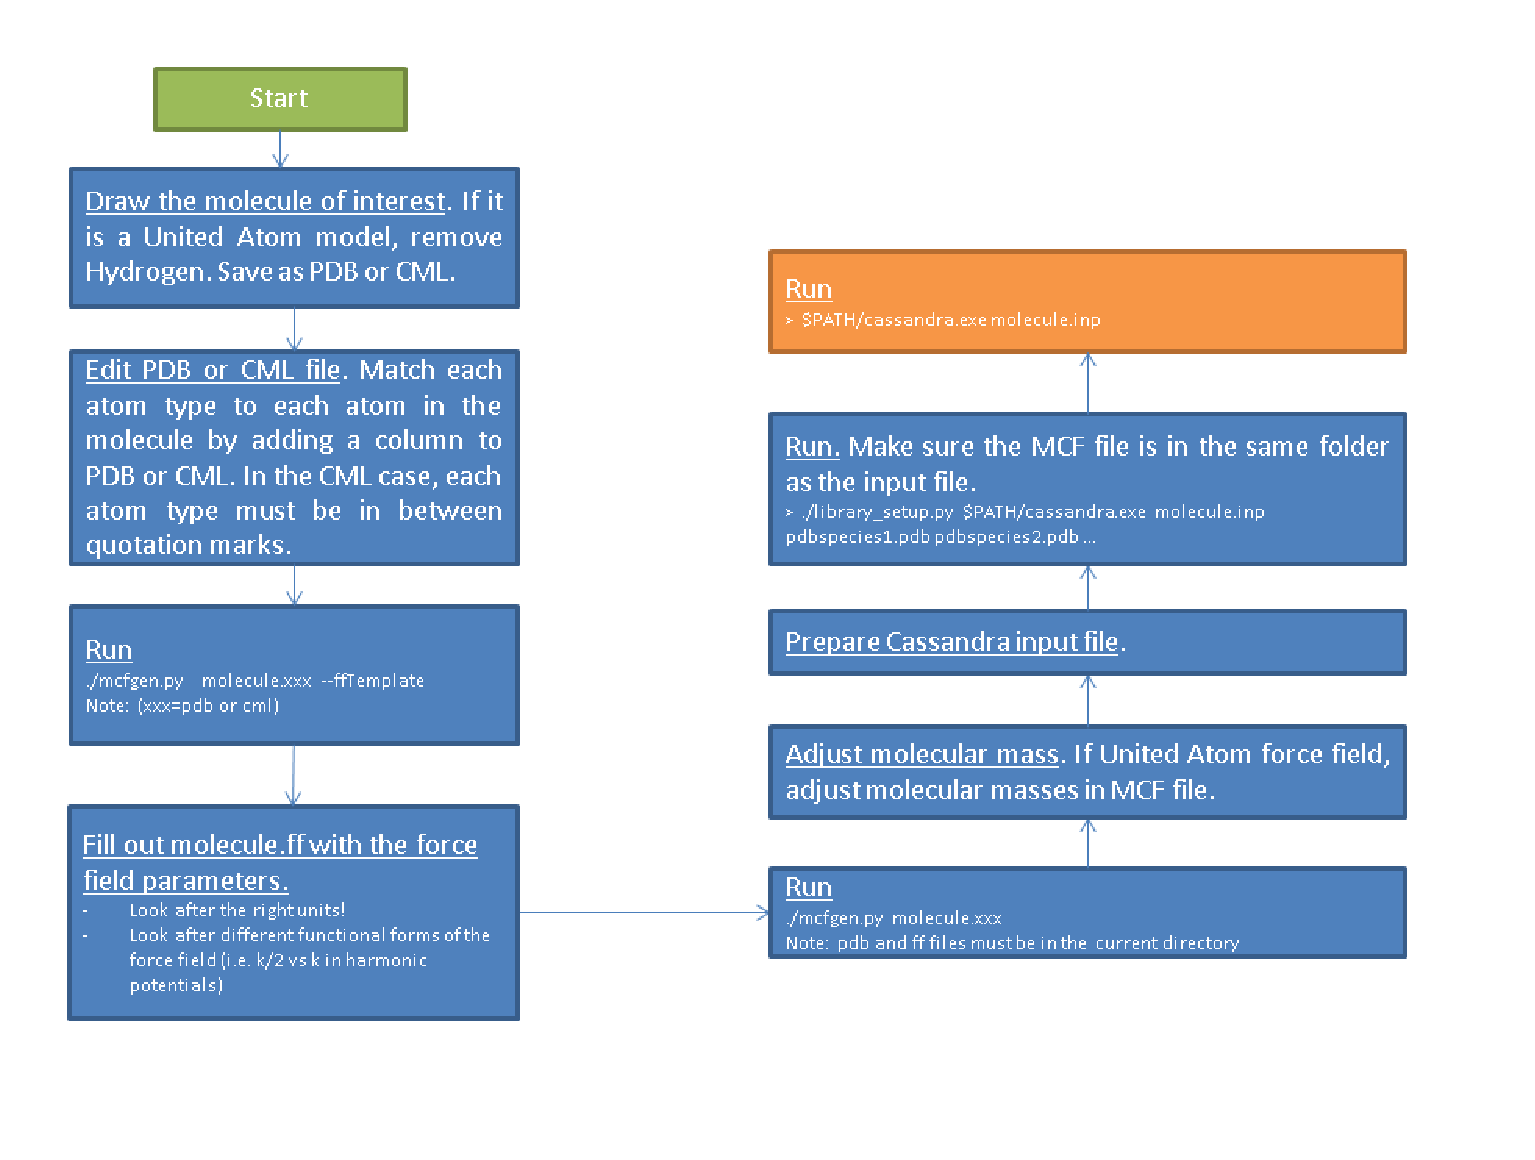
\includegraphics[width=\linewidth]{setup_flowdiagram.eps}
\caption{Flow diagram representing a typical setup of a Cassandra simulation}\label{fig:flow_diagram}
\end{figure}




\section{Cassandra Simulation Setup}

Once a system is identified, setting up a Cassandra simulation from
scratch requires preparation of the following files. \\

\begin{itemize}
\item A molecular connectivity file (MCF)  (*.mcf) containing the molecular
  connectivity information on bonds, angles, dihedrals, impropers and
  whether the molecule is composed of fragments. For information on
  the MCF file, please refer to~\autoref{sec:MCF_File}.

\item An input file (*.inp) (See~\autoref{Sec:Input_File})

\item If the molecule is composed of fragments, then a fragment library file for each of the fragments is required. For instructions on how to generate these files, please refer to the
section \ref{utility:libgen}.

\end{itemize}
%
MCF files for united-atom models of methane, isobutane, dimethylhexane, cyclohexane and diethylether are provided in the \texttt{MCF} directory. Input files for NVT, NPT, GCMC and GEMC ensembles are located in the \texttt{Examples} directory which also contains fragment library files for a number of molecules simulated in these ensembles. 

%Examples of MCF, input files and fragment library files  can be found in the MCF and
%Examples directories repsectively. Fragment files are also located in the
%NVT - diethyether
%NPT - Water\_SPCE, Pentane, diethyether
%GCMC - Methane
%GEMC - Cyclohexane, Methane, Isobutane, Diethyether, Dimethylhexane

\section{Cassandra File Preparation}

\subsection{MCF File}
One MCF file is required for each unique species in a simulation. A
species is defined as a collection of atoms associated with each other
through bonds. Thus a molecule is a species as is an ion. If you
wanted to simulate sodium sulfate, you would need separate MCF files
for the sodium ion and the sulfate ion. MCF files can be created manually 
or by using the scripts provided with the code, as described in
the section \ref{utility:mcfgen}. Instructions for generating an MCF file can also be found in the \texttt{Scripts/MCF\_Generation/README} file. 
We will collect MCF files submitted to us by users and will post them on the Cassandra
website http://cassandra.nd.edu. If you have an MCF file you would
like us to post, send it to ed@nd.edu.
%
%
\subsection{Input File}
%
%
An input file is required for a Cassandra simulation. The input file
specifies conditions for the simulation and various keywords required
for the simulation in a given ensemble. Please refer to 
Chapter~\ref{Sec:Input_File}  for further details.
%
\subsection{Fragment Library Generation}
Cassandra makes use of reservoir sampling schemes to sample correctly and efficiently various coupled intramolecular degrees of freedom associated with
branch points and rings. Details may be found in our
publication~\cite{Shah:2011}. The idea is to decompose the entire
molecule into fragments that are either branch points or ring groups,
each coupled to other fragments via a single dihedral angle. Thus, the
total number of fragments of a molecule is the sum of branch points
and ring groups in the molecule. The neighboring fragments are
connected by two common atoms present in each of the fragments. Note
that the ring group contains all the ring atoms and those directly
bonded to the ring atoms. For each fragment identified, Cassandra runs
a pre\textendash simulation in the gas phase to sample the intramolecular degrees
of freedom. A library of a large number of these conformations are
stored for use in an actual simulation. \\ \\
%
%
The gas phase library generation has been automated with the script \texttt{library\_setup.py} located in the \texttt{Scripts/Frag\_Library\_Setup}
directory. Use the following command for generating the fragment library. \\ \\
%
\texttt{> python path\_to\_Scripts/Frag\_Library\_Setup/library\_setup.py cassandra\_executable \\ input\_filename mol1.pdb (mol1.cml)  mol2.pdb (mol2.cml) ...}\\ \\
%
where \texttt{input\_filename} is the name of the input file for the actual simulation and \texttt{mol1.pdb mol2.pdb ...} or \texttt{mol1.cml mol2.cml ...} correspond to the
names of the pdb (or cml) files used to generated the MCF files. Make sure that if a file does not exist in the current working directory, its path relative
to the current working directory is specified. 

%If the molecule is not represented as a collection of fragments, then
%an initial configuration can be generated by simply supplying the name
%of the input file to the cassandra executable \\ \\
%%
%{\it \$cassandra\_path/cassandra.exe \$input\_file}.\\ \\
%%
%However, if the molecule is composed of fragments, two intermediate
%steps are required before a simulation is started: \\ 
%%
%\begin{itemize}
%\item Generation of mcf, xyz and car files for each fragment,
%\item Using the fragment mcf files to generate fragment conformations
%  at the temperature of the simulation. Thus, the fragment
%  conformations need to be regenerated if the simulation temperature
%  is changed.
%\end{itemize}
%
%\section{Cassandra Analysis}
%At present, Cassandra does not come with any analysis tools except a
%simple plotting script 'analysis.py'. The analysis script takes in the
%name of the input file as an argument. The analysis script will then
%figure out the number of properties specified in the input file and an
%xmgrace plot will be produced for each property as a function of Monte
%Carlo steps. Users should ensure that thermodynamic properties are
%converged for accurate average calculations.

\section{Running a Simulation}

To launch a Cassandra simulation, run the following command: \\ \\
%
\texttt{> cassandra\_executable input\_filename} \\ \\
%
The executable will read \texttt{input\_filename} and execute the instructions. Make sure that the required files (MCF, fragment library files) are located in the directories as given in the input file.

\section{Restarting a Simulation}
Restarting a simulation requires either a checkpoint file (*.chk produced
by Cassandra) or a configuration file obtained from xyz files generated
from a previous simulation. For the set up of these simulations, a script
in \texttt{Scripts/Read\_Old} is provided. Detailed instructions are contained
in the README file in this directory. 

%The 'checkpoint' option in the '\# Start\_Type' can be used to restart
%a simulation from a checkpoint file generated from a previous
%simulation. {\em An error in reading the checkpoint file
%  may occur if the '\# Sim\_Type' is not identical for both the simulations.'}
%
%When this option is used, the checkpoint file will be used
%to initialize the following variables.
%
%\begin{itemize}
%\item Total number of trials for displacement, rotation, dihedral and
%  angle moves for each species in every box.
%\item Total number of successful attempts for displacement, rotation,
%  dihedral and angle moves for each species in every box.
%\item Total number of successful volume moves and total number of
%  volume moves performed for each box in a simulation that involves
%  volume fluctuations.
%\item Total number of trials performed in each box.
%\end{itemize}
%
%The following variables will be {\em overwritten} by the checkpoint
%file. 
%
%\begin{itemize}
%\item Maximum displacement width, maximum rotational width and
%  torsional width for each species in every box.
%\item Box shapes
%\item Box lengths
%\item Maximum volume fluctuation for each box.
%\item Pore width and maximum change in pore width for a slit pore
%  simulation.
%\item Random number seeds.
%\end{itemize}
%
%\section{Restart Simulation - 'read\_old'}
%The 'read\_old' option in the '\# Start\_Type' can be used restart a
%simulation from a file that contains only the information about number
%of molecules of each species in a given box and the coordinates. One
%input file is required for each box. The following procedure may be
%used to generated the last configuration file suitable for input to a
%Cassandra simulation.
%
%\begin{itemize}
%\item From the last output in the '\$input\_file\_Mov\_H.box*, extract
%  the information about the total volume, cell matrix,  number of
%  species and number of moles of each species in the box.
%\item From the last output in the '\$input\_file\_Mov\_XYZ.box*,
%  extract the last configuration.
%\item Open a new file named '\$input\_file.old.box*'.
%\item The first line will contain number of molecules of each species
%  in box*.
%\item Append the last configuration in the box obtained above.
%\end{itemize}
%
%
%
% Fragment generation
%
%
%
%\section{Fragment Generation}
%Cassandra uses an advanced configurational bias Monte Carlo scheme~\cite{Shah:2011,Macedonia:1999} for conformational sampling and insertion\/deletion of molecules. In this scheme, a molecule is decomposed into fragments and a conformational library, satisfying the bond angle probability distribution, for each of the fragments is generated in the gas-phase. The molecule is reconstructed by joining the fragments who conformations are chosen from these gas phase libraries. To carry out fragment-base simulation requires two steps: \\
%\begin{itemize}
%\item Generation of fragments for a given molecule.
%\item Generation of conformational library
%\end{itemize}
%%
%\subsection{Generation of fragments}
%This step is necessary to generate individual fragment MCF and CAR files that can be used for fragment library generation. For this step, a master MCF file of the parent molecule must be prepared. The '\# Sim\_Type' for this simulation is set to 'MCF\_Gen'. Note that, if there are ring atoms in the molecule, they must be explicitly identified in the master MCF file. {\bf At present, the code  identifies only non-ring fragments}. A sample input file is provided. At the successful completion of fragment generation, the user will see a number of files, such as {\em fragment\_1\_1.mcf, fragment\_1\_1.car} and corresponding xyz file and so on. Here the first index refers to the fragment while the second index refers to the species id.  For the generation of the CAR and XYZ files, the anchor atom is placed at the origin while other atoms are placed randomly on a sphere the radius of which is equal to the bondlength. 
%%
%If there are any rigid fragments in the molecule, the CAR and XYZ file coordinates generated at this step are not appropriate for actual simulations. See below.
%%
%\subsection{Generation of Fragment Library}
%%
%Once the MCF and CAR files are generated, an additional step of generating the conformational library for each of the unique fragments is carried out. Two fragments are considered identical if they contain same number of atoms; all the bond lengths are identical; the nominal values of all the bond angles are the same and so are the force constants.  For the library generation, an NVT Monte Carlo simulation is carried out with a single molecule in the gas phase. The '\# Sim\_Type' for such simulations are 'NVT\_MC\_Fragment' or 'NVT\_MC\_Ring\_Fragment' depending on whether a given fragment has cyclic fragments. Sample input files are provided for the user. In the non-ring fragment library generation, atom sampling algorithm is carried out to populate the fragment library. For ring fragment, flip move is performed in addition to the atom sampling for the library generation. Details of the algorithm can be found in Shah and Maginn~\cite{Shah:2011}.

\section{Cassandra Output Files}

Cassandra generates several output files which can be used for later analysis. All have as a prefix the Run\_Name specified in the input file. See Chapter \ref{Sec:Input_File} for details. The type of output is specified by the file name suffix. The following are generated:

\begin{itemize}

\item {\bf Log file} (*.log): Contains basic information on what the run is, timing information and reports the various parameters specified by the user. A complete copy of the input file is reproduced. Other important information includes the move acceptance rates. You can use the log file to keep track of what conditions were simulated.

\item {\bf Coordinate file} (*.box\#.xyz): For each box in the system, a set of xyz coordinates are written out with a frequency specified by the user (Coord\_Freq). The file has as a header the number of atoms in the box. Following this, the atomic coordinates of molecule 1 of species 1 are written, then the coordinates of molecule 2 of species 1 are written, etc. After all the coordinates of the molecules of species 1 are written, the coordinates of the molecules of species 2 are written, etc. You can use this file to do all your structural analysis and post processing.\\

Note that if you generate your initial configuration using the make\_config command, the first ``snapshot'' of the coordinate file
will contain the initial configuration of all the species in the system for a given box. You can use this configuration to check on whether the initial configuration 
is reasonable, or use it as an input to other codes. Note that the initial configuration will be generated using a configurational biased scheme,  
so it may be a better starting configuration that if you used other methods. 

\item {\bf Checkpoint file} (*.chk): A checkpoint file is written every Coord\_Freq steps. This can be used to restart a simulation from this point using all of the same information as the run that was used to generate the checkpoint file. To do this, you must use the checkpoint restart option (see Chapter \ref{Sec:Input_File}). It will basically pick up where the simulation left off, using the same random number seed, maximum displacements, etc. This is useful in case your job crashes and you want to continue running a job. You can also use the checkpoint file to start a new simulation using the  configuration of the checkpoint file as an initial configuration and the optimized maximum displacements.  To do this, use the script read\_old.py. You will need to set a new random number seed if you do this. See the documentation in Chapter \ref{Sec:Input_File} for more details.

\item {\bf H-matrix file} (*.box\#.H): This file is written to every Coord\_Freq MC steps. The first line is the box volume in angstrom$^3$. The next three lines are the box coordinates in angstrom in an H-matrix form. Since Cassandra only supports cubic boxes at the moment, this is just a diagonal and symmetric matrix, but is included here for later versions that will enable non-orthogonal boxes. After this, a blank line is written. The next line is the box number, and the final line(s) is(are) the species ID and number of molecules for that species in this box. If there are three species, there will be three lines. This output is repeated every Coord\_Freq times. This file allows you to compute the density of the box during constant pressure simulations.  


\item{{\bf Property file}} (*.box\#.prp\#): This file lists the instantaneous thermodynamic and state properties for each box. Note that you can have more than one property file (hence the\# after `prp') and more than one box (also why there is a \# after `box'). The user specifies which properties are to be written and in what order, and these are then reproduced in this file. The file is written to every Prop\_Freq steps. A header is written to the first two lines to designate what each property is. You may use this file to compute thermodynamic averages.

\end{itemize}

\chapter{Files Required to Run Cassandra}
\label{ch:input_files}

\section{Simulation Input File} \label{sec:Input_File}
This is a required file that is given as an argument to the Cassandra executable.
Example input files for each ensemble are provided in the Examples directory that can be
modified for new simulations.
%Alternatively, input files can be generated using the graphical user interface as
%explained in section \ref{sec:GUI}.
The input file is divided into sections.
Each section begins with a section header that starts with a '\#',
e.g. {\tt\# Run\_Name}, and ends with a blank line.
Section {\tt\# Move\_Probability\_Info} is an exception and terminates with
{\tt\# Done\_Move\_Probability\_Info}, because subsections
e.g. {\tt\# Prob\_Translation} are separated by blank lines.
Comment lines begin with `!' and are ignored.
Sections in the input file can be listed in any order,
but the order and format of keywords and parameters given in each section
are important unless otherwise noted below.
Previously, some keywords were capitalized, e.g. {\tt CUBIC},
some contained an initial capital, e.g. {\tt Units},
and some were all lowercase, e.g. {\tt kappa\_ins}.
New in version 1.2, all keywords are supported in lowercase text;
each word in a section header must still begin with an initial capital.
%
%%%%%%%%%%%%%%%%
%
% # Run_Name
%
%%%%%%%%%%%%%%%%
\subsection{Run Name}\label{sec:Run_Name}
{\bf \# Run\_Name}\\
{\it Character} \\ \\
%
The run name is specified on the next line following the keyword. This name is used as a prefix for all the files
produced by the simulation. For example,\\ \\
%
{\tt{
\# Run\_Name \\
dee.out
}} \\ \\
%
Cassandra will then use \texttt{dee.out} as prefix for all output files created.

%
%%%%%%%%%%%%%%%%
%
% # Sim_Type
%
%%%%%%%%%%%%%%%%
\subsection{Simulation Type}\label{sec:Sim_Type}

{\bf \# Sim\_Type} \\
{\it Character} \\ \\
%
Sets the ensemble (and thus the suite of moves) of a Cassandra simulation.
The following ensembles are supported: \\
\begin{itemize}
\item nvt or nvt\_mc (canonical ensemble)
\item npt or npt\_mc (isothermal-isobaric ensemble)
\item gcmc (grand canonical ensemble)
\item gemc (Gibbs ensemble)
\item gemc\_npt (Multi-species Gibbs ensemble)
\item nvt\_min (canonical ensemble, only moves which lower the energy are accepted)
\item fragment or nvt\_mc\_fragment (canonical ensemble simulation of a fragment)
\item ring\_fragment or nvt\_mc\_ring\_fragment (canonical ensemble simulation of a ring fragment)
\end{itemize}
Simulation types {\tt fragment} and  {\tt ring\_fragment} are
used only for generating a fragment library.
For example, \\ \\
\texttt{
\# Sim\_Type \\
npt \\ \\
}
%
will run a Monte Carlo simulation in the isothermal-isobaric ensemble in which the number of
molecules of each species $N$, the pressure $P$ and temperature $T$ are held constant.
%
%%%%%%%%%%%%%%%%
%
% # Nbr_Species
%
%%%%%%%%%%%%%%%%
\subsection{Number of species}\label{sec:Nbr_Species}
{\bf \# Nbr\_Species} \\
{\it Integer} \\ \\
%
Total number of species in the simulation. For ionic systems, each ion
is counted as a separate species. For example, for a mixture of two
species, use the following: \\  \\
%
\texttt{
\# Nbr\_Species \\
2
}
%
%%%%%%%%%%%%%%%%
%
% # VDW_Style
%
%%%%%%%%%%%%%%%%
\subsection{VDW Style}\label{sec:VDW_Style}
{\bf \# VDW\_Style} \\
{\it Character(i,1)} [{\it Character(i,2) Real(i,3) Real(i,4)/Logical(i,4)}] \\ \\
%
This keyword specifies the functional form of repulsion dispersion
interactions to be used and if tail corrections are added for box $i$.
One line is required for each box.
{\it Character(i,1)} specifies the van der Waals model and can be
\texttt{lj} for a Lennard-Jones 12-6 potential,
\texttt{mie} for a Mie potential,
or \texttt{none} to turn off all repulsion-dispersion interactions.
{\it Character(i,2)} and {\it Real(i,3)} are required for \texttt{lj} or \texttt{mie}.
{\it Character(i,2)} specifies how the Lennard-Jones potential is truncated.
Options are \texttt{cut}, \texttt{cut\_tail}, \texttt{cut\_switch}, or \texttt{cut\_shift}.
Refer to Chapter~\ref{Chapter:Force Field} for the functional forms.
The other parameters \emph{Real(i,3)} and \emph{Real(i,4)/Logical(i,4)} depend on the
selection of \emph{Character(i,2)} as described below:
%
\begin{itemize}
\item \textbf{cut}: This option cuts the  potential at the distance
specified by \emph{Real(i,3)}. The fourth parameter is omitted. \\ \\
%
For example, to simulate one box with a 14 \AA\ cutoff specify the following:
\\ \\
\texttt{
\# VDW\_Style \\
lj cut 14.0 } \\ \\
%
Similarly, for a two box simulations such as used in the Gibbs
ensemble where both boxes have a 14 \AA\ cutoff, use the
following: \\ \\
\texttt{
\# VDW\_Style \\
lj cut 14.0 \\
lj cut 14.0 } \\ \\
%
\item \textbf{cut\_tail}: This options cuts the potential off at a distance
corresponding to \emph{Real(i,3)} and applies analytic tail
corrections to the energy and pressure. An optional fourth argument
\emph{Logical(i,4)} can be set
to 'true', in which case \emph{Real(i,3)} is ignored and the cutoff
distance is always set to half of the simulation box length. The
cutoff will change during the course of the simulation when attempting
volume moves.  This option is provided to enable reproduction of
literature simulations that use a cut off distance of half the
simulation box length, but its use is discouraged. \\ \\
%
For example, to simulate one box with a 14 \AA\ cutoff using tail
corrections, specify the following:
\\ \\
\texttt{
\# VDW\_Style \\
lj cut\_tail 14.0 } \\ \\
%
For a two box simulation where the first box has a 14 \AA\ cutoff and
the second one has a 20 \AA\ cutoff, use the
following:
\\ \\
\texttt{
\# VDW\_Style \\
lj cut\_tail 14.0 \\
lj cut\_tail 20.0 } \\ \\
%
\item \textbf{cut\_switch}: This option cuts the potential off and smoothly
brings the potential to zero using a spline. The potential is cutoff
and the spline turned on at a distance specified by \emph{Real(i,3)}
(r$_{on}$ in Eq~\ref{Eq:cut_switch}) and the potential goes
to zero at a distance specified by \emph{Real(i,4)} (r$_{off}$ in
Eq~\ref{Eq:cut_switch}). \\ \\
%
For example, a one box simulation using the cut\_switch option could be
specified as follows:
\\ \\
\texttt{
\# VDW\_Style \\
lj cut\_switch 12.0 14.0} \\ \\
%
In this case, the Lennard-Jones potential would end at 12.0 \AA\ and
be smoothly taken to zero at 14.0 \AA. $r_{on} < r_{off}$ or \emph{Real(i,3)} $<$ \emph{Real(i,4)}.
%
\\ \\
\item \textbf{cut\_shift}: This option cuts the potential off at a distance
specified by \emph{Real(i,3)} and shifts the entire potential so that
at this distance the potential is zero. The fourth parameter
\emph{Real(i,4)/Logical(i,4)} is omitted. The functional form of this
potential is given in eq~\ref{Eq:cut_shift}. \\ \\
%
To perform a two box simulation with a cut\_shift option in which both
boxes have a 10.5 \AA\ cutoff, use the following:
\\ \\
\texttt{
\# VDW\_Style \\
lj cut\_shift 10.5 \\
lj cut\_shift 10.5 } \\ \\
%
\end{itemize}
{\bf Note: For all options, cutoff distances must be less than or
  equal to the shortest edge length of a simulation box}.
%%%%%%%%%%%%%%%%
%
% # Charge_Style
%
%%%%%%%%%%%%%%%%
\subsection{Charge Style}\label{sec:Charge_Style}
{\bf \# Charge\_Style} \\
{\it Character(i,1)} [{\it Character(i,2) Real(i,3) Real(i,4)}] \\ \\
%
Cassandra allows the use of fixed partial charges on atomic centers
using a Coulomb potential of the form given in Eq~\ref{Eq:Coulomb}.
If this section is missing from the input file,
the electrostatic energy of the simulation will not be computed.
If you do not wish to use a Coulomb potential for box {\em i},
set {\it Character(i,1)} to \texttt{none}. If \texttt{none} is
selected for {\it Character(i,1)} then {\it Character(i,2)},
{\it  Real(i,3)} and {\it Real(i,4)} are omitted.
\\ \\
For example, \\ \\
\texttt{
\# Charge\_Style \\
none}
\\ \\
should be used if you have no partial charges and are simulating a single box
(or the section can just be omitted).

To compute the electrostatic energy for box {\em i},
this section must be included and {\it Character(i,1)} set to \texttt{coul}.
For this option,
{\it Character(i,2)} can be set to \texttt{ewald} if you want to use
an Ewald sum to compute Coulombic interactions, \texttt{dsf} if you want to use
the Damped Shifted Force method by Fennell \textit{et al.}\cite{Fennell:2006}, or it can be set to
\texttt{cut}, in which case the Coulombic interactions will be cut off and
the long range interactions ignored. For the Ewald option,
{\it Real(i,3)} is the real space cutoff distance and {\it Real(i,4)}
specifies the accuracy of the Ewald summation. A reasonable value for
the accuracy is 10$^{-5}$. Note that the number of reciprocal vectors
for the Ewald summation is determined in the code based on the
accuracy parameter. For more details, see the paper by Fincham
\cite{Fincham:1994}.\\ \\
%
For example,
\\ \\
\texttt{
\# Charge\_Style \\
coul ewald 12.0 1E-5}\\ \\
will use the Ewald sum for a single box. The real space cutoff will be
12 \AA\ and the accuracy will be $10^{-5}$. If you have two boxes,
like in a Gibbs ensemble calculation, then you could use the
following:
\\ \\
\texttt{
\# Charge\_Style \\
coul ewald 12.0 1E-5\\
coul ewald 30.0 1E-5}
\\ \\
This will use an Ewald sum for both boxes. In the first box, the real
space cutoff will be 12 \AA\ while in the second box a larger cutoff
of 30 \AA\ will be used. {\bf Note: When performing Gibbs ensemble
simulations of vapor-liquid equilibria, the vapor box is often much
larger than the liquid box. In this case, you will want to use a
longer real space cutoff for the larger vapor box to avoid using too
many reciprocal space vectors.} Also note that the real space
cutoffs must always be less than or equal to half of the shortest edge
length of a simulation box. \\

If you wish to use the Damped Shifted Force method, the entry {\it Real(i,3)}
is the electrostatic energy cutoff distance and {\it Real(i,4)} is an optional
entry to specify the damping parameter. If not specified, Cassandra will
set this value algorithmically from the cutoff radius. For example,
\\ \\
\texttt{
\# Charge\_Style \\
coul dsf 12.0 0.20}\\

will use the Damped Shifted Force method for a single box. The electrostatic
energy cutoff will be set to 12 \AA\ and the damping parameter will be set
to 0.20, which is a reasonable value for
typical liquid phase simulations. \\  \\
%
{\bf{Note}}: If the cutoff in VDW\_Style is set to half of the
simulation box length, any cutoff distance specified in the
Charge\_Style section will default to the half of the simulation box
length. In the case of Ewald summation, however, the accuracy will be
the same as {\it Real(i,4)}.
%
%%%%%%%%%%%%%%%%
%
% # Mixing_Rule
%
%%%%%%%%%%%%%%%%
\subsection{Mixing Rule}\label{Mixing_Rule}
{\bf \# Mixing\_Rule} \\
{\it Character} \\ \\
%
Sets the method by which van der Waals interactions between unlike atoms are calculated.
Acceptable options are \texttt{lb} for Lorentz-Berthelot,
\texttt{geometric} for geometric mixing rule
and \texttt{custom} for allowing the user to provide specific values.
To use either \texttt{lb} or \texttt{geometric} keywords with the Mie potential,
all atomtypes must have the same repulsive and dispersive exponents.
If this section is missing, \texttt{lb} is used as default. \\

To illustrate the use of the \texttt{custom} option, consider a mixture of methane (species 1)
and butane (species 2) united atom models using a Lennard-Jones potential.
Methane has a single atomtype, CH4.
Butane has two atomtypes: pseudoatoms 1 and 4 are type CH3, pseudoatoms 2 and 3 are type CH2.
The cross interaction table is as follows:

\texttt{
{\bf \# Mixing\_Rule} \\
custom\\
CH4  CH3  120.49   3.75\\
CH4  CH2   82.51   3.83\\
CH3  CH2   67.14   3.85\\
}
\\ \\
The order in which atom types are listed is unimportant,
but the atom types must match exactly the types given in each MCF.
The Lennard-Jones potential requires two parameters:
an energy parameter with units K, and a collision diameter with units \AA.
The Mie potential requires four parameters:
an energy parameter with units K, a collision diameter with units \AA,
a repulsive exponent, and a dispersive exponent.

%%%%%%%%%%%%%%%%
%
% # Seed_Info
%
%%%%%%%%%%%%%%%%
\subsection{Starting Seed}\label{sec:Seed_Info}
{\bf \# Seed\_Info} \\
{\it Integer(1) Integer(2)} \\ \\
%
Inputs for the starting random number seeds for the simulation.
Cassandra uses a random  number generator proposed by L'Ecuyer \cite{random_gen:1999},
which takes five seeds to calculate a random number,
out of which three are defined internally while two {\it Integer(1)} and
{\it Integer(2)} are supplied by the user.
{\bf When a `checkpoint' file is used to restart a
simulation (see \# Start\_Type below), the user supplied seeds will be
overwritten by those present in the checkpoint file.
If \# Start\_Type is set to `read\_config',
then the seeds specified in the input file are used}.  \\ \\
As an example, \\ \\
\texttt{
\# Seed\_Info \\
1244432 8263662
} \\ \\
is an acceptable way of specifying the seeds.
Note that two independent simulations can be run using the same input
information if different seeds are used.
If two simulations having exactly the same input
information and the same seeds are run, the results will be identical.
%
%%%%%%%%%%%%%%%%
%
% # Rcutoff_Low
%
%%%%%%%%%%%%%%%%
\subsection{Minimum Cutoff}\label{sec:Rcutoff_Low}
{\bf \# Rcutoff\_Low} \\
{\it Real} \\ \\
%
Sets the minimum allowable distance in \AA\ between two atoms.
Any MC move bringing two sites closer than this distance will be immediately rejected.
It avoids numerical
problems associated with random moves that happen to place atoms very
close to one another such that they will have unphysically strong repulsion or
attraction. This distance must be less than the intramolecular
distance of all atoms in a species which are not bonded to one
another. For models that use dummy sites without explicitly defining
bonds between dummy and atomic sites of the molecules (for example,
the TIP4P water model), it is important that the minimum distance is set to be less
than the shortest distance between any two sites on the molecule. For
most systems, 1 \AA\ seems to work OK, but for models with dummy
sites, a shorter value may be required.
%%%%%%%%%%%%%%%%
%
% Pair_Energy
%
%%%%%%%%%%%%%%%%
\subsection{Pair Energy Storage}\label{sec:Pair_Energy}
{\bf \# Pair\_Energy} \\
{\it Logical} \\ \\
%
Cassandra can use a time saving feature in which the energies between
molecules are stored and used during energy evaluations after a move,
thereby saving a loop over all molecules.
This requires more memory, but it can be faster.
The default is to not use this feature.
If you wish to use this, set {\it Logical} to `true'.
%%%%%%%%%%%%%%%%%%%%%%%%%%%%%%%%%%%%%%%%%%%%%%%%%%%%%%%%%%
%
% State point related information
%
%%%%%%%%%%%%%%%%%%%%%%%%%%%%%%%%%%%%%%%%%%%%%%%%%%%%%%%%%%
%%%%%%%%%%%%%%%%
%
% Molecule_Files
%
%%%%%%%%%%%%%%%%
\subsection{Molecule Files}\label{sec:Molecule_Files}
{\bf \# Molecule\_Files} \\
{\it Character(i,1) Integer(i,2)}  \\ \\
%
This specifies the name of the molecular connectivity file (MCF) and
the maximum total number of molecules of a given species specified by this MCF.
A separate line is required for each species present in the simulation.
{\it Character(i,1)} is the name of the MCF for species {\it i}.
{\it Integer(i,2)} is the maximum number of molecules expected for the species.  \\ \\
%{\it Integer(i,3)} is
%optional argument that is required in a CFC simulation and indicates
%number of fractional particles of the species in the simulation. For
%example, in a Gibbs ensemble simulation for phase equilibria, there
%will be two fractional particles. \\ \\
For example \\ \\
\texttt{
\# Molecule\_Files \\
butane.mcf 100 \\
hexane.mcf 20\\
octane.mcf 5} \\ \\
specifies that there are three different species, and the MCFs
state the names of the files where information on the three species
can be found.
Species 1 is butane, species 2 is hexane and species 3 is octane.
There can be a maximum of 100 butane molecules, 20 hexane molecules
and 5 octane molecules in the total system.
The maximum
number of molecules specified here will be used to allocate memory for
each species, so do not use larger numbers than are needed.
%%%%%%%%%%%%%%%%
%
% # Box Info
%
%%%%%%%%%%%%%%%%
\subsection{Simulation Box}\label{sec:Box_Info}
{\bf \# Box\_Info} \\
{\it Integer(1)} \\
{\it Character(i)}  \\
{\it Real(i,1)} [{\it Real(i,2) Real(i,3)}] \\
{[}{\tt restricted\_insertion} {\it Character(1) Real(1) [Real(2)]}] \\ \\
This section sets parameters for the simulation boxes.
{\it Integer(1)} specifies the total number of boxes in the simulation.
Gibbs ensemble simulations must have two boxes.
{\it Character(i)} is the shape of the $i$th simulation box.
The supported keywords are \texttt{cubic}, \texttt{orthogonal}, and \texttt{cell\_matrix}. \\ \\
%
If {\it Character(i)} is \texttt{cubic}, \emph{Real(i,1)} is the length of the box edges in \AA.
Information for additional boxes is provided in an analogous fashion
and is separated from the previous box by a blank line.
For a two box simulation, box information is given as: \\ \\
%
\texttt{
\# Box\_Info \\
 2 \\
 cubic \\
 30.0  \\
 \\
 cubic \\
 60.0} \\ \\
%
This will construct a 30 x 30 x 30 \AA\ cube and the second a 60 x 60 x 60 \AA\ cube.

The options orthogonal and cell\_matrix are only supported for constant volume simulations
(i.e. NVT or GCMC) which only have 1 box.
If {\it Character(1)} is \texttt{orthogonal}, \emph{Real(1,1) Real(1,2) Real(1,3)} are the length,
width and height that define the simulation box. For example, \\ \\
%
\texttt{
\# Box\_Info \\
 1 \\
 orthogonal \\
 30.0 35.0 40.0} \\ \\
%
This will create a simulation box with dimensions 30.0 x 35.0 x 40.0 \AA. \\ \\
%
A non-orthogonal box is created by setting {\it Character(1)} to \texttt{cell\_matrix}.
In this case, three basis vectors are needed to define the simulation box.
Each vector is entered as a column of a 3x3 matrix.
For example, \\ \\
%
\texttt{
\# Box\_Info \\
 1 \\
 cell\_matrix \\
 30 ~0 ~0\\
\hspace*{0.5em}0 35 ~0\\
\hspace*{0.5em}0 ~2 40} \\ \\
%
defines a simulation box with basis vectors (30, 0, 0), (0, 35, 2) and (0, 0, 40).

The optional keyword \texttt{restricted\_insertion} is used to define a region inside the simulation box
in which molecules will be inserted at start-up via \texttt{make\_config} or \texttt{add\_to\_config}
or throughout the simulation via grand canonical insertion moves or Gibbs ensemble swap moves.
\texttt{restricted\_insertion} takes one of several options:
\texttt{sphere}, \texttt{cylinder}, \texttt{slitpore}, \texttt{interface}.
Each option requires additional parameters, as follows.

\begin{itemize}
	\item \texttt{sphere} $R$,
	where $R$ is the radius of a sphere centered at the origin
	\item \texttt{cylinder} $R$,
	where $R$ is the radius of a cylinder centered on the z-axis
	\item \texttt{slitpore} $z_{max}$,
	where $z_{max}$ is half the height of a rectangular prism centered on the {\it xy}-plane
	\item \texttt{interface} $z_{min}$ $z_{max}$,
	defines two rectangular prisms that span the box in the {\it x} and {\it y} directions.
	One box has bounds $z_{min} < z < z_{max}$ and the other has bounds $-z_{max} < z < -z_{min}$.
\end{itemize}

For example, to make a spherical droplet with a radius of 5 \AA\ in cubic box 100 \AA\

\texttt{
\# Box\_Info \\
	1 \\
	cubic \\
	100 \\
	restricted\_insertion sphere 5.0} \\

In addition, the insertion method for each species must be identified in the
\texttt{Start\_Type} or \texttt{Move\_Probability\_Info} sections.

%
%If it's \texttt{SLIT\_PORE} geometry then it is assumed
%that the periodicity is in the xy plane while the slit pore width is
%along the z  In this case {\it
%  Real(i,3) Real(i,4)} provide box dimensions in the x and y
%directions respectively. {\it Real(i,5)} is the pore width if there
%Ewald summation is not enabled. If the simulation uses Ewald summation
%then {\it Real(i,5)} will be the length in the z direction for the
%computation of electrostatic energy using 3D Ewald summation. A good
%starting point is twice the pore width. {\bf Users are encouraged to check
%the convergence of the electrostatic energy by varying {\it
%  Real(i,5)}}. The actual pore width will be determined by {\bf \#
%Pore\_Width} keyword (\autoref{sec:Pore_Width}). \\ \\
%
%
%%%%%%%%%%%%%%%%
%
% Temperature_Info
%
%%%%%%%%%%%%%%%%
\subsection{Temperature}\label{sec:Temperature_Info}
{\bf \# Temperature\_Info} \\
{\it Real(i)} \\ \\
%
{\it Real(i)} is the temperature in Kelvin for box $i$.
For GEMC, the temperature of box 2 will be read from a second line: \\ \\
%
\texttt{
\# Temperature\_Info \\
 300.0 \\
 300.0} \\ \\
%
%%%%%%%%%%%%%%%%
%
% Pressure_Info
%
%%%%%%%%%%%%%%%%
\subsection{Pressure}\label{sec:Pressure_Info}
{\bf \# Pressure\_Info} \\
{\it Real(i)} \\ \\
%
{\it Real(i)} is the pressure setpoint in bar for box $i$.
For GEMC, the pressure of box 2 will be read from a second line: \\ \\
%
\texttt{
\# Pressure\_Info \\
 1.0 \\
 1.0} \\ \\
%
If the simulation type does not require an input pressure (e.g., NVT), this section will be ignored.
%%%%%%%%%%%%%%%%%%
%
%  Chemical_Potential_Info
%
%%%%%%%%%%%%%%%%%%
\subsection{Chemical Potential}\label{sec:Chemical_Potential}
{\bf \# Chemical\_Potential\_Info} \\
{\it Real(1) ... Real(n)} \\ \\
%
where {\it n} is the number of insertable species and {\it Real(i)} is the
chemical potential setpoint (shifted by a species-specific constant) of
insertable species {\it i} in kJ/mol. Each chemical potential will be assigned
in the order species appear in the \texttt{Molecule\_Files} section.
For species with insertion method {\tt none},
the chemical potential can be listed as {\tt none} or omitted.
This section is only read for grand canonical simulations.
See Eq. (\ref{eq:muShift}) for more information.
For example, the adsorption of methane (species 2) in a zeolite (species 1)
can be computed by inserting methane molecules into a box with a zeolite crystal.
In this example, only one chemical potential (for methane) is required
and the following are equivalent: \\ \\
%
\texttt{
\# Chemical\_Potential\_Info \\
 -35.0} \\ \\
%
\texttt{
\# Chemical\_Potential\_Info \\
 none -35.0} \\ \\
%
%%%%%%%%%%%%%%%%
%
% Neighbor_Style
%
%%%%%%%%%%%%%%%%
%\subsection{Neighbor Style}\label{Neighbor_Style}
%{\bf \# Neighbor\_Style} \\
%{\it Character(1) Real(2) or Integer(2)} \\ \\
%
%Sets the option for neighbor list in a simulation. {\it Character(1) } sets the type of Neighbor style
%to be used in the simulation. Acceptable choices are \texttt{verlet} or \texttt{linked\_cell}. If \texttt{verlet} then
%only {\it Real(2)} specifying the thickness of the skin is required. If \texttt{verlet} and $r_{cut} + r_{skin}$ is
%greater than the half box length then an error is generated. \\ \\
%
%For \texttt{linked\_cell}, only {\it Integer(2)} is required. This sets the simulation box for which a linked-cell
%list will be generated. At present, generation of only one linked-cell is supported. With this option, if $3*r_{cut}$
%then an error will be produced. \\ \\
%
%In this absence of this keyword, no neighbor list will be used. \\ \\
%%%%%%%%%%%%%%%%
%
% Reaction_Info
%
%%%%%%%%%%%%%%%%
%\subsection{Reaction}\label{sec:Reaction_Info}
%{\bf \# Reaction\_Info} \\
%{\it Integer(1)}\\
%{\bf reaction method} \\
%{\it Character(2)}\\
%{\it Integer(i,j) } Optional \\
%{\bf stoichiometry} \\
%{\it Integer(i) } \\
%{\bf P0 K0 reaction box} \\
%{\it Real(3) Real(4) Integer(5)} \\
%%
%This section provides information if reactions need to be \texttt{carried out} in
%the simulation. {\it Integer(1)} denotes the total number of reactions. The
%{\bf reaction method} is specified as {\it Character(2)} as either a \texttt{CFC}
%or an \texttt{INTEGER} reaction. If \texttt{INTEGER} is specified as the reaction method, then
%the line ``{\it replacement matrix}'' is required followed by the matrix ``{\it Integer(i,j)}''
%are required. This matrix provides information whether products are to be inserted
%in the whole created by the reactants. For example, in the reaction {\it A + B $\rightarrow$ C},
%if C is placed in the hole created by A and vice versa, the matrix would be: \\ \\
%%
%0 0 1 \\
%0 0 0 \\
%1 0 0 \\ \\
%%
%{\it Integer(i)} sets the stochiometric number of each species in a given reaction.
%For the above example, the \texttt{stochiometry} section would look like: \\ \\
%%
%-1 \\
%-1 \\
%1 \\ \\
%%
%{\it Real(3)} is the total pressure of the system while {\it Real(4)} sets the equilibrium
%constant k$^0$ of the reaction and {\it Integer(5)} is the simulation box in which the
%reaction will take place. \\ \\
%%
%The above section is repeated for all the reactions in the system. \\ \\
%%
%%%%%%%%%%%%%%%%%
%%
%% Bin_Info
%%
%%%%%%%%%%%%%%%%%
%\subsection{Bins}\label{sec:Bin_Info}
%{\bf \# Bin\_Info} \\
%{\it Integer(i)} \\
%{\it Real(i,j)} \\
%{\it Integer(1) Integer(2)} \\ \\
%%
%This section is necessary while performing a CFC MC move.
%For each \texttt{sorbate' species, {\it Integer(i)} defines total number of bins and
%{\it Real(i,j)} is the weight of each bin. There must be {\it Integer(i)} entries on
%this line. The weights, for a given sorbate, are specified on separate lines for each box. Note that, in the beginning of a simulation, all the weights may be set to zero and a Wang-Landau scheme may be utilized to refine the
%weights as the simulation proceeds. The Wang-Landau implementation is controlled by two parameters: {\em Integer(1) Integer(2)}. {\em Integer(1)} specifies the number of Wang-Landau updates to be carried out in the simulation
%before setting the weights to a constant. On the other hand, {\em Integer(2)} specifies the number of MC steps to be carried out in a given Wang-Landau cycle.
%%
%
%%%%%%%%%%%%%%%%
%
% Move_Probabilities
%
%%%%%%%%%%%%%%%%
\subsection{Move Probabilities}\label{sec:Move_Probabilities}
{\bf\# Move\_Probability\_Info \\
{[}subsections] \\
\# Done\_Probability\_Info} \\

This section specifies the probabilities associated with different types of
MC moves to be performed during the simulation.
The section begins with the header {\tt \# Move\_Probability\_Info}
and is terminated by the footer {\tt \# Done\_Probability\_Info}.
All the move probability subsections must be between the section header and footer.

If the move probabilities do not sum to 1.0,
then the probability of each move will be divided by the total.
%
%%%%%%%%%%%%%%%%
%
% Cluster move
%
%%%%%%%%%%%%%%%%
%\subsubsection{Cluster}
%{\bf \# Prob\_Cluster\_Move}\\
%{\it Real(1) }\\
%{\it Real(2) } \\
%{\it Real(i,3)} \\
%{\it Real(i,4)} \\
%{\it Logical(j,5)} \\ \\
%%
%Probability of performing a cluster move is denoted by {\it Real(1)}. The radius of
%the cluster is specified by {\it Real(2)}. On the next line, the maximum displacement
%of cluster in each box is given by {\it Real(i,3)}. The probability of perfoming a
%cluster move in each of the boxes is specified by {\it
%  Real(i,4)}. Whether a species $j$ has a special center-of-mass is
%specified by {\it Logical(j,5)}\\ \\
%
%%%%%%%%%%%%%%%%
%
% Translation
%
%%%%%%%%%%%%%%%%
\subsubsection{Translation}
{\bf \# Prob\_Translation}\\
{\it Real(1)} \\
{\it Real(i,1) ... Real(i,n) } *One line required for each box $i$ \\ \\
%
where $n$ is the number of species.
{\it Real(1)} is the probability of performing a center of mass translation move.
{\it Real(i,j)} is the maximum displacement in \AA\ of species $j$ in box $i$.
This subsection is optional in all ensembles. \\ \\
%
For example, if you have three species and two boxes, you could specify
the translation probability as \\ \\
\texttt{
{ \# Prob\_Translation} \\
 0.25 \\
2.0 2.5 1.0\\
12.0 12.0 12.0}
\\ \\
This will tell Cassandra to attempt center of mass translations 25\%
of the total moves. For box 1, the maximum displacement will be 2.0 \AA\ for
species 1, 2.5 \AA\ for species 2, and 1.0 \AA\ for species 3.
For box 2, the maximum displacement for all species is 12.0 \AA . \\ \\
%
For a simulation that involves solid frameworks,
set the maximum displacement of the solid species to zero.
Every molecule in the simulation with a maximum displacement greater than zero
has an equal chance of being moved.
%
%When fragment
%simulation is carried out, the specification of the move is given by \\ \\
%
%{\bf \# Prob\_Translation}\\
%{\it Real(1)} \\
%{\it Real(2) Real(3)} \\ \\
%
%As before, {\it Real(1)} is the probability of translation move while {\it Real(2)}
%and {\it Real(3)} specify the maximum displacement in cosine of the polar angle
%and maximum change in the azimuthal angle, respectively.
%
%%%%%%%%%%%%%%%%
%
% Pair Translation
%
%%%%%%%%%%%%%%%%
%
%\subsubsection{Pair Translation}
%{\bf \# Prob\_Pair\_Translate}
%{\it Real(1)} \\
%{\it Real(i,2)} \\
%{\it Integer(3)} \\
%{\it Real(j,4)} \\
%{\it Integer(j,1) Integer(j,2) } \\ \\
%%
%This section specifies the probability {\it Real(1)} of performing a
%coupled move involving two molecules(ions) of the same or different
%species. {\it Real(i,2)} indicates the cumulative probability of
%performing such a move in the box $i$. The next line contains {\it
%  Integer(3)} specifying number of pairs to be moved in such a
%move. The cumulative probability for the $j^{th}$ pair is given by
%{\it Real(j,4)} and {\it Integer(j,1) Integer(j,2)} indicate the
%indices of the species involved in the pair  $j$. The last two lines
%are repeated for as many pairs as given by {\it Integer(3)}.


%%%%%%%%%%%%%%%%
%
% Rotation
%
%%%%%%%%%%%%%%%%
\subsubsection{Rotation}
{\bf \# Prob\_Rotation}\\
{\it Real(1)} \\
{\it Real(i,1) ... Real(i,n)} *One line required for each box $i$ \\ \\
%
where $n$ is the number of species.
The probability of performing a rotation move is specified by
{\it Real(1)} while {\it Real(i,j)} denotes the maximum rotation
for species $j$ in box $i$ in degrees about the x, y or z-axis.
The axis will be chosen with uniform probability.
This subsection is optional for all ensembles. \\ \\
%
For example, if you are simulating a single species in two boxes,
you could specify the rotational probability as \\ \\
\texttt{
{ \# Prob\_Rotation} \\
 0.25 \\
30.0\\
180.0} \\ \\
%
Twenty-five percent of the attempted moves will be rotations.
Molecules in box 1 will be rotated a maximum of 30\degree\ around the x, y, or z-axis.
Molecules in box 2 will be rotated a maximum of 180\degree\ around the x, y, or z-axis. \\ \\
%
If all species are point particles (such as single-site Lennard-Jones particles),
this section should be omitted.
For a multi-species system,
set {\it Real(i,j)} to zero for point particles and solid frameworks. \\ \\
%
Linear molecules are a special case.
A molecule is identified as linear if all angles in the MCF are fixed at 180\degree .
If a linear molecule were aligned with the axis of rotation,
then the molecular orientation would not be changed.
Therefore, linear molecules are rotated by choosing a random unit vector with uniform probability
without regard to the molecule's current orientation or the maximum rotation.
As with non-linear molecules, if {\it Real(i,j)} is zero, no molecules of species $j$ will be rotated. \\ \\
%
For a single box simulation of a non-linear molecule (species 1), a linear molecule (species 2),
and a point particle (species 3), you could specify \\ \\
%
\texttt{
{\# Prob\_Rotation} \\
 0.25 \\
30.0 10.0 0.0} \\ \\
%
Molecules of species 1 will be rotated a maximum of 30\degree\ around the x, y or z-axis,
molecules of species 2 will be rotated by choosing a random unit vector, and
the point particles will not be rotated.
%
%%%%%%%%%%%%%%%%
%
% Angle perturbation
%
%%%%%%%%%%%%%%%%
\subsubsection{Angle}
{\bf \# Prob\_Angle} \\
{\it Real(1)} \\
A molecule will be selected at random and its angle will be perturbed based on its Boltzmann weighted distribution.
The probability of attempting this move is the only required input. It is specified by {\it Real(1)}. Note that this move is rarely needed since the fragment libraries should already provide efficient sampling of angles. This move, however, may improve sampling of angles for large molecules in the case where parts of its fragments are rarely regrown by a regrowth move.

%
\texttt{
\# Prob\_Angle \\
0.3 \\
} \\
%
This will tell Cassandra to attempt angle moves 30\% of the total moves for all molecules containing angles within a given box.

%%%%%%%%%%%%%%%%
%%%%%%%%%%%%%%%%
%
% Dihedral move
%
%%%%%%%%%%%%%%%%
\subsubsection{Dihedral}
{\bf \# Prob\_Dihedral} \\
{\it Real(1)} \\
{\it Real(1) ... Real(n)} \\

The probability of performing a dihedral move is specified by {\it Real(1)} while
{\it Real(n)} denotes the maximum width of a dihedral angle displacement for each species. The maximum width is given in degrees. Note that this move is rarely needed since the regrowth moves should already provide efficient sampling of dihedrals. This move, however, may improve sampling of dihedrals for large molecules in the case where the parts of its fragments are rarely regrown (albeit a small maximum width is provided).\\ \\
%
\texttt{
\# Prob\_Dihedral \\
0.3 \\
20 0.0 \\
}\\
%
This will tell Cassandra to attempt dihedral moves 30\% of the total moves for all molecules containing dihedrals within a given box.
The maximum dihedral width will be 20\degree\ for species 1 and 0.0\degree\
for species 2. Since the maximum dihedral
width of species 2 is set to 0.0\degree\ in both boxes, no dihedral moves will be
attempted on species 2. Note that a single max dihedral width is provided, even if species 1 may contain many dihedrals. This is also true
for simulations with more than one box. Also note that the same max dihedral width is used for systems containing  more than one box.

%
%%%%%%%%%%%%%%%%
%
% Regrowth
%
%%%%%%%%%%%%%%%
\subsubsection{Regrowth}
{\bf \# Prob\_Regrowth} \\
{\it Real(1)} \\
{\it Real(2,1) ... Real(2,n)} \\ \\
%
where $n$ is the number of species.
A regrowth move consists of deleting part of the molecule randomly and
then regrowing the deleted part via configurational bias algorithm.
This can result in relatively substantial conformational changes for
the molecule, but the cost of this move is higher than that of a
simple translation or rotation. The probability of attempting a
regrowth move is specified by {\it Real(1)} while {\it Real(2,i)}
specifies the relative probability of performing this move on species $i$.
The relative probabilities must sum to 1 otherwise Cassandra will quit with an error.
This subsection is optional for all ensembles. \\ \\
%
For example, if simulating 70 molecules of species 1 and 30 molecules of species 2,
you could specify the following: \\ \\
%
\texttt{
\# Prob\_Regrowth \\
0.3 \\
0.7 0.3 } \\ \\
%
Thirty percent of the attempted moves will be regrowth moves.
Seventy percent of the regrowth moves will be attempted on a molecule of species 1
and the balance of regrowth moves on a molecule of species 2. \\ \\
%
{\it Real(2,i)} should be set to zero for monatomic, linear, or rigid species, including solid frameworks.
%
%%%%%%%%%%%%%%%%
%
% Volume displacement
%
%%%%%%%%%%%%%%%%
\subsubsection{Volume}
{\bf \# Prob\_Volume} \\
{\it Real(1)} \\
{\it Real(2)} \\
{[}{\it Real(3)}] \\ \\
%{\it Integer(1)} *Optional \\ \\
%
{\it Real(1)} is the relative probability of attempting a box volume change.
Since volume changes are computationally expensive, this probability should
normally not exceed 0.05 and values from 0.01-0.03 are typical.
{\it Real(2)} is the maximum volume displacement in \AA$^3$ for box 1.
{\it Real(3)} is the maximum volume displacement in \AA$^3$ for box 2,
and is only required for GEMC-NPT simulations.
The attempted change in box volume is selected from a uniform distribution.
This subsection is required for NPT, GEMC-NPT and GEMC-NVT simulations.
%
For example, if you are simulating a liquid with a single box in the NPT ensemble,
you would specify the following: \\ \\
%
\texttt{
\# Prob\_Volume \\
0.02 \\
300} \\ \\
%
This will tell Cassandra to attempt volume moves 2\% of the
total moves. The box volume would be changed by random amounts ranging from
-300 \AA$^3$ to +300 \AA$^3$. For a liquid box 20 \AA\ per side,
this would result in a maximum box edge length change of about 0.25
\AA, which is a reasonable value.
Larger volume changes should be used for vapor boxes.
%
If you wish to perform a GEMC-NPT simulation, you might specify the
following: \\ \\
%
\texttt{
\# Prob\_Volume \\
0.02 \\
300 \\
5000} \\ \\
%
This will tell Cassandra to attempt volume moves 2\% of the
total moves. The first box volume (assumed here to be smaller and of higher
density, such as would occur if it were the liquid box) would be
changed by random amounts ranging from
-300 \AA $^3$ to +300 \AA $^3$. The second box volume would be
changed by random amounts ranging from
-5000 \AA $^3$ to +5000 \AA $^3$. As with all move probabilities, you
can experiment with making
larger or smaller moves. Note that if the \# Run\_Type is set
to {\tt equilibration}, Cassandra will attempt to optimize the magnitude of
the volume change to achieve about 50\% acceptance rates.

The volume perturbation move is only supported for cubic boxes.
%If you wish to perform a GEMC-NVT simulation, you might specify the
%following: \\ \\
%
%\texttt{
%\# Prob\_Volume \\
%0.02 \\
%300 \\
%1} \\ \\
%
%This would change each box by a maximum of $\pm$300 \AA $^3$ but
%instead of uniformly, it will change the volume on $\ln V$.





%%%%%%%%%%%%%%%%
%
% Insertion
%
%%%%%%%%%%%%%%%%
\subsubsection{Insertion and Deletion Moves}
{\bf \# Prob\_Insertion} \\
{\it Real(1)} \\
{\it Character(2,1) ... Character(2,n)} \\ \\
%
where $n$ is the number of species.
{\it Real(1)} sets the probability of attempting insetion moves.
{\it Character(2,i)} is the insertion method and can be either
\texttt{cbmc}, \texttt{none}, or \texttt{restricted}.
If \texttt{cbmc}, species $i$ will be inserted by assembling its
fragments using configurational bias Monte Carlo.
If \texttt{none}, species $i$ will not be inserted or deleted.
If \texttt{restricted}, species $i$ will be assembled using CBMC
with the first fragment inserted into the region defined by
the \texttt{restricted\_insertion} keyword in the \texttt{Box\_Info} section.
This subsection is required for GCMC simulations. \\ \\
%
If there is more than one insertable species, each is chosen for an insertion attempt with equal probability.
For example, if you are performing a GCMC simulation with two species that can
be inserted, you might specify the following \\ \\
%
\texttt{
\# Prob\_Insertion \\
0.1 \\
cbmc cbmc} \\ \\
%
This will tell Cassandra to attempt insertions 10\% of the total moves and
both species will be inserted using CBMC.
If only species 1 is to be inserted or deleted, use \\ \\
%
\texttt{
\# Prob\_Insertion \\
0.1 \\
cbmc none} \\ \\
%
%%%%%%%%%%%%%%%%
%
% Deletion
%
%%%%%%%%%%%%%%%
{\bf \# Prob\_Deletion} \\
{\it Real(1)} \\ \\
%
{\it Real(1)} is the probability of attempting to delete a molecule during a simulation,
and must match the insertion probability to satisfy microscopic reversibility.
The molecule to delete is selected by first choosing a species with uniform probability,
and then choosing a molecule of that species with uniform probability.
If a species has the insertion method \texttt{none}, no attempt is made to delete it.
This subsection is required for GCMC simulations. \\ \\
%
%%%%%%%%%%%%%%%%
%
% Swap
%
%%%%%%%%%%%%%%%
{\bf \# Prob\_Swap}\\
{\it Real(1)} \\
{\it Character(2,1) ... Character(2,n)} \\
{[}{\tt prob\_swap\_species} {\it Real(3,1) ... Real(3,n)}] \\
{[}{\tt prob\_swap\_from\_box} {\it Real(4,1) ... Real(4,i)}] \\ \\
%
where $n$ is the number of species and $i$ is the number of boxes.
{\em Real(1)} is the probability of attempting to transfer a molecule from one box to another.
Similar to the \texttt{\# Prob\_Insertion} subsection,
{\em Character(2,i)} is the insertion method and can be
\texttt{cbmc}, \texttt{none}, or \texttt{restricted}.
If \texttt{cbmc}, species $i$ will be inserted by assembling its
fragments using configurational bias Monte Carlo.
If \texttt{none}, species $i$ will not be transferred between boxes.
If \texttt{restricted}, species $i$ will be assembled using CBMC
with the first fragment inserted into the region defined by
the \texttt{restricted\_insertion} keyword in the \texttt{Box\_Info} section.
This subsection is required for a GEMC simulation. \\ \\
%
For example, while performing a GEMC simulation for three species the first two of which are exchanged
while the third is not, specify the following: \\ \\
%
\texttt{ \# Prob\_Swap\\
0.1 \\
cbmc cbmc none \\ \\
}
%
This will tell Cassandra to attempt swap moves 10\% of the total moves.
Attempts will be made to transfer species 1 and 2 between available boxes while molecules
of species 3 will remain in the boxes they are present in at the start of the simulation. \\ \\
%
By default, a molecule is chosen for the attempted swap with uniform probability
(amongst swappable molecules).
As a result, if one species has a much higher mole fraction in the system
(e.g. if calculating methane solubility in liquid water),
then most attempted swaps will be of the more abundant species.
This behavior can be changed by using the optional keywords
{\tt prob\_swap\_species} and {\tt prob\_swap\_from\_box}. \\ \\
%
The keyword \texttt{prob\_swap\_species} must be given with $n$ options:
{\it Real(3,j)} is the probability of selecting species $j$.
The keyword {\tt prob\_swap\_from\_box} must be given with $i$ options:
{\it Real(4,j)} is the probability of selecting a molecule from box $j$.
For example, to select a molecule of species 1 for 90\% of attempted swaps and
to select box 2 as the donor box for 75\% of attempted swaps, use: \\ \\
%
\texttt{ \# Prob\_Swap\\
0.1 \\
cbmc cbmc none \\
prob\_swap\_species 0.9 0.1 0.0 \\
prob\_swap\_from\_box 0.25 0.75 \\ \\ }
%
The probability of selecting a species with insertion method \texttt{none} must be 0. \\ \\
%
%%%%%%%%%%%%%%%%
%
% Identity Switch
%
%%%%%%%%%%%%%%%%
{\bf \# Prob\_Identity_Switch}\\
{\it Real(1) \it Character(1)} \\
{\it Character(2)}\\
{\it Character(3,1) Character(3,2)} \\
...\\
{\it Character(n+3,1) Character(n+3,2)}\\
%
\textit{Real(1)} is the probability of attempting to interchange or switch the species identity of two randomly selected molecules (from different starting species). \\
%
\textit{Character(1)} specifies the number of trial rotations (around the center of mass) among which one is chosen proportional to its Boltzmann weight (Rosenbluth sampling). This process occurs for both molecules involved in an identity switch. If omitted no rotations are attempted.\\
%
\textit{Integer(3,1) and Integer(3,2)} are optional and represent a species index pair. The number of species index pairs is entered as \textit{Character(2)} One of these species index pairs will be selected with uniform probability. The first molecule to be switched will be selected with uniform probability among all molecules of the first species in the selected pair, and likewise with the second molecule to be switched with the second species in the pair.\\
%
%
For example:
{\bf \# Prob\_Identity_Switch}\\
{\it 0.05 0} \\
Will attempt identity switch moves for 10\% of all moves. No trial rotations will be performed. An identity switch of pair of molecules (not from the same species) is equally likely to be proposed.\\


{\bf \# Prob\_Identity_Switch}\\
{\it 0.05 5} \\
{\it 2}\\
{\it 1 2} \\
{\it 2 3} \\

Will attempt identity switch moves for 5\% of all moves. 5 trial rotations will be attempted for Rosenbluth sampling. Molecules of species 1 will only be switched with molecules of species 2, and likewise with Moleclues of species 3 and molecules of species 2. This may be advantageous if species 1 is small, species 3 is large, and species 2 is medium in size.\\




%
%%%%%%%%%%%%%%%%
%
% Swap
%
%%%%%%%%%%%%%%%
{\bf Flip Move}\\ \\
{\bf \# Prob\_Ring} \\
{\it Real(1) Real(2)} \\ \\
%
This subsection is used when flip moves are to be attempted to sample bond angles and
dihedral angles in a ring fragment.
For more details on this move see Ref. \cite{Shah:2011}.
Note that this subsection is used only in input files
that generate configuration libraries of ring moieties. The input file of the
actual simulation would involve the \texttt{\# Prob\_Regrowth} keyword.
The relative probability of attempting a flip move is
specified by {\it Real(1)} while the maximum angular displacement
in degrees for the move is given by {\it Real(2)}.
For example, if the flip is to be attempted 30\% of the
time and the maximum angular displacement for the
move is 20\degree~specify the following: \\ \\
%
\texttt{
\# Prob\_Ring \\
0.30 20.0 \\ \\}
%
%
%%%%%%%%%%%%%%%%%
%%
%% Reaction probability
%%
%%%%%%%%%%%%%%%%
%\subsubsection{Reaction}
%{\bf \# Prob\_React} \\
%{\it Real(1)} \\
%{\bf insertion method}\\
%{\it Character(i,1)} \\
%{\bf configuration file} or {\bf Number of igas particles} \\
%{\it Character(i,2)} or {\it Integer(i,1)} \\
%{\bf Nupdate, Nmoves} \\
%{\it Integer(i,2) Integer(i,3)} \\ \\
%%
%Specifies the relative probability of performing reaction move. If multiple reactions
%are involved, one will be selected at random. The insertion section is the same as that
%for '\# Prob\_Insertion'. \\ \\
%%
%%%%%%%%%%%%%%%%%
%%
%% Ensemble change probability
%%
%%%%%%%%%%%%%%%%
%%
%\subsubsection{Ensemble Change}\label{Sec:Prob_Ensemble}
%{\bf \# Prob\_Ensemble}
%{\it Real(1) Real(2)}
%Provides the relative probability ({\it Real(1)}) of performing a
%change in the state of a tagged particle (gradual insertion). {\it
%  Real(2)} sets the relative probability of a random walk in temperature.
%%%%%%%%%%%%%%%%
%
% Ring probability
%
%%%%%%%%%%%%%%%
%\subsubsection{Ring}
%{\bf \# Prob\_Ring}
%{\it Real(1)} \\
%{\it Real(2)} \\ \\
%%
%Relative probability of sampling rings in the system. {\it Real(1)} specifies this
%probability and {\it Real(2)} is the maximum angular rotation in degrees for the
%flip move. \\ \\
%
%%%%%%%%%%%%%%%%
%
% Atom displacement probability
%
%%%%%%%%%%%%%%%
%\subsubsection{Atom Displacement}
%{\bf \# Prob\_Atom\_Displacement} \\
%{\it Real(1) } \\
%{\it Real(2) Real(3) } \\
%%
%The relative probability of performing atom displacement move is given by {\it Real(1)}.
%The {\it Real(2) Real(3)} are the maximum displacements in the cosine of polar angle and
%azimuthal angle of the atom in degrees. \\ \\
%
%%%%%%%%%%%%%%%%
%
% Lambda moves
%
%%%%%%%%%%%%%%%
%\subsubsection{Lambda Change}
%{\bf \# Prob\_Lambda} \\
%{\it Character(i,1) Character(i,2) Real(i,3)} *One line required per species. \\ \\
%%
%{\it Real(1)} is the relative probability of performing a lambda move on the fractional
%particle in the system. {\it Character(i,1)} is the file from which to obtain configuration
%for species $i$ when a lambda move results in an insertion. {\it Character(i,2)} sets the
%insertion method for the new fractional molecule in the system. Currently, only \texttt{RANDOM}
%is supported. {\it Real(i,3)} is the maximum change in lambda for species $i$. \\ \\
%%
%%%%%%%%%%%%%%%%
%
% Probability of swap between boxes
%
%%%%%%%%%%%%%%%
%\subsubsection{Swap between boxes}
%{\bf \# Prob\_Swap\_Box} \\
%{\it Integer(i) Real(i,1) Real(i,2) ...} * As many {\it Real(i,j)} as there are boxes. \\ \\
%
%This section specifies the relative probability of exchange between two boxes $i$ and $j$.
%For each box $i$, on the same line are specified probabilities for choosing a pair of boxes
%$i$ and $j$. \\ \\
%
%%%%%%%%%%%%%%%%
%
% Start_Type
%
%%%%%%%%%%%%%%%%
\subsection{Start Type}\label{sec:Start_Type}
{\bf \# Start\_Type} \\
{\it Character(1) } \\
{[}{\it Character(2) }] \\
{[}{\tt insertion} {\it Character(3,1) ... Character(3,n)}] \\ \\
%
This section specifies whether Cassandra generates an initial configuration or
uses a previously generated configuration to start a simulation.
{\it Character(1)} [{\it Character(2)}] can be one of four keywords:
{\tt make\_config}, {\tt read\_config}, {\tt add\_to\_config}, or {\tt checkpoint}.

{\tt make\_config} and {\tt add\_to\_config} are options to construct an initial configuration
by inserting a specified number of molecules of each species.
Each molecule is inserted using configuration bias Monte Carlo,
using {\tt kappa\_ins} trial locations for the first fragment and
{\tt kappa\_dih} trial rotations for each additional fragment.
Trial locations and rotations that place two atoms closer than {\tt Rcutoff\_Low} \AA\ have zero weight.
Otherwise the weight of the trial location is computed as discussed in section \ref{sec:cbmcInsert} and
one trial is selected proportionate to its weight.
If all trial locations have zero weight, the insertion is rejected and re-attempted.
This process does not utilize a chemical potential
nor does it compute the change in energy from inserting the fully assembled molecule.
As a result, these routines will allow the user to insert more molecules than
are thermodynamically reasonable at finite temperature or finite chemical potentials.
This can be particularly problematic for deleting molecules in GCMC and GEMC simulations.
When computing the reverse probability for inserting that molecule back into the location it's being deleted from,
if the reverse move is more than 708 $k_BT$ uphill, then the acceptance probability blows up. \\
%
\begin{itemize}
\item \textbf{make\_config} will generate an initial configuration using a configurational biased scheme.
The number of molecules of each species is specified as follows: \\ \\
%
{\bf \# Start\_Type} \\
{\tt make\_config} {\it Integer(1) ... Integer(n)} \\ \\
%
where {\it n} is the number of species and {\it Integer(i)} is the number of molecules of species $i$ to insert into the box.
This keyword can be repeated for each box.
For example, to generate an initial configuration with 100 molecules of species 1 and 75 molecules of species 2 \\ \\
%
 \texttt{
 \# Start\_Type \\
 make\_config 100 75 \\} \\
%
If the simulation also has a second box with 25 molecules of species 2 only \\ \\
%
 \texttt{
 \# Start\_Type \\
 make\_config 100 75\\
 make\_config \ \ 0 25\\}
%
Please note the caution regarding {\tt make\_config} at the end of this section. \\
%
\item {\textbf{read\_config}} will use the coordinates from an .xyz file.
For example, a configuration generated at one temperature may be used to initiate a simulation at another temperature.
After {\tt read\_config} the number of molecules of each species must be given, followed by the .xyz filename: \\ \\
%
{\bf \# Start\_Type} \\
{\tt read\_config} {\it Integer(1) ... Integer(n) Character(1)}\\ \\
%
where {\it n} is the number of species, {\it Integer(i)} is the number of molecules
of species $i$ to read from file {\it Character(1)}.
This keyword can be repeated for each box.
For example, to start a simulation using a configuration of 50 molecules each of species 1 and 2: \\ \\
%
\texttt{
\# Start\_Type \\
read\_config 50 50 liquid.xyz \\} \\
%
If the simulation also has a second box with 10 molecules of species 1 and 90 molecules of species 2: \\ \\
%
\texttt{
\# Start\_Type \\
read\_config 50 50 liquid.xyz \\
read\_config 10 90 vapor.xyz \\} \\
%
The .xyz files must have the following format:\\ \\
%
\texttt{
 <number of atoms>\\
 comment line\\
 <element> <x> <y> <z>\\
 ...\\
} \\
%
%The utility \texttt{read\_config.py} is provided to speed up the restart of simulations using the {\tt read\_config} option.
%This tool extracts the last configuration from a previous run, as well as relevant information from the checkpoint file
%such as maximum displacements for angles or translations. It then creates new input and xyz files that can readily be
%used to restart a simulation using the {\tt read\_config} option. This script is located in \texttt{Scripts/Read\_Config}.
%For more information, refer to the README file located in the same directory.

\item {\textbf{add\_to\_config}} will read the coordinates from an .xyz file, but then insert additional molecules.
After {\tt add\_to\_config} specify the number of molecules of each species to be read, followed by the .xyz filename,
followed by the number of molecules of each species to be added: \\ \\
%
{\bf \# Start\_Type} \\
{\tt add\_to\_config} {\it Integer(1) ... Integer(n) Character(1) Integer(n+1) ... Integer(2n)}\\ \\
%
where {\it n} is the number of species, {\it Integer(1)} through {\it Integer(n)} are the number of molecules of each
species to read from file {\it Character(1)}, and {\it Integer(n+1)} through {\it Integer(2n)} are the number of molecules
of each species to add to the configuration.
This keyword can be repeated for each box.
For example, to start a simulation by reading in a zeolite (speces 1) configuration and adding 30 molecules of methane (species 2): \\ \\
%
\texttt{
\# Start\_Type \\
add\_to\_config  1  0 MFI.xyz 0 30 \\} \\
%
where the file \texttt{MFI.xyz} contains the coordinates of a unit cell of MFI silicalite. \\
%
Please note the caution regarding {\tt add\_to\_config} at the end of this section. \\
%
\item \textbf{checkpoint} this keyword is used to restart a simulation from a checkpoint file.
During the course of a simulation, Cassandra periodically generates a checkpoint file (*.chk)
 containing information about the total number of translation, rotation and volume moves along with the random number seeds and
the coordinates of each molecule and its box number at the time the file is written. Cassandra provides
the capability of restarting from this state point in the event that a simulation crashes or
running a production simulation from an equilibrated configuration. For this
purpose, in addition to the {\tt checkpoint} keyword, additional information in the form of the name of
the checkpoint file {\it Character(1)} is required in the following format: \\ \\
%
{\bf \# Start\_Type} \\
{\tt checkpoint} {\it Character(1)} \\ \\
%
For example, to continue simulations from a checkpoint file `methane\_vle\_T148.chk', you might specify: \\ \\
%
\texttt{
\# Start\_Type \\
checkpoint methane\_vle\_T148.chk \\ } \\
%
Note that when a {\tt checkpoint} file is used to restart a simulation, the seeds for random number generation supplied by the user
will be overwritten by those present in the checkpoint file. By contrast, if \# Start\_Type is set to {\tt read\_config},
then the seeds specified in the input file are used.  \\ \\
%
\end{itemize}
Unless starting from a checkpoint file, input files for a multi-box simulation must have one line for each box in the \texttt{Start\_Type} section. Each line can start with a different keyword. For example, a GEMC simulation of a water(1)-methane(2) mixture can begin from an equilibrated water box and a new vapor box: \\ \\
%
\texttt{
\# Start\_Type \\
read\_config 100 \ \ 0 water.xyz \\
make\_config \ 50 \ 50 \\}

The keyword {\tt insertion} is optional and is only meaningful if used in conjunction
with the keyword {\tt restricted\_insertion} in the {\tt Box\_Info} section and
either the {\tt make\_config} or {\tt add\_to\_config} keywords in this section.
{\it Character(3,i)} is the insertion method for species $i$ and can be one of the following options:
{\tt cbmc}, {\tt none}, or {\tt restricted}.
If {\tt cbmc}, species $i$ will be assembled using configurational bias Monte Carlo.
If {\tt none}, species $i$ will not be inserted.
If \texttt{restricted}, species $i$ will be assembled using CBMC
with the first fragment inserted into the region defined by
the \texttt{restricted\_insertion} keyword in the \texttt{Box\_Info} section. \\
%
%%%%%%%%%%%%%%%%
%
% Run_Type
%
%%%%%%%%%%%%%%%%
\subsection{Run Type}\label{sec:Run_Type}
{\bf \# Run\_Type} \\
{\it Character(1)} {\it Integer(1)} [{\it Integer(2)}] \\ \\
%
This section is used to specify whether a given simulation is an equilibration or a production run.
For an equilibration run, the maximum translational, rotational, torsional and volume widths (for an NPT or a GEMC
simulation) are adjusted to achieve 50\% acceptance rates. During a production run, the maximum
displacement width for different moves are held constant. \\ \\
%
Depending on the type of the simulation,
{\it Character(1)} can be set to either \texttt{equilibration} or \texttt{production}.
For an \texttt{equilibration} run, {\it Integer(1)} denotes
the number of MC steps performed for a given thermal move before the corresponding maximum
displacement width is updated. {\it Integer(2)} is the number of MC volume moves after which the volume
displacement width is updated. This number is optional if no volume moves are performed during a simulation (for example in an NVT or
a GCMC simulation). When the run type is set to \texttt{production}, the MC moves refer to the frequency at which the acceptance
ratios for various moves will be computed and output to the log file. These acceptance rates should be checked to make sure proper sampling is achieved. \\ \\
%
For an NPT equilibration run in which the widths of the thermal move are to be updated after 1000 MC moves and
maximum volume displacements after 100 volume moves, specify the following: \\ \\
%
\texttt{
\# Run\_Type \\
equilibration 100 10 \\ \\}
%
%
For an NVT production run in which the acceptance ratios of various thermal moves are printed to the log file after
every 250 MC steps of a given thermal move, use the following: \\ \\
%
\texttt{
\# Run\_Type \\
production 250}
%
%%%%%%%%%%%%%%%%
%
% Simulation_Length
%
%%%%%%%%%%%%%%%%
\subsection{Simulation Length}\label{sec:Simulation_Length_Info}
{\bf \# Simulation\_Length\_Info} \\
{\tt units} {\it Character(1)} \\
{\tt prop\_freq} {\it Integer(2)} \\
{\tt coord\_freq} {\it Integer(3)} \\
{\tt run} {\it Integer(4)} \\
{[}{\tt steps\_per\_sweep} {\it Integer(5)}] \\
{[}{\tt block\_averages} {\it Integer(6)}] \\ \\
%
This section specifies the frequency at which thermodynamic properties and coordinates are output to a file.
The \texttt{units} keyword determines the method by which the simulation is terminated and data is output.
{\it Character(1)} can be {\tt minutes}, {\tt steps}, or {\tt sweeps}.
Thermodynamic quantities are output every {\it Integer(2)} units,
coordinates are written to the disk every {\it Integer(3)} units and
the simulation will stop after {\it Integer(4)} units. \\ \\
%
If {\it Character(1)} is {\tt minutes}, then the simulation runs for a specified time.
For example, to run a simulation for 60 minutes with thermodynamic properties written every minute and
coordinates output every 10 minutes, use: \\ \\
%
\texttt{
\# Simulation\_Length\_Info \\
units         minutes \\
prop\_freq    1 \\
coord\_freq   10 \\
run           60 \\} \\
%
If {\it Character(1)} is {\tt steps}, the simulation runs for a specified number of MC steps.
An MC step is defined as a single MC move, regardless of type and independent of system size.
To run a simulation of 50,000 steps such that thermodynamic quantities are printed every 100 MC steps and
coordinates are output every 10,000 steps, use: \\ \\
%
\texttt{
\# Simulation\_Length\_Info \\
units           steps \\
prop\_freq      100 \\
coord\_freq     10000 \\
run             50000 \\ } \\
%
If {\it Character(1)} is {\tt sweeps}, the simulation runs for a specified number of MC sweeps.
The number of MC steps per sweep can be defined using the optional keyword \\ \\
%
steps\_per\_sweep {\it Integer(5)} \\ \\
%
The default \texttt{steps\_per\_sweep} value is the sum of the weights of each move type.
A sweep is typically defined as the number of MC moves needed for every move to be attempted for every molecule.
For example, in a water box of 100 molecules in the NPT ensemble, a sweep would be 201 moves---100 translations,
100 rotations and 1 volume change.
To run a simulation of 1,000 sweeps with thermodynamic quantities are printed every 100 sweeps
and coordinates are output every 100 sweeps, use the following: \\ \\
%
\texttt{
\# Simulation\_Length\_Info \\
units             sweeps \\
prop\_freq        100 \\
coord\_freq       100 \\
run               1000 \\
steps\_per\_sweep 201 \\} \\
%
The optional keyword {\tt block\_avg\_freq} switches the thermodynamic output from instantaneous values
to block average values, where {\it Integer(6)} is the number of units per block.
The number of blocks is given by {\it Integer(4)}/{\it Integer(6)}
and the number of data points per block is {\it Integer(6)}/{\it Integer(2)}.
For example, during a run of 1,000,000 steps, with properties computed every 100 steps and
averaged every 100,000 steps, specify
%
\texttt{
\# Simulation\_Length\_Info \\
units             steps \\
run               1000000 \\
block\_avg\_freq  100000 \\
prop\_freq        100 \\
coord\_freq       100 \\} \\
%
This simulation will output 10 averages, and each average will be computed from 1000 data points.
%
%%%%%%%%%%%%%%%%
%
% Property_Info
%
%%%%%%%%%%%%%%%%
\subsection{Property Output}\label{sec:Property_Info}
{\bf \# Property\_Info} {\it Integer(i)} \\
{\it Character(i,j) *One line for each property $j$} \\ \\
%
This section provides information on the properties that are output.
More than one section is allowed for multiple boxes.
In this case, each section is separated by a blank line.
{\it Integer(i)} is the identity of the box for which the properties are desired.
{\it Character(i,j)} is the property that is to be output.
Each property is specified on a separate line.

All energies are in kJ/mol and are extensive, i.e.
if the numbers of molecules in a simulation are doubled, the magnitude of the energy will also double.
The kJ unit of energy is the right order of magnitude for molar quantities, $\mathcal{O}(10^{23})$ molecules.
Cassandra is designed for simulations of $\mathcal{O}(100-1000)$ molecules,
which will have much smaller internal energies, $\mathcal{O}(10^{-21})$ kJ.
Rather than report energies in zeptojoules or eV, we have opted to multiply the energies by Avogadro's number.
Or, equivalently, you can interpret the output energies as the energy for a mole of simulation boxes.
To get extensive energies in kJ, divide the output energies by Avogadro's number.
To get intensive energies in kJ/mol, divide the output energies by the number of molecules
(only strictly valid for single species simulations).
The following components of the energy can be output:

\texttt{energy\_total}: total energy of the system, the sum of \texttt{energy\_intra} and \texttt{energy\_inter} \\
\texttt{energy\_intra}: intramolecular energy, the sum of the following terms
\begin{itemize}
\item \texttt{energy\_bond}: bond energy
\item \texttt{energy\_angle}: angle energy
\item \texttt{energy\_dihedral}: dihedral energy
\item \texttt{energy\_improper}: improper energy
\item \texttt{energy\_intravdw}: intramolecular van der Waals energy
\item \texttt{energy\_intraq}: intramolecular electrostatic energy.
In the case of Ewald and DSF methods, this is the real-space intramolecular electrostatic energy.
\end{itemize}
\texttt{energy\_inter}: intermolecular energy, the sum of the following terms
\begin{itemize}
\item \texttt{energy\_intervdw}: intermolecular van der Waals energy
\item \texttt{energy\_lrc}: long range tail correction for the truncated van der Waals energy
\item \texttt{energy\_interq}: intermolecular electrostatic energy.
In the case of Ewald and DSF methods, this is the real-space intermolecular electrostatic energy.
\item \texttt{energy\_recip}: electrostatic reciprocal energy, for Ewald and DSF methods
\item \texttt{energy\_self}: electrostatic self energy, for Ewald method
\end{itemize}

Additional supported keywords are: \\ \\
\texttt{enthalpy}: enthalpy of the system, in kJ/mol (extensive).
The enthalpy is computed using the pressure setpoint for isobaric simulations and
the computed pressure for all other ensembles. \\
\texttt{pressure}: pressure of the system, in bar \\
\texttt{pressure\_xx}: the xx-component of the pressure tensor, in bar \\
\texttt{pressure\_yy}: the yy-component of the pressure tensor, in bar \\
\texttt{pressure\_zz}: the zz-component of the pressure tensor, in bar \\
\texttt{volume}: volume of the system, in \AA$^3$ \\
\texttt{nmols}: number of molecules of each species \\
\texttt{density}: number density of each species, in \#/\AA$^3$ \\
\texttt{mass\_density}: density of the system, in kg/m$^3$ \\ \\
%
For example, if you would like total energy, volume and pressure of a one box system to be written, you may
specify the following: \\ \\
%
\texttt{
\# Property\_Info 1 \\
energy\_total \\
volume \\
pressure \\ \\}
%
For a GEMC-NVT simulation, total energy and density of all the species in box 1 and total energy, density of
all the species in box 2 along with the pressure may be output using the following format: \\ \\
%
\texttt{
\# Property\_Info 1 \\
energy\_total \\
density \\ \\
%
\# Property\_Info 2 \\
energy\_total \\
density \\
pressure }
%
%%%%%%%%%%%%%%%%
%
% Fragment_Files
%
%%%%%%%%%%%%%%%%
\subsection{Fragment Files}\label{sec:Fragment_Files}
{\bf \# Fragment\_Files} \\
{\it Character(i)} {\it Integer(i)} *One line for each fragment $i$ \\ \\
%
In this section, information about the fragment library is specified. {\it Character(i)} gives
the location of the fragment library of fragment $i$; {\it Integer(i)} is the
corresponding integer id specifying the type of the fragment. This section is automatically
generated by library\_setup.py. However, if there is a need to change this section, follow the example
given below. \\ \\
%
For a simulation involving two species of which the first one contains three distinct fragments and species 2
has two identical fragments, this section might look like: \\ \\
%
\texttt{
\# Fragment\_Files  \\
frag\_1\_1.dat 1 \\
frag\_2\_1.dat 2 \\
frag\_3\_1.dat 3 \\
frag\_1\_2.dat 4 \\
frag\_1\_2.dat 4 \\ \\
}
%
This will tell Cassandra to use the files frag\_1\_1.dat, frag\_2\_1.dat and frag\_3\_1.dat for the three
fragments of species 1. Since species 2 has two identical fragment, Cassandra will use the same
fragment library frag\_1\_2.dat for these fragments.

%%%%%%%%%%%%%%%%
%
% Verbose_logfile
%
%%%%%%%%%%%%%%%

\subsection{Verbosity in log file}\label{sec:Verbose_Logfile}
{\bf \# Verbose\_Logfile} \\
{\it Logical} \\ \\
%
This optional section is used to control the level of detail about the simulation
setup that is output to the log file.
Controlling this can be useful for development purposes.
If this section is missing, {\it Logical} is set to {\tt false} by default.
Supported options for {\it Logical} are {\tt true} or {\tt false}. \\ \\
%
%%%%%%%%%%%%%%%%
%
% File_Info
%
%%%%%%%%%%%%%%%%
\subsection{File Info}\label{sec:File_Info}
{\bf \# File\_Info } \\
{\it Character} \\ \\
%
This section is used only while generating a fragment library. Cassandra will use the filename
specified in {\it Character} to store different conformations of the fragment being simulated. Once again, this
section is automatically handled by library\_setup.py. However, if the user wishes to modify this part,
use the following template: \\ \\
%
\texttt{
\# File\_Info \\
frag.dat \\ \\}
%
This will tell Cassandra to store the fragment library in the file named \texttt{frag.dat}.
%
%%%%%%%%%%%%%%%%
%
% CBMC_Info
%
%%%%%%%%%%%%%%%%
\subsection{CBMC parameters}\label{sec:CBMC_Info}
{\bf \# CBMC\_Info} \\
{\tt kappa\_ins} {\it Integer(1)} \\
{\tt kappa\_dih} {\it Integer(2)} \\
{\tt rcut\_cbmc} {\it Real(3,1)} [{\it Real(3,2)}] \\ \\
%
Cassandra utilizes a configurational bias methodology based on sampling a library of fragment conformations \cite{Shah:2011}.
This section sets a number of parameters required for biased insertion/deletion (refer to the sections
\# Prob\_Insertion, \# Prob\_Deletion and \# Prob\_Swap) and configurational
regrowth (\# Prob\_Regrowth section) of molecules.
This section is only required if molecules are regrown, inserted and/or deleted. \\ \\
%
Keyword {\tt kappa\_ins} is required
if the section {\tt \# Start\_Type} is given with keyword {\tt make\_config} or {\tt add\_to\_config}, or
if the section {\tt \# Sim\_Type} is {\tt gcmc}, {\tt gemc} or {\tt gemc\_npt}.
For a biased insertion, a fragment is chosen to insert first in proportion to the number of atoms in fragment.
For example, to insert a united-atom molecule of ethylbenzene,
the ring fragment has 7 pseudoatoms while the other has 3.
The ring fragment will be inserted first with a probability of 0.7.
By contrast, to insert a united-atom molecule of dodecane,
all ten fragments have 3 pseudoatoms and so one is chosen with uniform probability.
After choosing a Boltzmann-distributed conformation and an orientation with uniform probability,
{\it Integer(1)} trial positions are generated for the center-of-mass of the fragment.
One of the trial positions is then selected randomly based on the Boltzmann weight of the energy of the trial position. \\ \\
%
%Once a trial position for the insertion is chosen, rotational bias may be applied by generating a number
%of trial orientations. {\it Integer(2)} specifies the number of such trial orientations. This feature will be
%implemented in later versions of Cassandra and any value for {\it Integer(2)}, at present, is ignored.
%To avoid any confusion, {\it Integer(2)} is set to 0. \\ \\
%
Keyword {\tt kappa\_dih} is required
if any species composed of multiple fragments is inserted/deleted or regrown.
Additional fragments are added to the growing molecule
using {\it Integer(2)} trial dihedral angles that connect the new fragment to the existing part of molecule. \\ \\
%
Keyword {\tt rcut\_cbmc} is required if section {\tt \# CBMC\_Info} is required.
For all the trials, energy of the partially grown molecule with itself and surrounding molecules is to be calculated.
For this purpose, a short cutoff is used. {\it Real(3,i)} specifies the cutoff distance in \AA\ for box $i$.
A short cutoff is fast, but might miss some overlaps. You can experiment with this value to optimize it for your system.\\ \\
%
For a GEMC simulation in which 12 candidate positions are generated for biased insertion/deletion, 10 trials for
biased dihedral angle selection and the cutoff for biasing energy calculation is set to 5.0 \AA\ in box 1 and 6.5 \AA\
in box 2, this section would look like: \\ \\
%
\texttt{
\# CBMC\_Info \\
kappa\_ins   12 \\
kappa\_dih   10 \\
rcut\_cbmc   5.0 6.5}
%
%
%%%%%%%%%%%%%%%%%
%%
%% Bias_Info
%%
%%%%%%%%%%%%%%%%%
%\subsection{Preferential Bias}\label{sec:Bias_Info}
%{\bf \# Bias\_Info} \\
%{\it Real(1) Real(2) } \\ \\
%%
%{\it Real(1)} is the radius of a sphere around each fractional particle. The molecules
%in this sphere will be preferentially selected for translation, rotation and regrowth.
%{\it Real(2)} is the probability of moving a molecule outside the sphere defined by
%{\it Real(1)}. \\ \\
%
%%
%%%%%%%%%%%%%%%%%
%%
%% Number of ideal gas particles
%%
%%%%%%%%%%%%%%%%
%\subsection{Number of ideal gas particles}\label{sec:IGAS_Num}
%{\bf \# IGAS\_Num} \\
%{\it Integer(1)} \\ \\
%{\it Integer(1)} specifies the number of ideal gas particles. This is
%used when a Gibbs ensemble simulation is carried out with three boxes
%such that an intermediate box is used to facilitate transfer between
%two dense phases. The intermediate box wil contain {\it Integer(1)}
%ideal gas particles. \\ \\
%%
%%%%%%%%%%%%%%%%%
%%
%% Solid Potential Type
%%
%%%%%%%%%%%%%%%%
%%
%\subsection{Solid Potential Type}\label{sec:Solid_Potential_Type}
%%
%{\bf \# Solid\_Potential\_Type}
%{\it Character(1)}
%This keyword is required when a simulation box shape is declared as a slit
%pore under '\# Box\_Info' (\autoref{sec:Box_Info}). At this time, only
%Steele potential can be used for slit pore simulation. In this
%instance, {\it Character(1)} is replace by 'Steele'.
%%
%%%%%%%%%%%%%%%%%
%%
%% Pore Width
%%
%%%%%%%%%%%%%%%%
%%
%\subsection{Pore Width}\label{sec:Pore_Width}
%{\bf \# Pore\_Width} \\
%{\it Real(1)} \\ \\
%Sets the pore width ({\it Real(1)} for a box with 'SLIT\_PORE' shape and when Ewald
%summation is enabled. See \autoref{sec:Box_Info}.

%\newpage
%\section{read\_config}
%
%A 'read\_config' file is used to restart a simulation from an equilibrated structure or to continue a run from a previous simulation.
%This file is required for each box when the \texttt{Start\_Type} is set as 'read\_config' in the input control file.
%On the first line of the file are specified total number of molecules of each species in a given box.
%From the second line onwards, the x, y and z coordinates are specified for molecules of each species.
%Usually, this file is obtained from a checkpoint file or the last configuration stored in a movie xyz file.
%A sample 'read\_config' file is shown below.
%
%\newpage
%\section{Checkpoint file}
%A checkpoint file is similar to 'read\_config' file and is used to restart a simulation from an equilibrated structure or
%to continue a run from previous simulation. A key difference between the checkpoint and read\_config file is that
%thermodynamic averages and MC step are not initialized to zero. The checkpoint file produced by a previous simulation
%can be directly used to start another simulation. No separate files for multiple boxes are necessary. A checkpoint file
%contains various information about the state of the system. \\ \\
%In each box, for each species, the following information is printed on each line at the beginning of the file\\
%
%\begin{itemize}
%\item Total number of displacement trials, number of rotation trials, number of dihedral trials and number of angle bending trial.
%\item On the next line the successful attempts for each of the above moves are provided.
%\item The third line lists maximum displacement width, rotation width and dihedral rotation width.
%\item If the simulation involved volume displacement moves that information will also be displayed.
%\item Total number of MC steps will be provided next.
%\item For each of the boxes, the following is displayed on a separate line:
%
%  \begin{itemize}
%       \item Total number of MC moves attempted for each box
%
%       \item Volume of the box
%
%       \item Box shape
%
%       \item The cell matrix of the box
%
%       \item Inverse of the cell matrix.
%
%       \item If the simulation involved volume displacement moves, maximum displacement for the box.
%    \end{itemize}
%\item Random number sequence at the end of the simulation.
%\item If the simulation was a Reactive Monte Carlo with CFC then information about the state of the reaction and the weights for each bin.
%\item Species id and total number of molecules of that species in the simulation.
%\item xyz coordinates of all the molecules present in the simulation, along with the identity of the box a given molecule is in. If it's a CFC simulation then additional information regarding the type of the molecule (integer or
%fractional) along with the scaling parameter is displayed. For a CFC Reactive Monte Carlo simulation, molecule type, index of the fraction and reaction number are output.
%\end{itemize}
%\newpage
%
%%%%%%%%%%%%%%%%
%
% L_Coul_CBMC
%
%%%%%%%%%%%%%%%
%
%\subsection{Flag for Coulombic Biasing}\label{sec:Get_L_Coul_CBMC}
%
%{\bf \# L\_Coul\_CBMC} \\
%{\it Logical(1)} \\ \\
%
%The keyword sets if, during biased insertion/deletion or regrowth,
%Coulombic energy is to be used. Acceptable values for {\it Logical(1)}
%are '.true.', '.TRUE.', '.false' or '.FALSE.'. If the keyword is not
%specified in the MCF, the default value is '.TRUE.' \\ \\
%
%For example, to turn off the Coulombic energy calculations during biasing,
%you would specify the following: \\ \\
%
%\texttt{
%\# L\_Coul\_CBMC \\
%.FALSE. }
%
%%%%%%%%%%%%%%%%
%
% Get_Species_Type
%
%%%%%%%%%%%%%%%
%
%\subsection{Species Type}\label{sec:Get_Species_Type}
%
%{\bf \# Species\_Type} \\
%{\it Character(1)} \\ \\
%
%The keyword describes whether a given species is a 'EXCHANGABLE' and hence
%insertion/deletion or swap moves will be carried out for this
%species. If this keyword is not specified, the default is 'NORMAL' for the
%species type and no attempts to insert/delete/swap the molecules of
%this species will be made during the course of a simulation. \\ \\
%
%%%%%%%%%%%%%%%%
%
% Get_Insertion_Style
%
%%%%%%%%%%%%%%%
%
%\subsection{Insertion Style}\label{sec:Get_Insertion_Style}
%
%{\bf \# 1st\_Fragment\_Ins\_Style} \\
%{\it Character(1)} \\ \\
%
%This keyword is a required keyword in MCF. It sets whether the
%first fragment is placed based on its center-of-mass or using an atom
%of a fragment. Acceptable keywords are 'COM', 'com', 'BEAD' and
%'bead'. For non-ring fragments, COM-based insertion is preferred while
%for ring fragments it may be advantageous to place an atom via 'BEAD'
%or 'bead' option before the entire ring is placed. The `BEAD' or `bead' option
%will be made available in later versions of Cassandra. Thus, this section
%appears in the MCF as follows: \\ \\
%
%\texttt{
%\# 1st\_Fragment\_Ins\_Style \\
%COM}
%
%Make sure that if the insertion style is set to 'BEAD' or 'bead', the variable kappa\_rot is set to a non-zero number in CBMC\_Info so that rotational bias is carried out while placing the fragment. \\ \\

\section{Molecular Connectivity File}\label{sec:MCF_File}
%
A Molecular Connectivity File (MCF) defines the information related to bonds, angles, dihedrals, impropers
fragments and non bonded interactions for a given species. One MCF is required for each species present in
the system. The information contained in this file involves the force field parameters, atoms
participating in each of the interactions and the functional form used in each potential contribution.
The keywords are preceeded by a `\#' and comments follow a `!'. Similarly to the input file, the order
of the keywords is not important. A complete list of the keywords is provided below. \\ \\
%
{\bf Note that parameters for all of the following keywords must be separated by spaces only.
Do not use the tab character. \\ \\
%
Note that MCFs are generated by the script mcfgen.py automatically. The following description is provided for
the users who wish to modify the MCF or manually write the MCF.} \\ \\
%
%%%%%%%%%%%%%%%%
%
% Atom Info
%
%%%%%%%%%%%%%%%
%
\subsection{Atom Info}\label{sec:Get_Atom_Info}
%
{\bf \# Atom\_Info} \\
{\it Integer(1)} \\
{\it Integer(2)   Character(3)*6  Character(4)*2   Real(5)   Real(6)
  Character(7)*20     Optional\_Parms  Character(fin)} \\ \\
%
This keyword specifies the information for non-bonded interactions.
It is a required keyword in the MCF. If not specified, the code will abort. The inputs are specified below:
%
%\noindent
\begin{itemize}
%\setlength{\itemindent}{-0.25in}
%
\item {\it Integer(1)}: Total number of atoms in the species.
%
\item {\it Integer(2)}: Atom index.
%
\item {\it Character(3)*6}: Atom type up to 6 characters. This string of characters should be
unique for each interaction site in the system, i.e. do not use the same atom type
for two atoms in the same (or different) species unless the (pseudo)atoms have the same atom types.
%
\item {\it Character(4)*2}: Atom element name up to 2 characters.
%
\item {\it Real(5)}: Mass of the atom in amu. Note that for united atom models, this would be the
mass of the entire pseudoatom.
%
\item {\it Real(6)}: Charge on the atom.
%
\item {\it Character(7)}: The functional form for van der Waals (vdW) interactions.
Options are "LJ" for Lennard-Jones, "Mie" for the Mie potential,
or "NONE" if the atom type does not have vdW interactions.
"LJ" and "Mie" cannot be used in the same simulation.
This must match what is given for \texttt{\# VDW\_Style}
(subsection \ref{sec:VDW_Style}) in the input file.

\item {\it Character(fin)}: The final entry on the line is 'ring' only if the atom is part
of a ring fragment.
Note that a ring fragment is defined as
those atoms that belong to the ring (e.g. in cyclohexane, all the six carbons)
and any atom directly bonded to these ring atoms (e.g. in cyclohexane, all the hydrogens).
In other words, all of the ring and exoring atoms are given the ring flag.
For atoms that are not part of rings, leave this field blank.
\end{itemize}
Additional parameters are required for LJ and Mie potentials. For LJ,
%
\begin{itemize}
\item {\it Real(8)}: The energy parameter in K.
%
\item {\it Real(9)}: Collision diameter ($\sigma$)  in \AA.
\end{itemize}
%
For Mie,

\begin{itemize}
\item {\it Real(8)}: The energy parameter in K.
%
\item {\it Real(9)}: Collision diameter ($\sigma$)  in \AA.
%
\item {\it Real(10)}: The repulsive exponent.
%
\item {\it Real(11)}: The dispersive exponent.
\end{itemize}
%
%
{\bf Note that for species with a single fragment, the branch point atom
 is listed as the first atom.} \\ \\
%
For example, for a united atom pentane model: \\ \\
%
\texttt{
\# Atom\_Info\\
5\\
1    CH3\_s1    C    15.0107    0.0    LJ    98.0    3.75\\
2    CH2\_s1    C    14.0107    0.0    LJ    46.0    3.95\\
3    CH2\_s1    C    14.0107    0.0    LJ    46.0    3.95\\
4    CH2\_s1    C    14.0107    0.0    LJ    46.0    3.95\\
5    CH3\_s1    C    15.0107    0.0    LJ    98.0    3.75\\
} \\
%
The number below the keyword \texttt{\# Atom\_Info} specifies a species with 5 interaction sites, consistent with a united atom pentane model.
The first column specifies the atom ID of each of the pseudo atoms.
The second and third columns provide the atom type and atom name, respectively.
The fourth column represents the atomic mass of each pseudoatom. Note that the mass of
CH3\_s1 is 15.0107 for this united atom model, as it involves a carbon and three hydrogen atoms.
The same applies for all other interaction sites.
The fifth column contains the partial charges placed on each of these pseudoatoms.
The sixth, seventh and eighth columns contain the repulsion-dispersion functional form,
the energy parameter and the collision diameter respectively.
In this case, the usual Lennard-Jones functional form is used.
Note that none of these atoms used the flag `ring', as no rings
are present in this molecule. \\ \\
%
For a molecule containing rings, for example cyclohexane: \\ \\
%
\texttt{
\# Atom\_Info \\
6\\
1    CH\_s1    C    13.0107    0.0    LJ    52.5    3.91 ring\\
2    CH\_s1    C    13.0107    0.0    LJ    52.5    3.91 ring\\
3    CH\_s1    C    13.0107    0.0    LJ    52.5    3.91 ring\\
4    CH\_s1    C    13.0107    0.0    LJ    52.5    3.91 ring\\
5    CH\_s1    C    13.0107    0.0    LJ    52.5    3.91 ring\\
6    CH\_s1    C    13.0107    0.0    LJ    52.5    3.91 ring\\
}
\\
%
Note the flag `ring' was appended as the last column for this cyclic molecule. \\ \\
%
For the SPC/E water model:  \\ \\
%
\texttt{
\# Atom\_Info\\
3\\
1    O1\_s1    O    16.00     -0.8476    LJ    78.20   3.1656\\
2    H2\_s1    H    1.000      0.4238    NONE\\
3    H3\_s1    H    1.000      0.4238    NONE\\
} \\
%
This is a molecule with a single fragment, so the branch point atom is the first atom in the list.

For a single-site model of CO2 using the Mie potential:
\\
\texttt{
\# Atom\_Info\\
1\\
1    CO2       C    44.00      0.0       Mie  361.69   3.741   23.0   6.66\\
} \\
where the last two parameters are the repulsive and dispersive exponents, respectively.

\subsection{Bond Info}\label{sec:Get_Bond_Info}
%
{\bf \# Bond\_Info} \\
{\it Integer(1)} \\
{\it Integer(i,2) Integer(i,3) Integer(i,4) Character(i,5) Real(i,6) Real(i,7)} \\
\\
This section provides information on the number of bonds in a molecule
and atoms involved in each bond along with its type.  It is a required keyword in the MCF.
If not specified, the code will abort. The inputs are specified below: \\
%
\begin{itemize}

\item {\it Integer(1)}: Total number of bonds in the species. From the
next line onwards, the bonds are listed sequentially and information
for each bond is included on a separate line.
%
\item {\it Integer(i,2)}:  Index of the $i^{th}$ bond.
%
\item {\it Integer(i,3) Integer(i,4)}: IDs of the atoms participating in
the bond.
%
\item {\it Character(i,5)}: Type of the bond. At present only
`fixed' is  permitted.
\item {\it Real(i,6)}: Specifies the bond length for a particular bond in \AA.

\end{itemize}
%
{\bf Note that at present, Cassandra simulations can be carried out
  only for fixed bond length systems.} \\ \\
%
For example, for the water model SPC/E, the \texttt{\# Bond\_Info} section is the following: \\ \\
%
\texttt{
\# Bond\_Info \\
2 \\
1    1    2    fixed     1.0 \\
2    1    3    fixed     1.0 \\
} \\
%
In the above example, two bonds are specified whose fixed length is set to 1.0 \AA.

\subsection{Angle Info}\label{sec:Get_Angle_Info}
%
{\bf \# Angle\_Info} \\
%
{\it Integer(1)} \\
%
{\it Integer(i,2) Integer(i,3) Integer(i,4) Integer(i,5)
  Character(i,6) Real(i,7) Real(i,8)} \\ \\
%
The section lists the information on the angles in the species.
It is a required keyword in the MCF. If not specified, the code
will abort. \\
%
\begin{itemize}
\item {\it Integer(1)}: Number of angles in the species.
%
\item {\it Integer(i,2)}: Index of the $i^{th}$ angle.
%
\item {\it Integer(i,3) Integer(i,4) Integer(i,5)}: IDs of the atoms
participating in the $i^{th}$ angle. Note that {\it Integer(i,4)} is
the ID of the central atom.
%
\item {\it Character(i,6)}: Type of the angle. Currently,
Cassandra supports `fixed' and `harmonic' (Eq. section~\ref{Eq:angle_potential})
angles. For the `fixed' option, {\it Real(i,7)} is the value of the
angle and {\it Real(i,8)} is ignored by the code if specified. In the
case of 'harmonic' potential type, {\it Real(i,7)} specifies the
harmonic force constant ($K/rad^2$) while {\it Real(i,8)} is the nominal bond
angle (in degrees).

\end{itemize}
For example, for a united atom pentane molecule with flexible angles, this section is the following: \\ \\
%
\texttt{
\# Angle\_Info \\
3 \\
1    1    2    3    harmonic     31250.0    114.0\\
2    2    3    4    harmonic     31250.0    114.0\\
3    3    4    5    harmonic     31250.0    114.0\\
} \\
%
In the above example, the three angles between the pseudoatoms found in the pentane model are specified.
The three angles have an harmonic potential, whose force constant is equal and is set to 31250.0 K/rad$^2$.
Finally, the equilibrium angle for these angles is 114.0$\degree$. \\ \\
%
An example for SPC/E water model with fixed angles is provided below: \\ \\
%
\texttt{
\# Angle\_Info \\
1 \\
1    2    1    3   fixed  109.47 \\
} \\
This model has only one angle that is set to 109.47$\degree$. Note that this angle is fixed, so there is no
force constant.
%
\subsection{Dihedral Info}\label{sec:Get_Dihedral_Info}
%
{\bf \# Dihderal\_Info} \\
%
{\it Integer(1)} \\
%
{\it Integer(i,2) Integer(i,3) Integer(i,4) Integer(i,5) Integer(i,6)
  Character(i,7) Real(i,8) Real(i,9) Real(i,10) Real(i,11)} \\ \\
%
This section of the MCF lists the number of dihedral angles and
associated information for a given species. It is a required keyword in the MCF.
If not specified, the code
will abort.

\begin{itemize}
%
\item {\it Integer(1)}: Lists the number of dihedral angles.
%
\item {\it Integer(i,2)}: Index of the $i^{th}$ dihedral angle.
%
\item {\it Integer(i,3): Integer(i,6)} - IDs of the atoms in the $i^{th}$
dihedral angle.
%
\item {\it Character(i,7) }: Dihedral potential type. Acceptable options
are `OPLS', `CHARMM', `harmonic' and `none'. If `OPLS' dihedral
potential type is selected, then the real numbers {\it Real(i,8) -
  Real(i,11)} are the coefficients in the Fourier series
(see Eq ~\ref{Eq:phi_OPLS}). The units are in kJ/mol. For the `CHARMM'
dihedral potential type, three additional parameters are specified:
$a_0, a_1$ and $\delta$ (section~\ref{Eq:phi_CHARMM}).  If `harmonic' dihedral
potential type is used, then two additional parameters, $K_{phi}$ and
$\phi_0$ (section Eq ~\ref{Eq:phi_harmonic}), are specified.  For the `none' dihedral potential
type, no additional parameters are necessary.

\end{itemize}
%
For example, for a united atom pentane molecule using an OPLS dihedral potential type,
the dihedrals are specified as follows:\\ \\
%
\texttt{
\# Dihedral\_Info\\
2\\
1    1    2    3    4    OPLS     0.0     2.95188     -0.5670     6.5794\\
2    2    3    4    5    OPLS     0.0     2.95188     -0.5670     6.5794\\
}\\
%
In this model two dihedral angles are specified by atoms 1,2,3,4 and 2,3,4,5.
This model uses an OPLS functional form and thus four parameters are provided
after the OPLS flag.
%
\subsection{Intramolecular Scaling}\label{sec:Intra_Scaling}
{\bf \# Intra\_Scaling} \\
{\it Real(i,1) Real(i,2) Real(i,3) Real(i,4)} \\
{\it Real(i,5) Real(i,6) Real(i,7) Real(i,8)} \\ \\
%
This section sets the intramolecular scaling for 1-2, 1-3, 1-4 and 1-N
interactions within a given species. 1-2 means interactions between
atom 1 and another atom 2 directly bonded to it, 1-3 means
interactions between atom 1 and other atoms 3 separated from atom 1 by
exactly two bonds, etc. The first line corresponds to the
VDW scaling: {\it Real(i,1) Real(i,2) Real(i,3) Real(i,4)} apply to
1-2, 1-3, 1-4 and 1-N interactions, where N corresponds to all atoms
separated from atom 1 by more than three bonds.
The second line corresponds to the Coulomb scaling:
{\it Real(i,5)  Real(i,6) Real(i,7) Real(i,8)} apply to 1-2, 1-3, 1-4 and 1-N interactions.
Note that intramolecular scaling applies to all the boxes in the simulation. \\ \\
%
For example, \\ \\
\texttt{
\# Intra\_Scaling \\
0.0 0.0 0.5 1.0 \\
0.0 0.0 0.5 1.0}
\\ \\
would turn off 1-2 and 1-3 interactions, would scale the VDW and
Coulombic interactions for 1-4 atoms by 50\% and would use full
interactions for all other atom pairs in the species. \\ \\
%
If the \# Intra\_Scaling section is missing from the MCF,
it will be looked for in the input file. \\ \\
%
\subsection{Fragment Info}\label{sec:Get_Fragment_Info}
%
{\bf \# Fragment\_Info} \\
%
{\it Integer(1)} \\
%
{\it Integer(i,2) Integer(i,3) Integer(i,4) Integer(i,5)
  ... Integer(i,2+Integer(i,3))} \\ \\
%
This section defines the total number of fragments in a given
species. It is an optional keyword. However, if the species is composed
of fragments, then this section must be specified. The inputs are specified below:
%
\begin{itemize}
\item {\it Integer(1)}: Total number of fragments.
%
\item {\it Integer(i,2)}: Index of the $i^{th}$ fragment.
%
\item {\it Integer(i,3)}: Number of atoms in the $i^{th}$ fragment.
%
\item {\it Integer(i,4) ... Integer(i,2+integer(i,3))}: List of the atom IDs in the fragment.
The first atom ID is that for the branch point atom.
\textbf{Atom ordering for the remaining atoms must match the order of atoms in the fragment library files.}
\end{itemize}
%
For example, for a pentane united atom model:\\ \\
%
\texttt{
\# Fragment\_Info\\
3\\
1    3    2    1    3\\
2    3    3    2    4\\
3    3    4    3    5\\
} \\
%
This specifies three fragments. Each of these fragments has three atoms. The first atom specified
for each of the fragments is the branch point atom.
%
\subsection{Fragment
  Connectivity}\label{sec:Get_Fragment_Connectivity}
%
{\bf \# Fragment\_Connectivity} \\
%
{\it Integer(1)} \\
%
{\it Integer(i,2) Integer(i,3) Integer(i,4)} \\ \\
%
The section lists the fragment connectivity - which fragment is bonded
to which other fragment. It is a required keyword if {\bf
  Fragment\_Info} is specified.
%
\begin{itemize}
\item {\it Integer(1)}: total number of fragment connections.
%
\item {\it Integer(i,2)}: index of the $i^{th}$ fragment connectivity.
%
\item {\it Integer(i,3) Integer(i,4)}: fragment IDs participating in the connectivty.
\end{itemize}
%
For example, for a pentane united atom model: \\ \\
%
\texttt{
\# Fragment\_Connectivity\\
2\\
1    1    2\\
2    2    3\\
} \\
%
In this example, there are three fragments, therefore, two fragment connectivities must be specified. Note that fragment 1 is connected to fragment 2 and fragment 2 is connected to fragment 3.



\chapter{Utilities}

\section{Input File GUI} 
\label{sec:GUI}
This script provides a graphical user interface (GUI) with which the user 
may create input files for use in simulations.  The GUI is written 
in Python and uses the wxWidgets for Python module, which may be found at
http://wxpython.org/download.php. The GUI was written using 
Python 2.7.6 and wxPython 3.0.1.1.

Upon installing the wxPython bundle compatible with your version of 
Python, the GUI may be launched by opening
the terminal, navigating to the /Scripts/Input\_File\_Generation/
which contains the GUI script, and executing the following command:  \\ \\
%
\texttt{> python InputFileGUI.py}
%

The GUI will launch to display the screen shown in Figure \ref{fig:GUIscreenshot}

\begin{figure}[h]
 \centering
 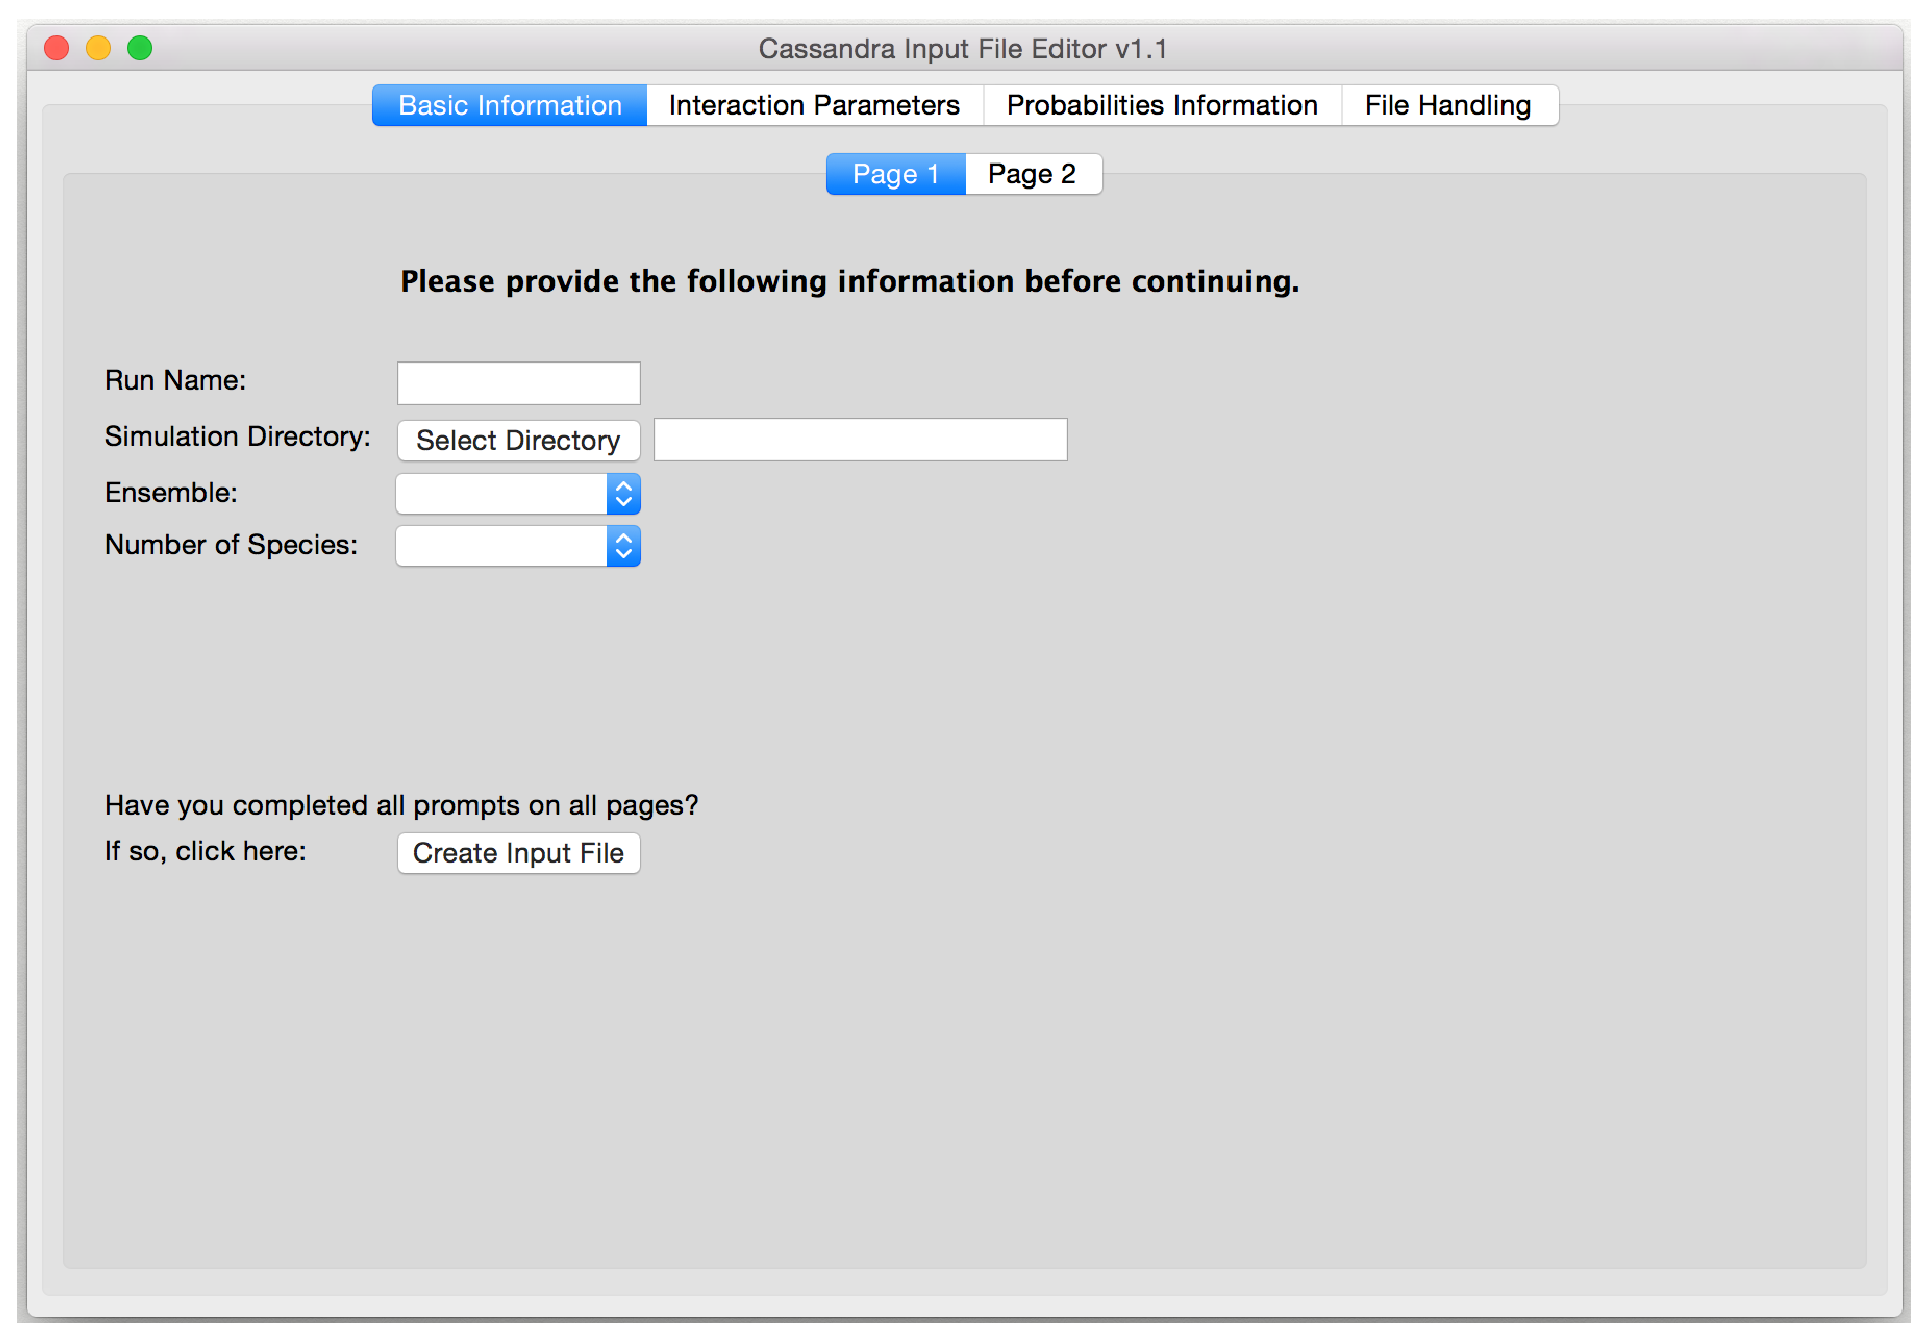
\includegraphics[width=\textwidth]{GUI_screenshot.eps}
 \caption{Cassandra Input File Graphical User Interface}
 \label{fig:GUIscreenshot}
\end{figure}

Complete all prompts as instructed on all panels of the GUI. 
Once all information has been provided, return to the Basic Information-Page 1 
section and click on ``Create Input File'' to create the input file. Note that if no 
value is entered for a required prompt, the GUI will inform the user 
via a KeyError message in the terminal.

If a given parameter is to be input at a later point in time, 
enter ``?'' and subsequently use a text editor to enter the 
desired value in the input file manually.  

If creating multiple input files, it is strongly encouraged to exit the GUI
and restart from the terminal each time a file is created, otherwise, data from the 
previous file may leak to the next file.

A set of executable files are provided that do not require the installation
of the wxPython module. These executables are available for Unix-like systems.
In order to run these, the user must change the access permissions of the executable through the
command \\ \\

\texttt{> chmod +x InputFileGUI\_v1\_1\_UNIX.exe}. 

Then, the user can execute the GUI by typing \\ \\
\texttt{> ./InputFileGUI\_v1\_1\_UNIX.exe}. 
\section{Generate an MCF file}
\label{sec:mcfgen}

The script \texttt{mcf\_gen.py} is a tool that aims to ease the setup of MCF files from scratch (see section \ref{sec:MCF_File} to learn more
about MCF files), as the generation of these files by hand can be error prone. 
In this section, a pentane MCF file will be generated to demonstrate the use of this tool.
The Transferable Potentials for Phase Equilibria (TraPPE) force field will be used to represent the pentane molecular interactions. 
This force field involves a pairwise-additive 12-6 Lennard-Jones potential to represent the dispersion-repulsion interactions. Additionally, bond angles and dihedral angles are represented through
harmonic and OPLS functional forms, respectively. Bond lengths are kept constant. The force field mathematical
expression becomes

\begin{align*}
U = \sum_{angles} K_\theta(\theta-\theta_0)^2 +
\sum_{dihedrals} \frac{1}{2}K_1[1+cos(\phi)]+\frac{1}{2}K_2[1-cos(2\phi)] + \frac{1}{2}K_3[1+cos(3\phi)]+\frac{1}{2}K_4[1-cos(4\phi)] + \\
\sum_{i} \sum_{i>j} 4 \epsilon_{ij} \left [  \left ( \frac {\sigma_{ij}} { r_{ij} }\right )^{12} - \left ( \frac {\sigma_{ij}} { r_{ij} }\right )^{6}\ \right ]
\end{align*}

First, generate (or obtain) a PDB file or a CML file. To generate a PDB or CML file, 
software such as Gaussview or Avogadro can be used. Alternatively, PDB files can
be downloaded from the internet (e.g. www.rcsb.org). In this example, a pentane PDB file using the 
program Gaussview v5.08 was be generated, as shown below. \\

%After launching the Gaussview interface, click on the ``Element Fragment'' button located on the upper-left corner of the
%window.
%
%
%\begin{figure}[h]
%\begin{center}
%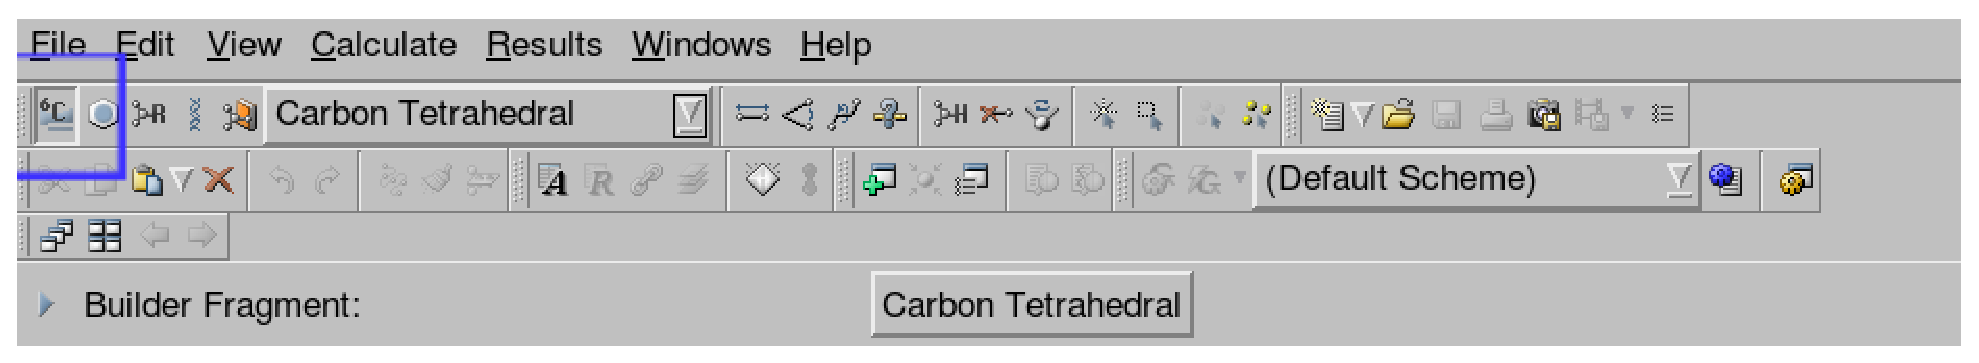
\includegraphics[height=1in]{gaussian1final.eps}
%\end{center}
%\end{figure}
%
%A periodic table will appear. Click on the ``Carbon'' button. 
%
%\begin{figure}[h]
%\begin{center}
%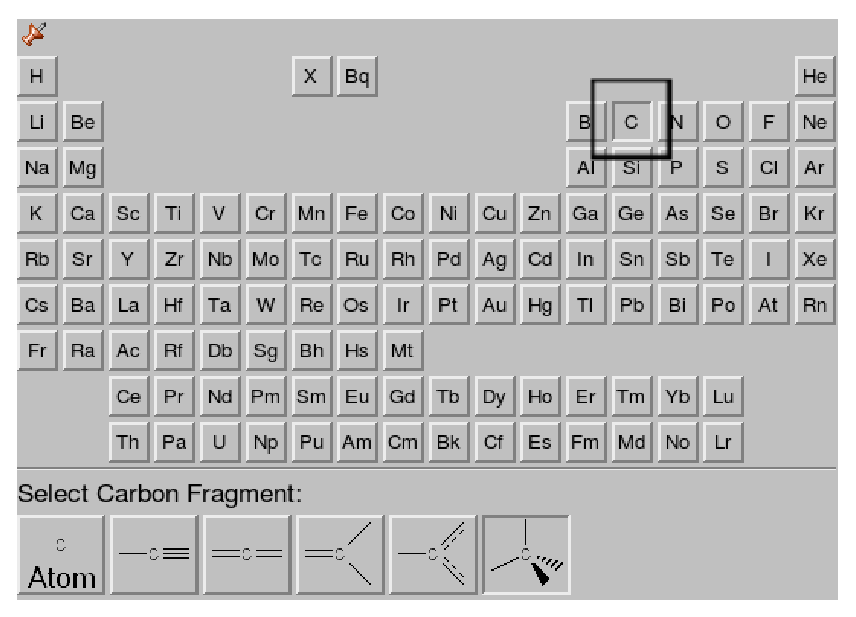
\includegraphics[height=3in]{gaussian2final.eps}
%\end{center}
%\end{figure}
%
%Click on the main workplace to insert the first $CH_4$ fragment.
%To increase the chain length, click on a hydrogen attached to the carbon. 
%
%\begin{figure}[h]
%\begin{center}
%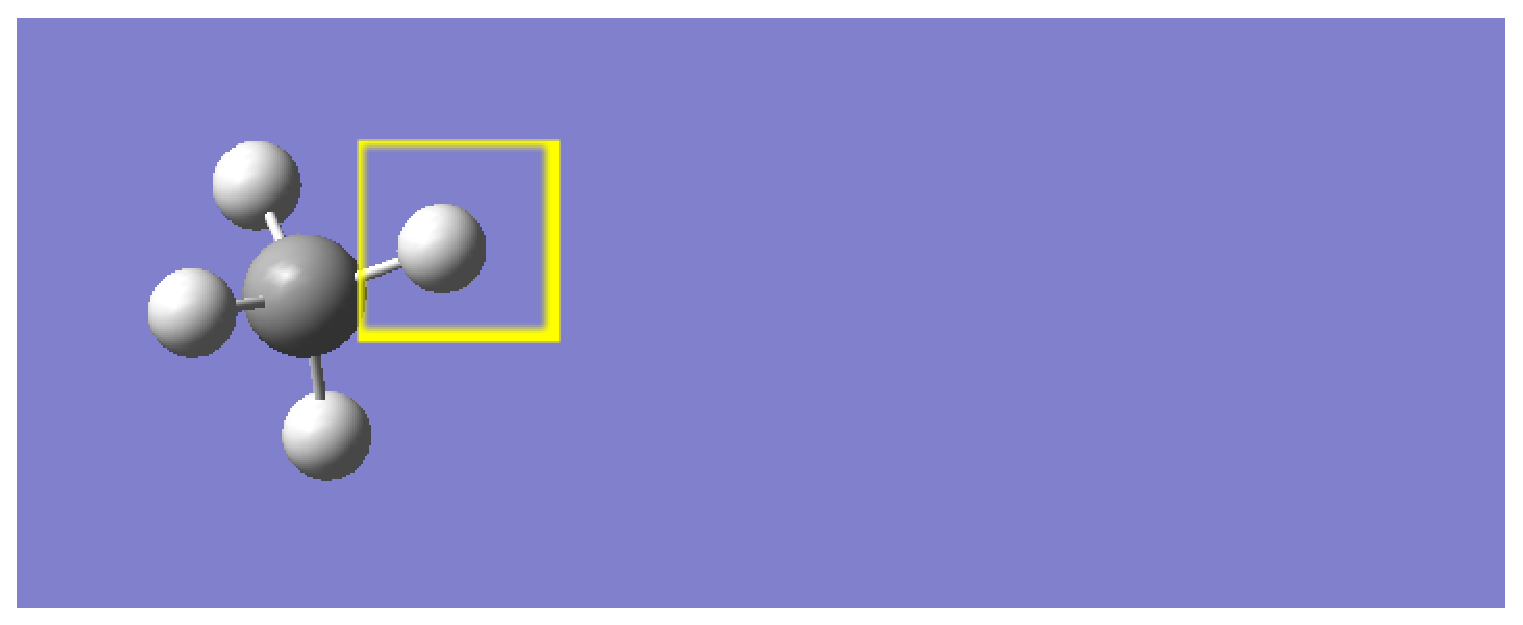
\includegraphics[height=2in]{gaussian3final.eps}
%\end{center}
%\end{figure}
%
%The final pentane structure should look something like this
%
%\begin{figure}[h]
%\begin{center}
%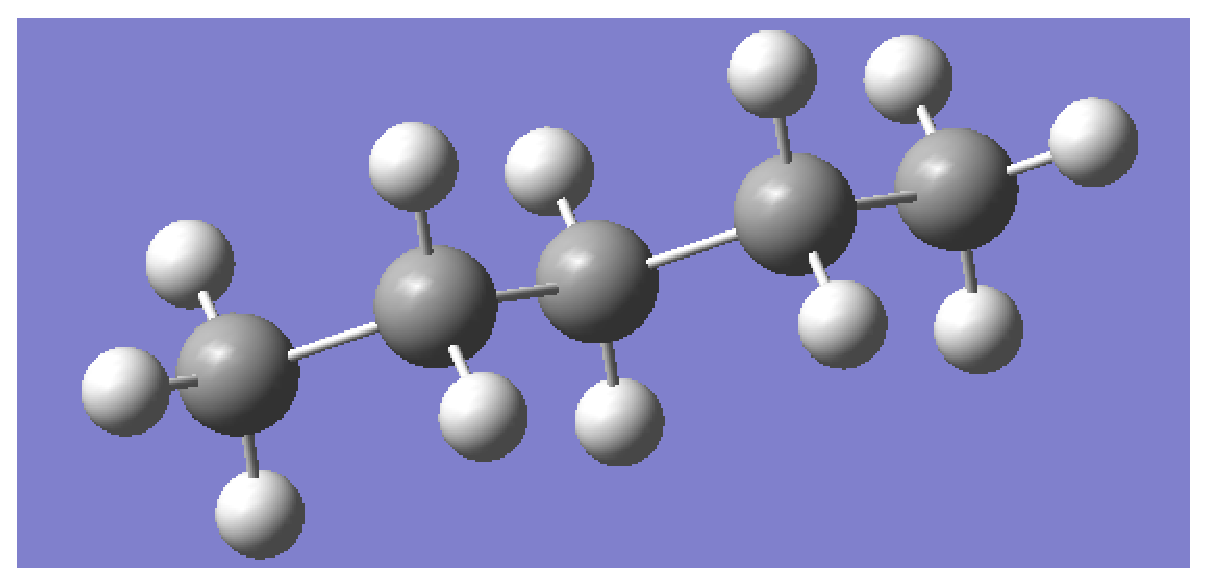
\includegraphics[height=2in]{gaussian4final.eps}
%\end{center}
%\end{figure}
%\vspace{3in}
%Right click on any place of the workplace, select the option builder and then
%select delete atoms.
%
%\begin{figure}[h]
%\begin{center}
%\includegraphics[height=2.5in]{gaussian5final.eps}
%\end{center}
%\end{figure}
%
%Click on all the hydrogen atoms to delete them 
%
%\begin{figure}[h]
%\begin{center}
%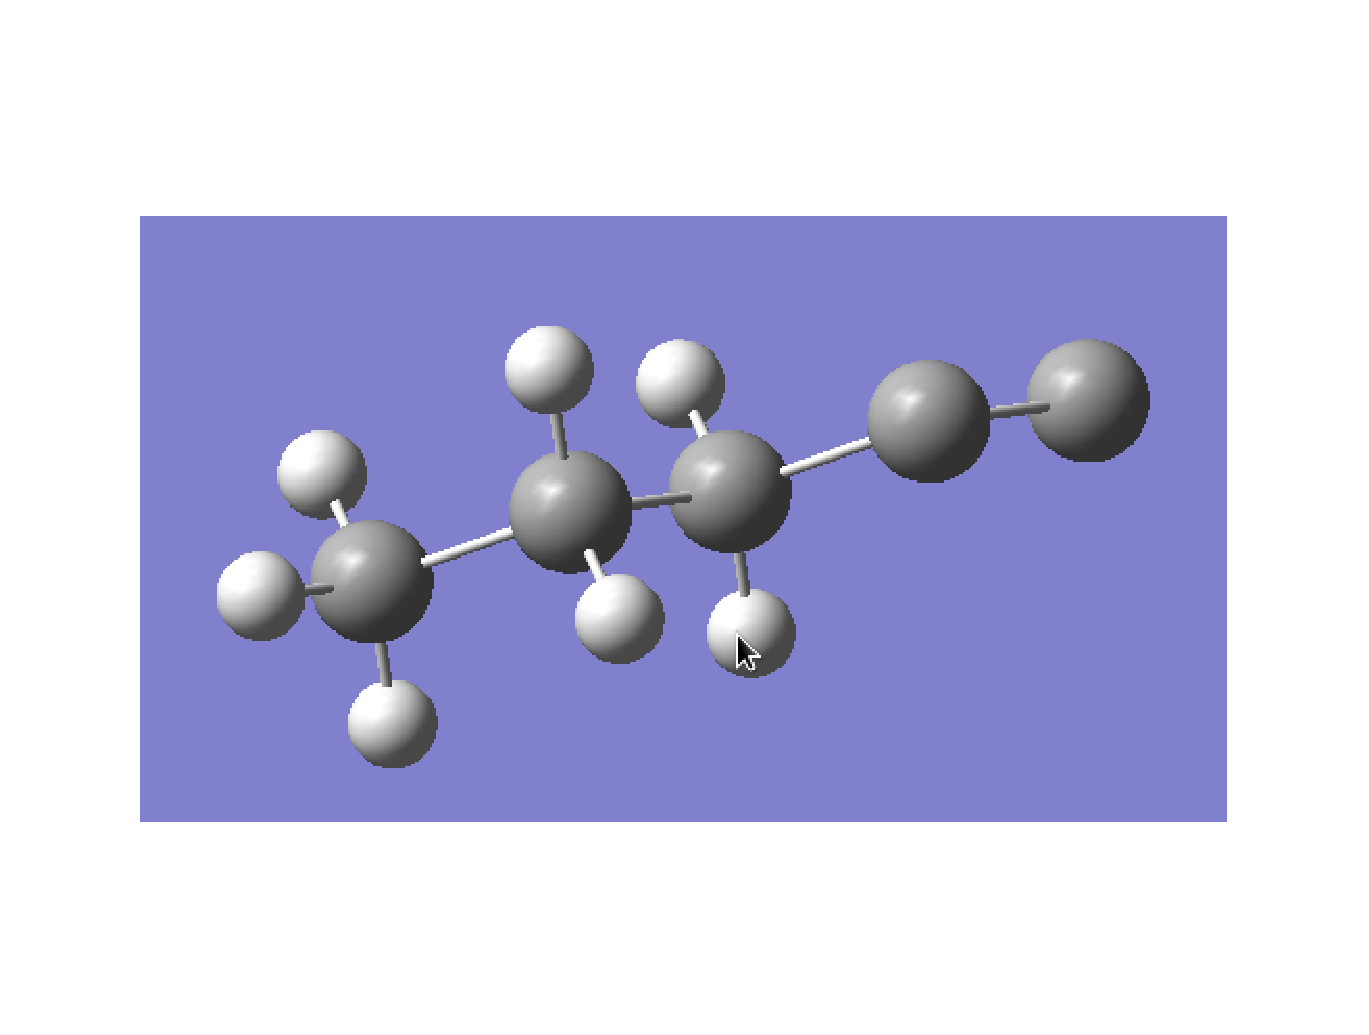
\includegraphics[height=2.5in]{gaussian7final.eps}
%\end{center}
%\end{figure}
%
%\vspace{3in}
%Go back to main menu, click on File - Save.
%
%\begin{figure}[h]
%\begin{center}
%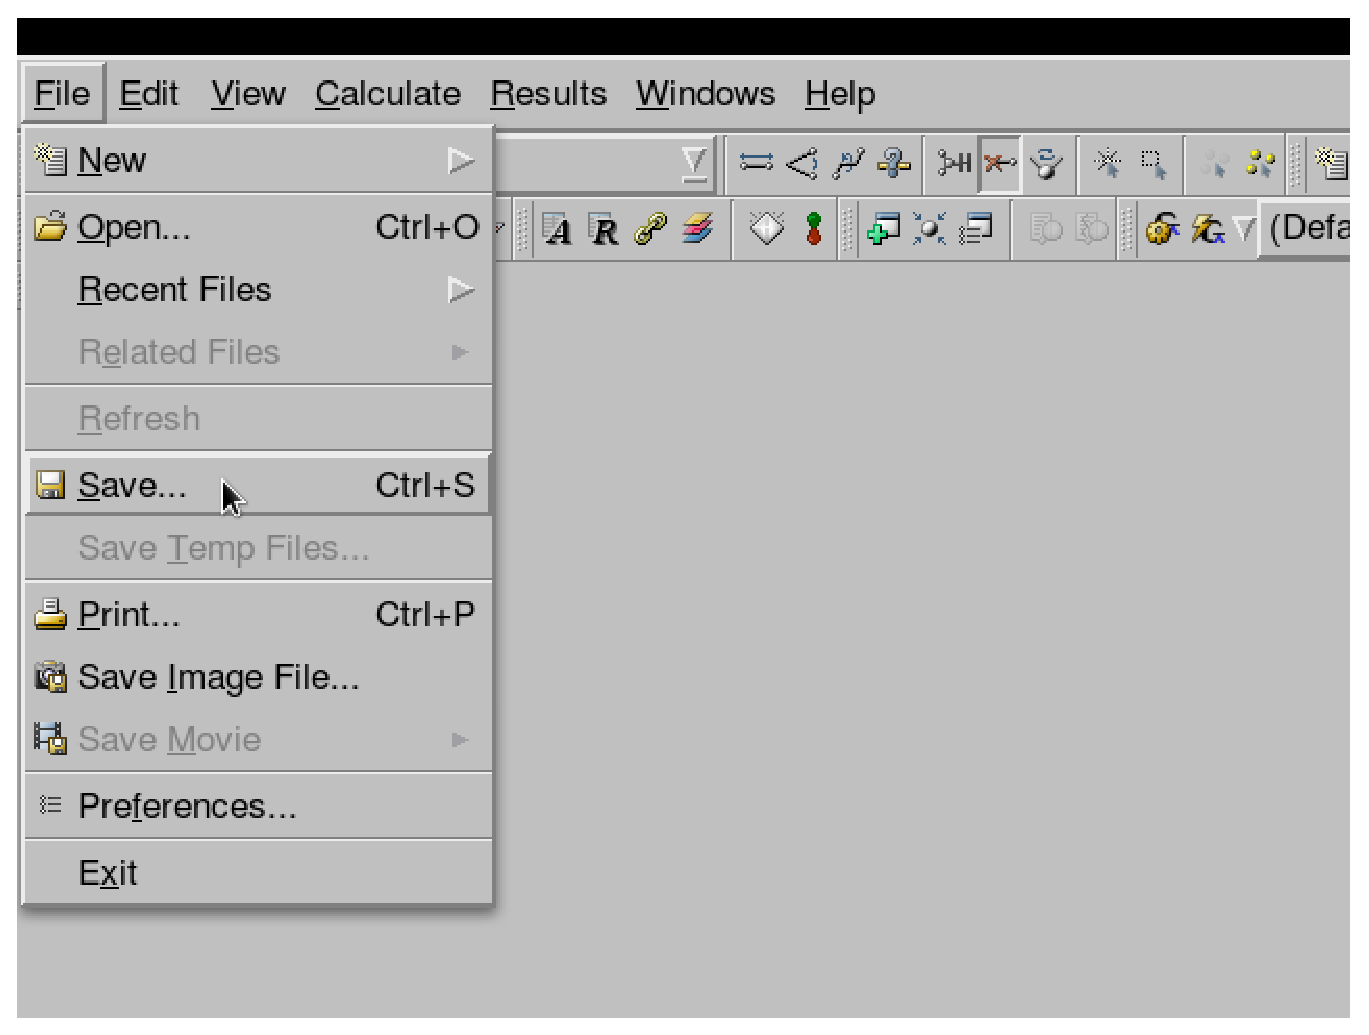
\includegraphics[height=2.5in]{gaussian8final.eps}
%\end{center}
%\end{figure}
%
%Type the name of the file and select PDB as the file type from the bottom menu.
%
%\begin{figure}[h]
%\begin{center}
%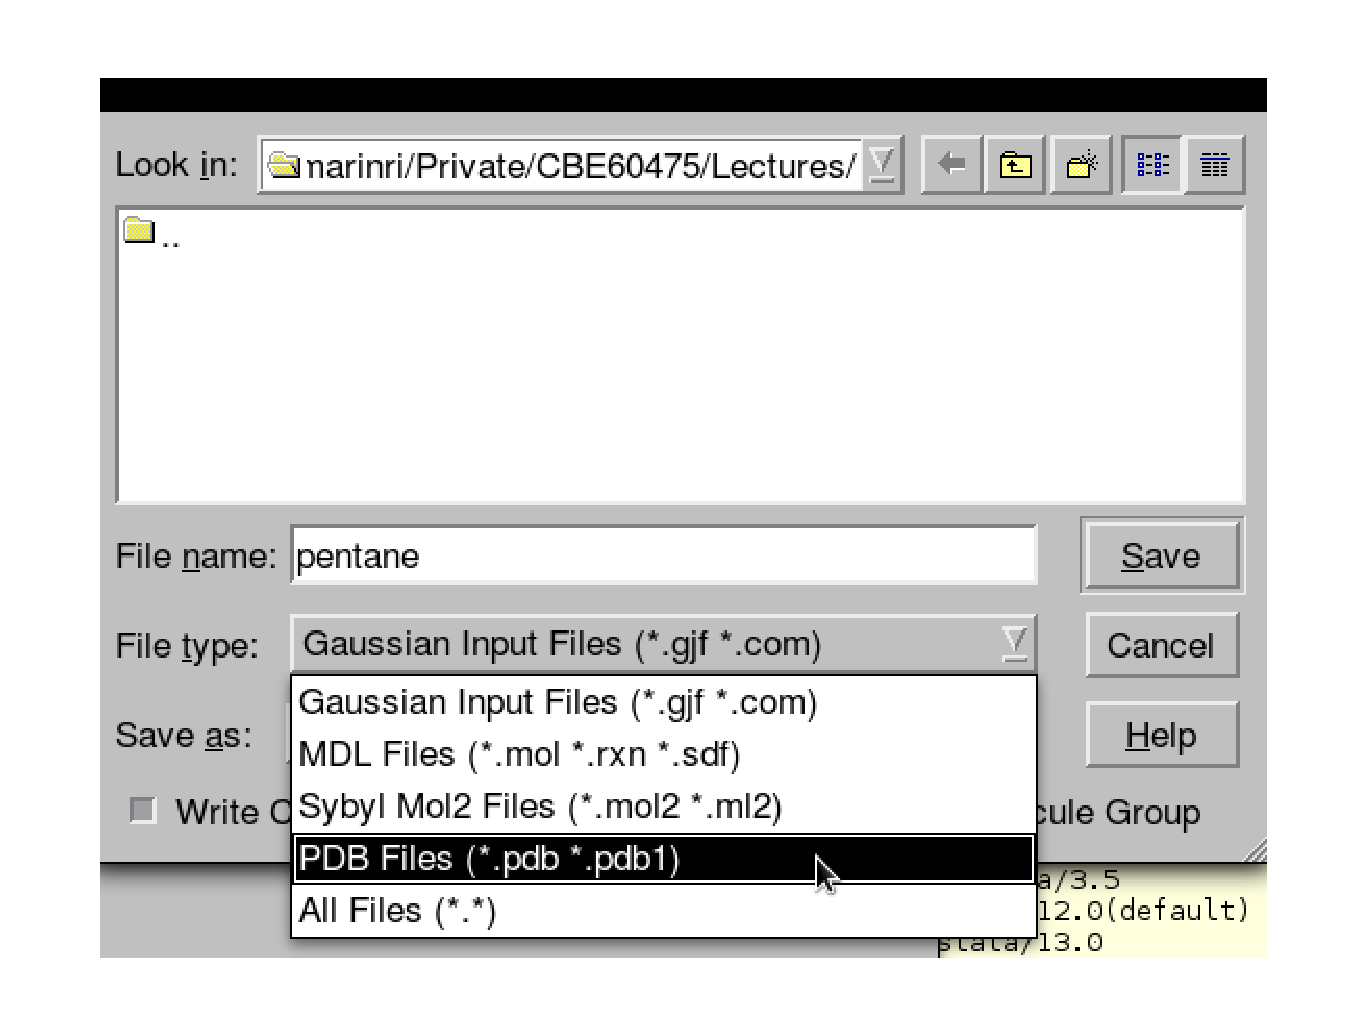
\includegraphics[height=2.5in]{gaussian9final.eps}
%\end{center}
%\end{figure}
%
%\vspace{3in}
%Close Gaussview. Back in the terminal, open the PDB file using your favorite text editor.

\begin{figure}[h]
\begin{center}
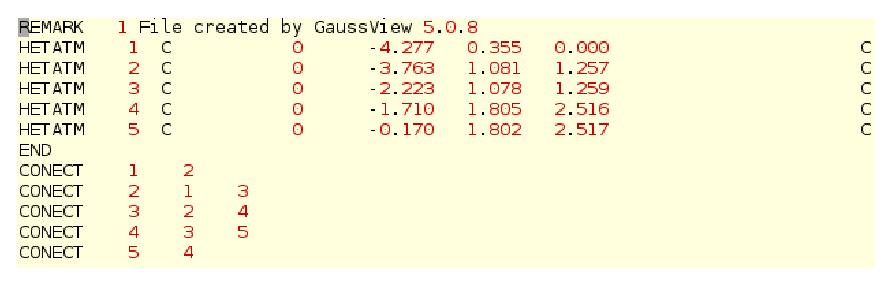
\includegraphics[height=1in]{pdbfile_final.eps}
\end{center}
\end{figure}

Append a column containing the atom types.

\begin{figure}[h]
\begin{center}
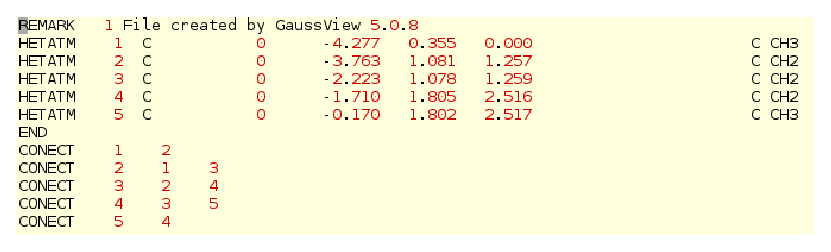
\includegraphics[height=1in]{pdbfile_edited_final.eps}
\end{center}
\end{figure}

Avogadro v1.1.1 can also be used to generate CML files. Below is an example of a 
CML file generated using Avogadro

\begin{figure}[h]
\begin{center}
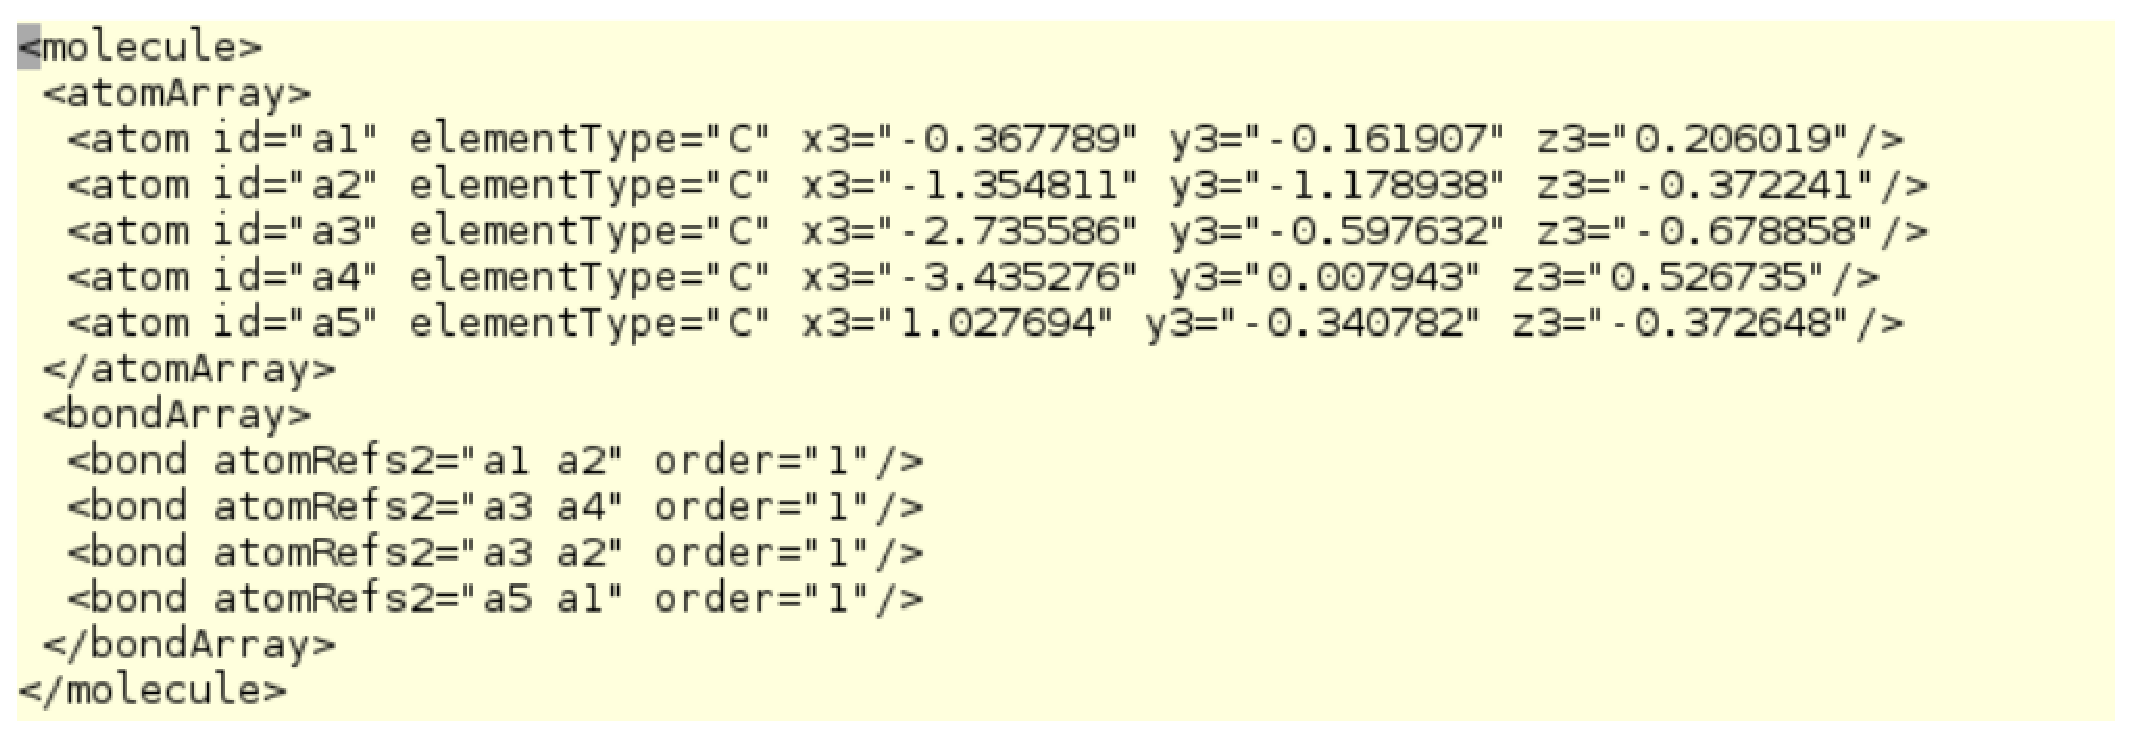
\includegraphics[height=1.5in]{pentane_cml.eps}
\end{center}
\end{figure}

\vspace{3in}
Modify the pentane united atom CML file. Note that the atom type is appended as a last
column between quotation marks.

\begin{figure}[h]
\begin{center}
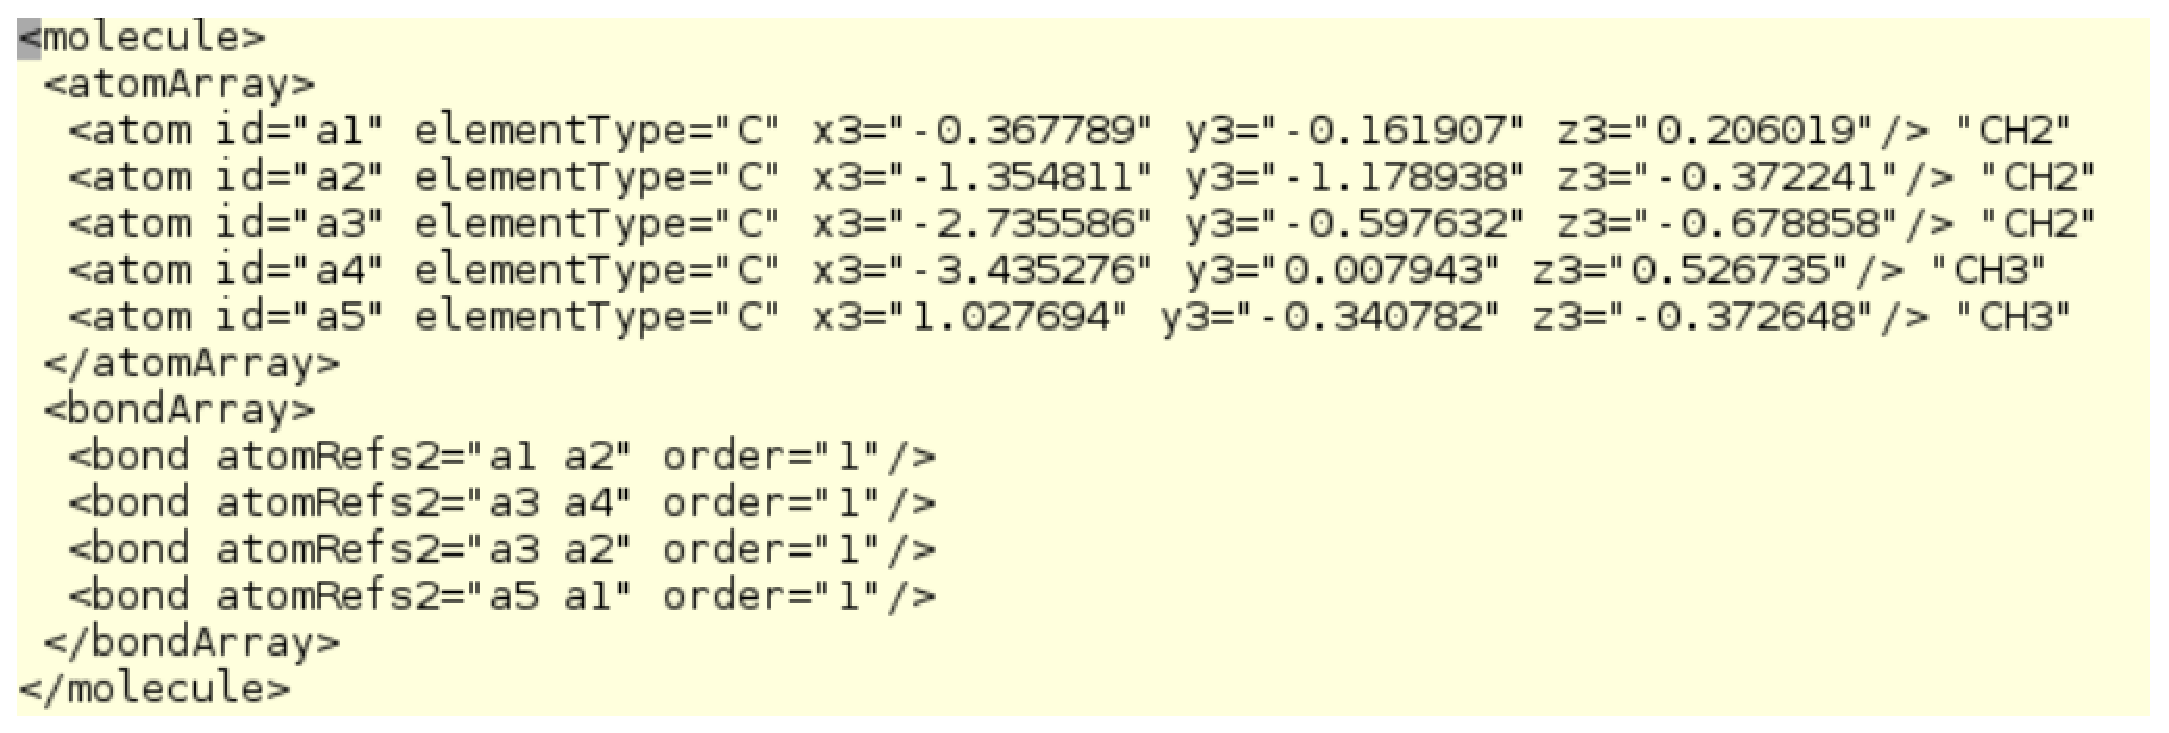
\includegraphics[height=1.5in]{pentane_cml_modified.eps}
\end{center}
\end{figure}

In the terminal, run the following command:\\ \\
\texttt{>python mcfgen.py pentane.pdb --ffTemplate}

This command will create an .ff file. The first three sections of the FF file are displayed next. 
Do not modify these.

\begin{figure}[h]
\begin{center}
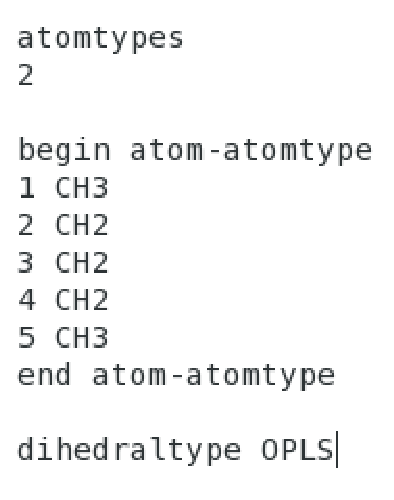
\includegraphics[height=2in]{top_ff.eps}
\end{center}
\end{figure}

The force field parameters for non-bonded (not shown), bonded, angle, dihedral (not shown)
and coulombic interactions (not shown) must be entered next to the corresponding keyword.
For example, the angle type CH3 CH2 CH2 has an angle of 114.0. This value must be placed
next to the ``Angle'' keyword.

\begin{figure}[h]
\begin{center}
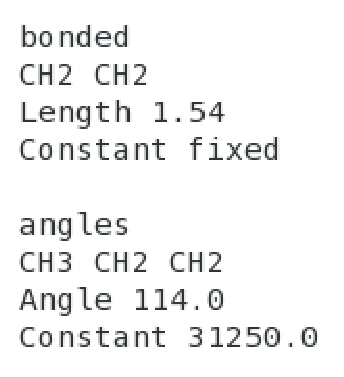
\includegraphics[height=1.5in]{body_ff.eps}
\end{center}
\end{figure}

\vspace{3in}
For more examples of filled ff files, please refer to the examples contained in the /Scripts/MCF\_Generation/ directory. Using the
filled .ff file, run: \\

\texttt{> python mcfgen.py pentane.pdb} \\

Check the file newly created pentane.mcf for any possible errors. This example can be found in the directory 
/Scripts/MCF\_Generation/PDB/

\section{Generate library of fragment configurations}
\label{sec:libgen}

The goal of the script \texttt{library\_setup.py} is to automate the generation of fragment libraries.
As a starting point, the script requires the simulation input file, and the MCF and PDB 
files for each of the species. To run this script, type \\

\texttt{> library\_setup.py \$PATH\$/cassandra.exe input\_file.inp pdbfilespecies1.pdb pdfilespecies2.pdb ...} \\

This script will create the necessary files to create the fragment libraries. It will also run Cassandra 
to generate these libraries, whose location will be at \\

\texttt{/species?/frag?/frag?.inp} \\

where '?' refers to the species number, for example, species 1, species 2 etc. \\

Note that the script overwrites the section of the input file where 
needed (i.e. \# Frag\_Info) with the aforementioned directory locations.

\chapter{Simulating Rigid Solids and Surfaces}

Simulations involving a rigid solid or surface can be performed in constant volume ensembles
(i.e., NVT and GCMC). 
For example, an adsorption isotherm can be computed with a GCMC simulation in which fluid molecules
are inserted into a crystalline solid.
In addition to the files described in Chapter \ref{ch:input_files}, 
the following files are required to run a simulation with a rigid solid or surface:

\begin{itemize}
\item a molecular connectivity file with force field parameters for each atom in the solid (*.mcf)
\item a fragment library file listing the coordinates of each atom in the solid (*.dat)
\item a configuration file with the initial coordinates of the all atoms in the system (*.xyz) 
\end{itemize} 

The MCF and fragment library file can be created using the scripts discussed in Sections \ref{sec:mcfgen} and \ref{sec:libgen}. 
Each of these scripts requires a starting PDB configuration file.
The input file also requires specific parameters as given in the following section. Sample input scripts for GCMC simulations
of various fluids in silicalite are included in the Examples/GCMC directory of the Cassandra distribution.
 
\section{Input file}
The input file should be completed as described in Section \ref{sec:Input_File}, but with the following parameters:

\begin{itemize}
	\item Under the keyword \texttt{\# Prob\_Translation}, the translation width for the solid is 0.
	\item Under the keyword \texttt{\# Prob\_Rotation}, the rotation width for the solid is 0.
	\item Under the keyword \texttt{\# Prob\_Regrowth}, the regrowth probability for the solid is 0.
	\item The volume dimensions under the keyword \texttt{\# Box\_Info} must match the crystal dimensions.
	\item Under the keyword \texttt{\# Start\_Type}, the \texttt{read\_config} or \texttt{add\_to\_config} options must be used.
\end{itemize}

GCMC simulations require the following additional parameters:

\begin{itemize}
	\item Under the keyword \texttt{\# Prob\_Insertion} insertion method for the solid is \texttt{none}.
	\item Under the keyword \texttt{\# Chemical\_Potential\_Info}, no chemical potential is required for the solid.
\end{itemize}

\section{PDB file}\label{sec:solid_pdb}
A PDB configuration file for a zeolite can be created in the following ways, among others: 

\begin{itemize}
	\item Manually, with atomic coordinates from the literature. 
	For example, the atomic coordinates of silicalite are published in Ref. \cite{Meier:1981}.

	\item From a Crystallographic Information File (CIF), which can be downloaded from
	the Database of Zeolite Structures (http://www.iza-structure.org/databases/).
	From the home page, click on the menu "Framework Type" and select your zeolite. 
	The website will display structural information about the zeolite and will have 
	a link to download a CIF. The CIF contains information about the 
	zeolite structure such as cell parameters, space groups, T and O atom coordinates. 
	A CIF can be converted into a PDB file using either Mercury or VESTA, both of which
	are available to download for free.
	For example, using VESTA:

	\begin{enumerate}
		\item From the File menu, click Open. Then download the CIF (e.g. MFI.cif)

		\item From the Objects menu, click Boundary. Enter the desired number of replicas
		along each axis. To output a single unit cell, enter -0 to 1 in the x, y and z ranges. 
		To output a 2x2x2 crystal, enter -1 to 1 in the x, y and z ranges. 

		\item From the File menu, click Export Data. Enter a filename ending with .pdb (e.g. MFI.pdb)
	\end{enumerate}

\end{itemize}

Executing the script \texttt{mcfgen.py} for solids involves using the 
\texttt{-s} or \texttt{--solid}. This will skip the CONECT information
that might be present in PDB files of solid materials, and thus
skip creating connectivity information such as bonds, angles, 
dihedrals and fragments.

\section{Molecular connectivity file}\label{sec:solid_mcf}
Since the solid structure will be rigid, no bond distances, angle parameters or dihedral parameters are needed in the MCF.
The PDB file for the rigid solid does not list CONECT information, so the \texttt{mcfgen.py} script will not include bond, 
angle, or dihedral sections in the force field template (*.ff) or MCF. The number of fragments will be zero. 
Only nonbonded parameters are needed.

\section{Fragment library files}\label{sec:fragment file}
The \texttt{library\_setup.py} script will not create a fragment library since the MCF lists zero fragments.

\section{Configuration xyz file}\label{sec:solid_xyz}
A simulation is initiated from an xyz file using the \texttt{read\_config} or \texttt{add\_to\_config} options. 
Section \ref{sec:Start_Type} details the \texttt{read\_config} and \texttt{add\_to\_config} options.

\chapter{Implementing the Metropolis Acceptance Criteria}

All Monte Carlo moves are implemented in Cassandra to preserve detailed balance between each pair of microstates $m$ and $n$
\begin{equation}
\label{eq:detailedBalance}
\Pi_{mn}\ \alpha_{mn}\ p_m = \Pi_{nm}\ \alpha_{nm}\ p_n
\end{equation}
where $\Pi_{mn}$ is the probability of accepting the move from microstate $m$ to microstate $n$, $\alpha_{mn}$ is the probability of attempting the move that will form $n$ from $m$, and $p_m$ is the probability of $m$ in the ensemble of interest.

In Cassandra, detailed balance is enforced via the Metropolis criterion
\begin{equation}
\label{eq:metropolis}
\Pi_{mn} = \min\left(1, \frac{\alpha_{nm}}{\alpha_{mn}} \frac{p_n}{p_m} \right)
\end{equation}
The ratio in Eq.\ (\ref{eq:metropolis}) will often involve an exponential, e.g. $e^{-\beta \Delta U}$. To preserve precision in the energy calculation, the acceptance probability is computed
\begin{equation}
\label{eq:metropolis_2}
\Pi_{mn} = \exp\left\{-\max\left[0, \ln\left(\frac{\alpha_{mn}}{\alpha_{nm}} \frac{p_m}{p_n}\right)\right]\right\}
\end{equation}
The logarithm, defined in code as ln\_pacc, is tested in the function accept\_or\_reject() which is defined in file accept\_or\_reject.f90. If ln\_pacc is greater than 0 and less than a maximum numerical value, $\Pi_{mn}$ is computed and compared to a random number.

\begin{minipage}{\linewidth}
\begin{lstlisting}[firstnumber=47, caption=accept\_or\_reject.f90]
  accept = .FALSE.

  IF (ln_pacc <= 0.0_DP) THEN

     accept = .TRUE.

  ELSE IF ( ln_pacc < max_kBT) THEN

     pacc = DEXP(-ln_pacc)

     IF ( rranf() <= pacc ) THEN
         
        accept = .TRUE.

     END IF

  END IF
\end{lstlisting}
\end{minipage}

\section{Canonical Monte Carlo}
\label{sec:NVT}
In the canonical ensemble, the number of molecules $N$, the volume $V$ and temperature $T$ are all constant. The position, orientation and conformation of a semi-flexible molecule with fixed bond-lengths containing $M$ atoms is given by a 2$M$+1-dimensional vector $\mathbf{q}$. The positions, orientations and conformations of all $N$ molecules are denoted $\mathbf{q}^N$.

The probability of observing microstate $m$ with configuration $\mathbf{q}_m^N$ is
\begin{equation}
\label{eq:pNVT}
p_m = \frac{e^{-\beta U\left(\mathbf{q}_m^N\right)}}{Z(N,V,T)}\ d\mathbf{q}^N
\end{equation}
where $\beta$ is the inverse temperature $1/k_BT$, $U$ is the potential energy, the differential volume $d\mathbf{q}^N$ is included to make $p_m$ dimensionless and $Z$ is the configurational partition function
\begin{equation}
\label{eq:configPartitionFn_NVT}
Z(N,V,T) = \int e^{-\beta U(\mathbf{q}^N)} d\mathbf{q}^N.
\end{equation}
The integral is over all $N(2M+1)$ degrees of freedom. The ratio of microstate probabilities follows from Eq.\ (\ref{eq:pNVT})
\begin{align}
\label{eq:pNVT_ratio}
\frac{p_m}{p_n} &= \frac{e^{-\beta U\left(\mathbf{q}_m^N\right)} d\mathbf{q}^N/Z(N,V,T)}{e^{-\beta U\left(\mathbf{q}_n^N\right)} d\mathbf{q}^N/Z(N,V,T)} \nonumber \\
&= e^{\beta (U_n - U_m)} = e^{\beta \Delta U}
\end{align}
The configurational partition function $Z$ and differential volume $d\mathbf{q}^N$ both cancel, leaving only the ratio of Boltzmann factors.

New configurations are generated by attempting moves that translate, rotate and regrow a randomly selected molecule.

\subsection{Translating a Molecule}
\label{sec:translate}
A molecule is translated by moving its center of mass in each Cartesian direction by a random amount chosen from the uniform distribution on the interval [-$\delta r_{max},\delta r_{max}$]. The maximum displacement $\delta r_{max}$ must be given in the input file. The translation move is symmetric in forward and reverse directions. That is, either microstate $n$ can be formed from microstate $m$ and vice versa by moving one molecule within $\delta r_{max}$ in each Cartesian direction, or microstate $n$ cannot be formed at all. As a result, $\alpha_{mn} = \alpha_{nm}$.

The acceptance probability for a translation move follows from Eq.\ (\ref{eq:pNVT_ratio})
\begin{equation}
\label{eq:pAcc_translate}
\ln \left( \frac{\alpha_{mn}}{\alpha_{nm}} \frac{p_m}{p_n} \right) = \ln \left( \frac{p_m}{p_n} \right) = \beta \Delta U
\end{equation}

In Cassandra, the translation move is implemented in the subroutine Translate defined in translate.f90. The relevant lines from version 1.1 are quoted below. The variable names in the translate.f90 code are identified with the symbols from Eq.\ (\ref{eq:pAcc_translate}) in Table \ref{table:translate}.

\begin{lstlisting}[firstnumber=274, caption=translate.f90, label=code:translate]
ln_pacc = beta(this_box) * delta_e
accept = accept_or_reject(ln_pacc)
\end{lstlisting}

\begin{table}
\caption{Variable symbols and code names for translating and rotating a molecule}
\label{table:translate}
\centering
\begin{tabular}{|c|c|} \hline
 {\bf Symbol} & {\bf Code name} \\ \hline
 $\beta$ & beta(this\_box) \\
 $\Delta U$ & delta\_e \\
 \hline
\multicolumn{2}{c}{}
\end{tabular}
\end{table}

\subsection{Rotating a Molecule}
\label{sec:rotate}
A linear molecule is rotated differently than a nonlinear molecule. A molecule is identified as linear if it is composed of 2 atoms or if all the angles are rigid with a bond angle of 180$\degree$. If the molecule is linear: 

\begin{enumerate}
	\item Pick three random angles: $\phi$ on [$-\pi,\pi$], $\cos(\theta)$ on [-1,1], and $\psi$ on [$-\pi,\pi$].
	\item With the origin at the molecule's center of mass, rotate by $\phi$ around $z$, rotate by $\theta$ around $x'$, and rotate by $\psi$ around $z'$, as shown in Fig. \ref{fig:EulerAngles}.
\end{enumerate}

Even though three angles are randomly chosen, the probability of the resulting orientation is $d\cos(\theta)d\phi/4\pi$.

\begin{figure}[h]
	\centering
	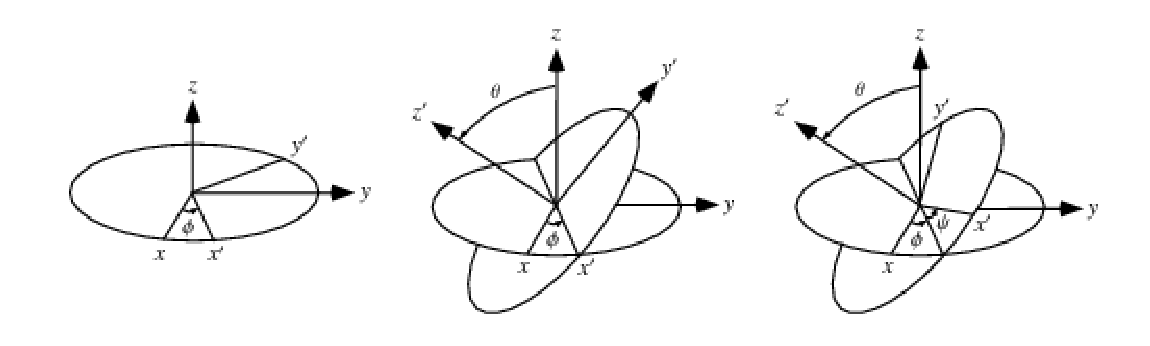
\includegraphics[width=0.9\textwidth]{EulerAngles.eps}
	\caption{Procedure for rotating linear molecules. \newline Image from mathworld.wolfram.com/EulerAngles.html.}
	\label{fig:EulerAngles}
\end{figure}

If the molecule is nonlinear:

\begin{enumerate}
	\item Randomly select an axis: $x$, $y$, or $z$.
	\item Choose a random angular displacement $\delta \theta$ from $[-\delta \theta_{max}, \delta \theta_{max}]$. $\delta \theta_{max}$ must be given in the input file.
	\item Rotate the molecule around a vector parallel to the selected axis and through its center of mass by $\delta \theta$.
\end{enumerate}

In either case, the rotation move is symmetric, $\alpha_{mn} = \alpha_{nm}$, and the acceptance criteria is given by Eq.\ (\ref{eq:pAcc_translate}). The rotation move is implemented in subroutine Rotate defined in rotate.f90.

\begin{lstlisting}[firstnumber=261, caption=rotate.f90, label=code:rotate]
ln_pacc = beta(this_box) * delta_e
accept = accept_or_reject(ln_pacc)
\end{lstlisting}

\subsection{Regrowing a Molecule}
\label{sec:regrow}
Internal degrees of freedom in flexible molecules are sampled by deleting one or more fragments from the molecule and replacing the deleted fragments with conformations from a reservoir of fragment conformations. If the molecule consists of only a single fragment (e.g, water, all atom methane, united atom propane, all atom cyclohexane), the entire molecule is deleted and replaced as follows:

\begin{enumerate}
	\item Randomly select a molecule $i$ with uniform probability $1/N$, record its center-of-mass position and delete it.
	\item Select a molecular conformation with Boltzmann probability $e^{-\beta U(\mathbf{q}_{int,n}^{(i)})}/Z_{int}$, where $\mathbf{q}_{int,n}^{(i)}$ are the internal bond or improper angles of molecule $i$ in microstate $n$ and $Z_{int}$ is the configurational partition function over internal degrees of freedom (see Eq. (\ref{eq:configPartitionFn_1VT})).
	\item Pick three random angles: $\phi$ on [$-\pi,\pi$], $\cos(\theta)$ on [-1,1], and $\psi$ on [$-\pi,\pi$]. Rotate the molecule as shown in Fig. \ref{fig:EulerAngles}. The probability of the resulting orientation is $d\mathbf{q}_{rot}/Z_{rot}$, which for a nonlinear molecule is $d\cos(\theta) d\phi d\psi / 8 \pi^2$.
	\item Place the molecule with the selected conformation and orientation at the same center-of-mass position as the deleted molecule.
\end{enumerate}

Regrowing a monoatomic particle has no effect. Regrowing a linear molecule is the same as rotating it. The overall probability $\alpha_{mn}$ of regrowing a molecule with the selected orientation and conformation is 

\begin{equation}
\label{eq:alpha_regrow}
\alpha_{mn} = \frac{1}{N} \frac{d\mathbf{q}_{rot}}{Z_{rot}} \frac{e^{-\beta U(\mathbf{q}_n^{(i)})}d\mathbf{q}_{int}}{Z_{int}}
\end{equation}

where $\mathbf{q}_n^{(i)}$ denotes the position, orientation and conformation of molecule $i$ in microstate $n$ and $U(\mathbf{q}_n^{(i)})$ is the potential energy of the isolated molecule $i$, i.e. the intramolecular potential energy. The reverse probability $\alpha_{nm}$ is identical except for the intramolecular potential energy $U(\mathbf{q}_m^{(i)})$ of molecule $i$ in microstate $m$. Using Eqs. (\ref{eq:pNVT_ratio}) and (\ref{eq:alpha_regrow}), the acceptance criteria for the regrowth of a single fragment molecule is

\begin{align}
\label{eq:pAcc_regrow}
\ln\left( \frac{\alpha_{mn}}{\alpha_{nm}} \frac{p_m}{p_n} \right) &= \beta \left[\left(U(\mathbf{q}^N_n) - U(\mathbf{q}^N_m)\right) - \left( U(\mathbf{q}_n^{(i)}) - U(\mathbf{q}_m^{(i)})\right)\right] \\ \nonumber
&= \beta \Delta U - \beta \Delta U_{int}^{(i)} = \beta \Delta U_{inter}^{(i)}
\end{align}

Only the change in the intermolecular potential energy between molecule $i$ and the other $N-1$ molecules contributes to the acceptance criteria. The code that implements Eq. (\ref{eq:pAcc_regrow}) is shown in Code \ref{code:cbmcRegrow} in Section \ref{sec:cbmcRegrow}.

If the molecule consists of more than one fragment (e.g., all atom ethane, all atom toluene, united atom butane), a bond is cut and the severed fragments are regrown using Configurational Bias Monte Carlo (CBMC). See Section \ref{sec:cbmcRegrow} for more details.

\subsection{Canonical Partition Function}
In Sections \ref{sec:translate}-\ref{sec:rotate}, the microstate probability is normalized by the configuration partition function $Z$ because the only relevant degrees of freedom are configurational. In other ensembles, the full partition function $Q$ appears, integrated over both configuration space $\mathbf{q}^N$ and momenta space $\mathbf{p}_q^N$

\begin{equation}
\label{eq:partitionFn_NVT}
Q(N,V,T) = \frac{1}{h^{N(2M+1)} N!} \int e^{-\beta H(\mathbf{p}_q^N, \mathbf{q}^N)}\ d\mathbf{p}_q^N d\mathbf{q}^N
\end{equation}

where the 2$M$+1 momenta $\mathbf{p}_q$ are conjugate to the generalized coordinates $\mathbf{q}$. The momenta and configuration integrals are separable, and the single molecule momenta integrals are all identical.

\begin{align}
Q(N,V,T) &= \frac{1}{N!} \left[\int e^{-\beta U(\mathbf{q}^N)} d\mathbf{q}^N \right] \left[\frac{1}{h^{2M+1}} \int e^{-\beta K(\mathbf{p}_q)}\ d\mathbf{p}_q \right]^N \nonumber \\
&= \frac{1}{N!} Z(N,V,T) \left[\frac{Q(1,V,T)}{Z(1,V,T)}\right]^N
\end{align}

where $Q(1,V,T)$ is the partition function of a single molecule in a box. The center of mass integrals for a single molecule are separable from the integrals over rotational and internal degrees of freedom:

\begin{equation}
\label{eq:partitionFn_1VT}
Q(1,V,T) = Q_{com}Q_{rot+int} = V \Lambda^{-3} Q_{rot+int}
\end{equation}

where $\Lambda$ is the de Broglie wavelength of the molecule and the rotational and internal momenta integrals in $Q_{rot+int}$ are not separable since the moments of inertia will depend on the conformation adopted by the molecule. The configurational partition function is further separable into center of mass (translational), orientational and internal degrees of freedom:

\begin{equation}
\label{eq:configPartitionFn_1VT}
Z(1,V,T) = VZ_{rot}Z_{int}
\end{equation}

where the volume $V$ is the translational partition function and $Z_{rot}$ equals 4$\pi$ for a linear molecule and 8$\pi^2$ for a nonlinear molecule.

\section{Isothermal-Isobaric Monte Carlo}
\label{sec:NPT}
In the isothermal-isobaric ensemble, the number of particles $N$, the pressure $P$ and temperature $T$ are all constant while the volume $V$ and energy $E$ fluctuate. The partition function is

\begin{equation}
\label{eq:partitionFn_NPT}
\Delta(N,P,T) = \int e^{-\beta P V} Q(N,V,T) dV
\end{equation}

Note that $Q$ is dimensionless and $\Delta$ has dimensions of volume. The probability of the system having volume $V$ is 

\begin{equation}
\label{eq:pV}
p(V) = \frac{Q(N,V,T)e^{-\beta P V}}{\Delta(N,P,T)}dV
\end{equation}

The probability of observing microstate $m$ with configuration $\mathbf{q}_m^N$ and volume $V_m$ is

\begin{align}
\label{eq:pNPT}
p_m &= \frac{e^{-\beta U(\mathbf{q}_m^N)}d\mathbf{q}_m^N}{Z(N,V_m,T)}\ \frac{Q(N,V_m,T) e^{-\beta P V_m} dV}{\Delta(N,P,T)} \nonumber \\
&= \frac{e^{-\beta U_m - \beta P V_m}}{\Delta(N,P,T)}\ \left(\frac{Q(1,V_m,T)}{Z(1,V_m,T)}\ d\mathbf{q}_m\right)^N dV
\end{align}

where the differential volume element $d\mathbf{q}_m^N$ has subscript $m$ becuase it depends on the volume $V_m$. The ratio of microstate probabilities is

\begin{equation}
\label{eq:pNPT_ratio}
\frac{p_m}{p_n} = e^{\beta (U_n - U_m) + \beta P (V_n - V_m)} \left(\frac{d\mathbf{q}_m}{d\mathbf{q}_n}\right)^N = e^{\beta \Delta U + \beta P \Delta V} \left(\frac{d\mathbf{q}_m}{d\mathbf{q}_n}\right)^N
\end{equation}

\subsection{Scaling the Volume}
\label{subsec:scaling_the_volume}
In Cassandra, new volumes are sampled as follows:

\begin{enumerate}
	\item Pick a random volume $\Delta V$ with uniform probability from the interval [$-\delta V_{max}$,\ $\delta V_{max}$]. The trial volume is $V + \Delta V$.
	\item Scale the box lengths uniformly.
	\item Scale the center of mass of each molecule uniformly.
\end{enumerate}

The probability of selecting $\Delta V$ is the same as selecting $-\Delta V$ which makes scaling the volume symmetric, $\alpha_{mn}=\alpha_{nm}$. Scaling the configurations changes the differential element $d\mathbf{q}_m^N$ surrounding configuration $\mathbf{q}_m^N$. Only the molecular centers of mass change, so we can separate $d\mathbf{q}$ into 3 center of mass coordinates $d\mathbf{r}_{com}$ and 2$M$-2 orientational and internal coordinates $d\mathbf{q}_{rot+int}$. The scaled center of mass positions are held constant, making $d\mathbf{r}_{com} = V d\mathbf{s}_{com}$. The acceptance probability for a volume scaling move is

\begin{equation}
\label{eq:pAcc_volume}
\ln \left( \frac{\alpha_{mn}}{\alpha_{nm}} \frac{p_m}{p_n} \right) = \ln \left( \frac{p_m}{p_n} \right) = \beta \Delta U + \beta P \Delta V + N \ln\left(\frac{V_m}{V_n}\right)
\end{equation}

The volume scaling move is implemented in subroutine Volume\_Change defined in volume\_change.f90. 

\begin{lstlisting}[firstnumber=475, caption=volume\_change.f90, label=code:volume]
ln_pacc = beta(this_box) * delta_e &
        + beta(this_box) * pressure(this_box) * delta_volume &
        - total_molecules * DLOG(box_list(this_box)%volume/box_list_old%volume)
accept = accept_or_reject(ln_pacc)
\end{lstlisting}

\begin{table}
\caption{Variable symbols and code names for volume scaling move.}
\label{table:volume}
\centering
\begin{tabular}{|c|c|} \hline
 {\bf Symbol} & {\bf Code name} \\ \hline
 $\beta$ & beta(this\_box) \\
 $\Delta U$ & delta\_e \\
 $P$ & pressure(this\_box) \\
 $\Delta V$ & delta\_volume \\
 $N$ & total\_molecules \\
 $V_n$ & box\_list(this\_box)\%volume \\
 $V_m$ & box\_list\_old\%volume \\
 \hline
\multicolumn{2}{c}{}
\end{tabular}
\end{table}


\section{Grand Canonical Monte Carlo}
\label{sec:MuVT}
In the grand canonical ensemble, the chemical potential $\mu$, the volume $V$ and temperature $T$ are held constant while the number of molecules $N$ and energy $E$ fluctuate. The partition function is 

\begin{equation}
\label{eq:partitionFn_MuVT}
\Xi(\mu,V,T) = \sum\limits_{N=0}^{\infty} Q(N,V,T)\ e^{\beta \mu N}
\end{equation}

The probability of the system having $N$ molecules is 

\begin{equation}
\label{eq:pN}
p(N) = \frac{Q(N,V,T)e^{\beta \mu N}}{\Xi(\mu,V,T)}
\end{equation}

The probability of observing microstate $m$ with $N_m$ molecules and configuration $\mathbf{q}_m^{N_m}$ is

\begin{align}
\label{eq:pMuVT}
p_m &= \frac{e^{-\beta U(\mathbf{q}_m^{N_m})} d\mathbf{q}^{N_m}}{Z(N_m,V,T)}\ \frac{Q(N_m,V,T)e^{\beta \mu N_m}}{\Xi(\mu,V,T)} \nonumber \\
&= \frac{e^{-\beta U_m + \beta \mu N_m}}{\Xi(\mu,V,T)}\ \left[\frac{Q(1,V,T)}{Z(1,V,T)}\ d\mathbf{q}\right]^{N_m}
\end{align}

Note that Eq.\ (\ref{eq:pMuVT}) does not contain the factorial $N_m!$ that accounts for indistinguishable particles. In a simulation, particles {\em are} distinguishable: they are numbered and specific particles are picked for MC moves. The ratio of microstate probabilities is

\begin{equation}
\label{eq:pMuVT_ratio}
\frac{p_m}{p_n} = e^{\beta \Delta U - \beta \mu \Delta N}\ \left[\frac{Q(1,V,T)}{Z(1,V,T)}\ d\mathbf{q}\right]^{-\Delta N}
\end{equation}

Alternatively, Eq.\ (\ref{eq:pMuVT_ratio}) can be recast to use the fugacity $f$ instead of the chemical potential $\mu$. The relationship between $\mu$ and $f$ is

\begin{equation}
\label{eq:mu}
\mu = -k_BT \ln\left( \frac{Q(1,V,T)}{N} \right) = -k_BT\ \ln\left( \frac{Q(1,V,T)}{\beta f V} \right)
\end{equation}

Inserting Eq.\ (\ref{eq:mu}) into Eq.\ (\ref{eq:pMuVT_ratio}) yields

\begin{equation}
\label{eq:pfVT_ratio}
\frac{p_m}{p_n} = e^{\beta \Delta U}\ \left[\frac{\beta f V}{Z(1,V,T)}\ d\mathbf{q}\right]^{-\Delta N}
\end{equation}


Fluctuations in the number of molecules are achieved by inserting and deleting molecules. A successful insertion increases the number of molecules from $N$ to $N$ + 1, i.e. $\Delta N = 1$. A successful deletion decreases the number of molecules from $N$ to $N$ - 1, i.e. $\Delta N = -1$. 

Random insertions and deletions (see Section \ref{sec:appendix}) in the liquid phase typically have very high $\Delta U$ due to core overlap and dangling bonds, respectively, making the probability of acceptance very low. Instead, insertions in Cassandra are attempted using Configurational Bias Monte Carlo.

\subsection{Inserting a Molecule with \newline Configurational Bias Monte Carlo}
\label{sec:cbmcInsert}

In Configurational Bias Monte Carlo (CBMC), the molecular conformation of the inserted molecule is molded to the insertion cavity. First, the molecule is parsed into fragments such that each fragment is composed of (a) a central atom and the atoms directly bonded to it (see Fig. \ref{fig:propaneFragments}), or (b) a ring of atoms and all the atoms directly bonded to them. Then, a position, orientation and molecular conformation of the molecule to be inserted are selected via the following steps:

\begin{figure}[h]
	\centering
	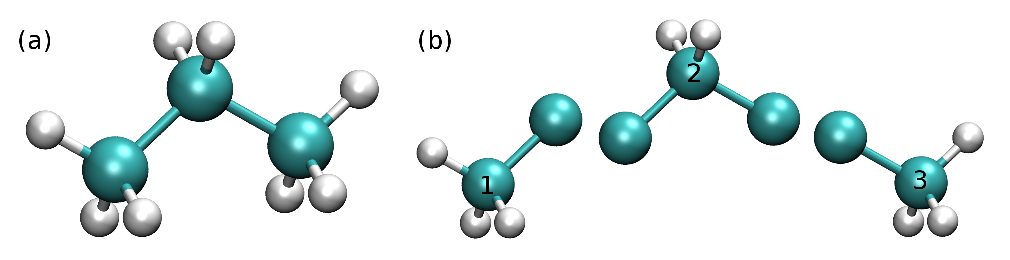
\includegraphics[width=0.99\textwidth]{c3.eps}
	\caption{(a) An all-atom model of propane. (b) The same model as in (a), but parsed into three fragments.}
	\label{fig:propaneFragments}
\end{figure}


\begin{enumerate}
  \item Select the order in which each fragment of the ($N+1$)th molecule will be placed. The probability of the resulting sequence is $p_{seq}$. (See example in Table. \ref{table:propane}.)
  \begin{enumerate}
		\item The first fragment $i$ is chosen with uniform probability 1/$N_{frag}$.
    \item Subsequent fragments must be connected to a previously chosen fragment and are chosen with the uniform probability 1/$N_{cnxn}$, where the number of connections $N_{cnxn}= \sum_{ij}{\delta_{ij} h_{i} (1-h_{j})}$ is summed over all fragments $i$ and $j$. $h_i$ is 1 if fragment $i$ has been previously chosen and 0 otherwise. $\delta_{ij}$ is 1 if fragments $i$ and $j$ are connected and 0 otherwise.
  \end{enumerate}
	\item Select a conformation for fragment $i$ with Boltzmann probability \newline $e^{-\beta U(\mathbf{q}_{frag_i})}d\mathbf{q}_{frag_i}/Z_{frag_i}$, where $\mathbf{q}_{frag_i}$ are the internal degrees of freedom (angles and/or impropers) associated with fragment $i$.
	\item Select an orientation with uniform probability $d\mathbf{q}_{rot}/Z_{rot}$. 
	\item Select a coordinate for the center of mass (COM) of fragment $i$:
	\begin{enumerate}
		\item Select $\kappa_{ins}$ trial coordinates $\mathbf{r}_k$, each with uniform probability $d\mathbf{r}/V$. Since one of the trial coordinates will be selected later, the individual probabilities are additive. The probability of the collection of trial coordinates is $\kappa_{ins}d\mathbf{r}/V$.
		\item Compute the change in potential energy $\Delta U_k^{ins}$ of inserting fragment $i$ at each position $\mathbf{r}_k$ into configuration $\mathbf{q}_m^N$.
		\item Select one of the trial coordinates with probability $e^{-\beta \Delta U_k^{ins}} / \sum_k{e^{-\beta \Delta U_k^{ins}}}$.
	\end{enumerate}
	\item For each additional fragment $j$:
	\begin{enumerate}
		\item Select a fragment conformation with Boltzmann probability\newline$e^{-\beta U(\mathbf{q}_{frag_j})}d\mathbf{q}_{frag_j}/Z_{frag_j}$
		\item Select the first of $\kappa_{dih}$ trial dihedrals $\phi_0$ with uniform probability from the interval [0,$\frac{2\pi}{\kappa_{dih}}$). Additional trial dihedrals are equally spaced around the unit circle, $\phi_k=\phi_{k-1}+2\pi/\kappa_{dih}$. The probability of selecting $\phi_0$ is $\kappa_{dih}d\phi/2\pi$.
		\item Compute the change in potential energy $\Delta U_k^{dih}$ of attaching fragment $j$ to the growing molecule with each dihedral $\phi_k$.
		\item Select one of the trial dihedrals with probability $e^{-\beta \Delta U_k^{dih}} / \sum_k{e^{-\beta \Delta U_k^{dih}}}$.
	\end{enumerate}
\end{enumerate}

\begin{table}
\caption{Possible sequences and probabilities for inserting the fragments of the all-atom model of propane shown in Fig. \ref{fig:propaneFragments}.}
\label{table:propane}
\centering
\begin{tabular}{|c|c|} \hline
 {\bf Sequence} & {\bf $p_{seq}$} \\ \hline
 1 2 3 & 1/3 \\
 2 1 3 & 1/6 \\
 2 3 1 & 1/6 \\
 3 2 1 & 1/3 \\
 \hline
\multicolumn{2}{c}{}
\end{tabular}
\end{table}

The overall probability $\alpha_{mn}$ of attempting the insertion with the selected position, orientation and conformation is 

\begin{align}
\alpha_{mn} &= p_{seq}\ \frac{d\mathbf{q}_{rot}}{Z_{rot}}\ \frac{\kappa_{ins}d\mathbf{r}}{V}\ \frac{e^{-\beta \Delta U_k^{ins}}}{\sum_k{e^{-\beta \Delta U_k^{ins}}}}\ \times \nonumber \\
&\ \ \ \left[\prod_{i=1}^{N_{frag}}{\frac{e^{-\beta U(\mathbf{q}_{frag_i})}d\mathbf{q}_{frag_i}}{Z_{frag_i}}}\right]\ \left[\prod_{j=1}^{N_{frag}-1}{\frac{\kappa_{dih}d\phi}{2\pi}\ \frac{e^{-\beta \Delta U_k^{dih}}}{\sum_k{e^{-\beta \Delta U_k^{dih}}}}}\right] \\
\label{eq:alpha_cbmcInsert}
&= p_{seq}\ p_{bias}\ \frac{e^{-\beta U(\mathbf{q}_{frag})}d\mathbf{q}}{VZ_{rot}Z_{frag}\Omega_{dih}}
\end{align}

where $Z_{frag} = \prod_i Z_{frag_i}$ is the configurational partition function over degrees of freedom internal to each fragment, $U(\mathbf{q}_{frag}) = \sum_iU(\mathbf{q}_{frag_i})$ is the summed potential energy of each of the (disconnected) fragments, $\Omega_{dih} = (2\pi)^{N_{frag}-1}$ and $p_{bias}$ is

\begin{equation}
p_{bias} = \frac{\kappa_{ins}\ e^{-\beta \Delta U_k^{ins}}}{\sum_k{e^{-\beta \Delta U_k^{ins}}}}\ \left[\prod_{j=1}^{N_{frag}-1}{\frac{\kappa_{dih}\ e^{-\beta \Delta U_k^{dih}}}{\sum_k{e^{-\beta \Delta U_k^{dih}}}}}\right]
\end{equation}

Note that the term $VZ_{rot}Z_{frag}\Omega_{dih}$ in the denominator of Eq.\ (\ref{eq:alpha_cbmcInsert}) differs from $Z(1,V,T)=VZ_{rot}Z_{int}$.

In the reverse move, 1 of the $N+1$ particles is randomly selected for deletion. The probability $\alpha_{nm}$ of picking the molecule we just inserted is

\begin{equation}
\label{eq:alpha_cbmcReverseInsert}
\alpha_{nm} = \frac{1}{N+1}
\end{equation}

Combining Eqs.\ (\ref{eq:alpha_cbmcInsert}) and (\ref{eq:alpha_cbmcReverseInsert}) with Eq.\ (\ref{eq:pMuVT_ratio}) or Eq.\ (\ref{eq:pfVT_ratio}) gives the acceptance probability for a CBMC insertion move

\begin{align}
\label{eq:pAcc_cbmcInsertMuShift}
\ln\left( \frac{\alpha_{mn}}{\alpha_{nm}} \frac{p_m}{p_n} \right) &= \beta \left[\Delta U - U(\mathbf{q}^{(N+1)}_{frag,n})\right] - \beta \mu' + \ln\left( \frac{(N+1)\Lambda^3}{V} \right) + \ln\left( p_{seq}p_{bias} \right) \\
\label{eq:pAcc_cbmcInsertFShift}
&= \beta \left[\Delta U - U(\mathbf{q}^{(N+1)}_{frag,n})\right] + \ln\left( \frac{N+1}{\beta f' V} \right) + \ln\left( p_{seq}p_{bias} \right)
\end{align}

where $\mu'$ and $f'$ are, respectively, a shifted chemical potential and a skewed fugacity,

\begin{align}
\label{eq:muShift}
\mu'&=\mu+k_BT\ln\left( Q_{rot+int} \frac{Z_{frag}\Omega_{dih}}{Z_{int}} \right) \\
\label{eq:fShift}
f'&= f \frac{Z_{frag}\Omega_{dih}}{Z_{int}}
\end{align}

All of the terms in Eqs.\ (\ref{eq:muShift}) and (\ref{eq:fShift}) are intensive. GCMC simulations using Eqs.\ (\ref{eq:pAcc_cbmcInsertMuShift}) and (\ref{eq:pAcc_cbmcInsertFShift}) will converge to the same average density regardless of the simulation volume $V$. However, the values of $\mu'$ or $f'$ that correspond to the converged density will {\em not} match tabulated values of $\mu$ or $f$ computed from experimental data.

Note that the term $Z^{IG}/\Omega$ from Macedonia {\em et al} \cite{Macedonia:1999}. would be equivalent to $Z_{int}/\Omega_{frag}\Omega_{dih}$ in the nomenclature used here. The configurational partition function of the disconnected fragments integrates over a Boltzmann factor, $Z_{frag} = \int e^{-\beta U(\mathbf{q}_{frag})} d\mathbf{q}_{frag}$, whereas the term $\Omega_{frag} = \int d\mathbf{q}_{frag}$ does not.

In Cassandra, the insertion move is implemented in the subroutine Insertion in insertion.f90. The relevant lines from version 1.1 are quoted below. The variable names in the insertion.f90 code are identified with symbols in Table \ref{table:cbmcInsert}.

\begin{minipage}{\linewidth}
\begin{lstlisting}[firstnumber=441, caption=insertion.f90]
  ln_pacc = beta(this_box) * (delta_e - E_angle - nrg_ring_frag_tot)
\end{lstlisting}
\begin{lstlisting}[firstnumber=447]
  ln_pacc = ln_pacc + DLOG(P_seq * P_bias) &
                    + DLOG(REAL(nmols(is,this_box)+1,DP)) &
                    - DLOG(box_list(this_box)%volume)

  IF(lchempot) THEN
     ! chemical potential is input
     ln_pacc = ln_pacc - species_list(is)%chem_potential * beta(this_box) &
               + 3.0_DP*DLOG(species_list(is)%de_broglie(this_box))
  ELSE   
     ! fugacity is input
     ln_pacc = ln_pacc - DLOG(species_list(is)%fugacity) &
                       - DLOG(beta(this_box)) &
  END IF 

  accept = accept_or_reject(ln_pacc)
\end{lstlisting}
\end{minipage}

Note that GCMC simulations using fugacities are currently not supported in Cassandra. This feature
will be implemented in a future release.

\begin{table}
\caption{Variable symbols and code names for inserting a molecule}
\label{table:cbmcInsert}
\centering
\begin{tabular}{|c|c|} \hline
 {\bf Symbol} & {\bf Code name} \\ \hline
 $\beta$ & beta(this\_box) \\
 $\Delta U$ & delta\_e \\
 $U(\mathbf{q}_{frag})$ & E\_angle + nrg\_ring\_frag\_tot \\
 $p_{seq}$ & P\_seq \\
 $p_{bias}$ & P\_bias \\
 $\mu'$ & species\_list(is)\%chem\_potential \\
 $N$ & nmols(is,this\_box) \\
 $V$ & box\_list(this\_box)\%volume \\
 $\Lambda$ & species\_list(is)\%de\_broglie(this\_box) \\
 $f'$ & species\_list(is)\%fugacity \\
 \hline
\multicolumn{2}{c}{}
\end{tabular}
\end{table}

\subsection{Deleting a Molecule that was Inserted via \newline Configurational Bias Monte Carlo}
\label{sec:cbmcDelete}

The probability $\alpha_{mn}$ of choosing a molecule to delete is

\begin{equation}
\alpha_{mn} = \frac{1}{N}
\end{equation}

The probability of the reverse move $\alpha_{nm}$ requires knowledge of the sequence and biasing probabilities $p_{seq}$ and $p_{bias}$ that would have been used to place the molecule if it was being inserted. $p_{seq}$ and $p_{bias}$ can be calculated using the following procedure:

\begin{enumerate}
  \item Select the fragment order using the same procedure for inserting a molecule. The probability of the resulting sequence is $p_{seq}$.
	\item The first fragment in the sequence is fragment $j$. Calculate the intramolecular potential energy of fragment $j$'s current conformation, $U(\mathbf{q}_{frag_j})$. The probability of this conformation is Boltzmann  $e^{-\beta U(\mathbf{q}_{frag_j})}d\mathbf{q}_{frag_j}/Z_{frag_j}$.
	\item The probability of the fragment's current orientation is $d\mathbf{q}_{rot}/Z_{rot}$. 
	\item Calculate the weight of the fragment's current center of mass (COM) coordinates:
	\begin{enumerate}
		\item Compute the interaction potential energy $\Delta U^{ins}$ between fragment $j$ and the other $N-1$ molecules.
		\item Select $\kappa_{ins}-1$ trial coordinates $\mathbf{r}_k$, each with uniform probability $d\mathbf{r}/V$.
		\item Calculate the weight of the fragment's current COM amongst the trial coordinates, $e^{-\beta \Delta U^{ins}} / \sum_k{e^{-\beta \Delta U_k^{ins}}}$.
	\end{enumerate}
	\item For each additional fragment $j$:
	\begin{enumerate}
		\item Calculate the intramolecular potential energy of fragment $j$'s current conformation, $U(\mathbf{q}_{frag_j})$. The weight of this conformation in the Boltzmann distribution is $e^{-\beta U(\mathbf{q}_{frag_j})}d\mathbf{q}_{frag_j}/Z_{frag_j}$.
		\item Calculate the interaction potential energy $\Delta U^{dih}$ between fragment $j$, on the one hand, and fragments $i$ through $j-1$ and the other $N-1$ molecules.
		\item Calculate the current dihedral $\phi_0$ of fragment $j$. Compute the interaction potential energy $\Delta U_k^{dih}$ at $\kappa_{dih}-1$ trial dihedrals $\phi_k = \phi_{k-1} + 2\pi/\kappa_{dih}$.
		\item Compute the weight of $\phi_0$ amongst the trial dihedrals, $e^{-\beta \Delta U^{dih}}/ \sum_k{e^{-\beta \Delta U_k^{dih}}}$.
	\end{enumerate}
\end{enumerate}

The overall probability $\alpha_{nm}$ is 

\begin{equation}
\label{eq:alpha_cbmcReverseDelete}
\alpha_{nm} = p_{seq}\ p_{bias}\ \frac{e^{-\beta U(\mathbf{q}_{frag})}d\mathbf{q}}{VZ_{rot}Z_{frag}\Omega_{dih}}.
\end{equation}

The acceptance criteria for deleting a molecule inserted via CBMC is

\begin{align}
\label{eq:pAcc_cbmcDeleteMuShift}
\ln\left( \frac{\alpha_{mn}}{\alpha_{nm}} \frac{p_m}{p_n} \right) &= \beta \left[\Delta U + U(\mathbf{q}^{(i)}_{frag,m})\right] + \beta \mu' + \ln\left( \frac{V}{N\Lambda^3} \right) - \ln\left( p_{seq}p_{bias} \right) \\
\label{eq_pAcc_cbmcDeleteF}
&= \beta \left[\Delta U + U(\mathbf{q}^{(i)}_{frag,m})\right] + \ln\left( \frac{\beta f' V}{N} \right) - \ln\left( p_{seq}p_{bias} \right)
\end{align}

In Cassandra, the deletion move is implemented in the subroutine Deletion in deletion.f90. The relevant lines are quoted below. The variable names in deletion.f90 code are identified with symbols in Table \ref{table:cbmcDelete}.

\begin{minipage}{\linewidth}
\begin{lstlisting}[firstnumber=334, caption=deletion.f90]
  ln_pacc = beta(this_box) * (delta_e + E_angle + nrg_ring_frag_tot)
\end{lstlisting}
\begin{lstlisting}[firstnumber=340]
  ln_pacc = ln_pacc - DLOG(P_seq * P_bias) &
                    - DLOG(REAL(nmols(is,this_box),DP)) &
                    + DLOG(box_list(this_box)%volume)
 
  IF(lchempot) THEN
     ! chemical potential is input
     ln_pacc = ln_pacc + beta(this_box) * species_list(is)%chem_potential &
             - 3.0_DP*DLOG(species_list(is)%de_broglie(this_box))
  ELSE
     ! fugacity is input
     ln_pacc = ln_pacc + DLOG(species_list(is)%fugacity) &
                       + DLOG(beta(this_box)) &
  END IF
 
  accept = accept_or_reject(ln_pacc)

\end{lstlisting}
\end{minipage}

Note that GCMC simulations using fugacities are currently not supported in Cassandra. This feature
will be implemented in a future release.

\begin{table}
\caption{Variable symbols and code names for deleting a molecule}
\label{table:cbmcDelete}
\centering
\begin{tabular}{|c|c|} \hline
 {\bf Symbol} & {\bf Code name} \\ \hline
 $\beta$ & beta(this\_box) \\
 $\Delta U$ & delta\_e \\
 $U(\mathbf{q}_{frag})$ & E\_angle + nrg\_ring\_frag\_tot \\
 $p_{seq}$ & P\_seq \\
 $p_{bias}$ & P\_bias \\
 $\mu'$ & species\_list(is)\%chem\_potential \\
 $N$ & nmols(is,this\_box) \\
 $V$ & box\_list(this\_box)\%volume \\
 $\Lambda$ & species\_list(is)\%de\_broglie(this\_box) \\
 $f'$ & species\_list(is)\%fugacity \\
 \hline
\multicolumn{2}{c}{}
\end{tabular}
\end{table}

\subsection{Regrowing a Molecule with Configurational Bias Monte Carlo}
\label{sec:cbmcRegrow}
Regrowing a molecule that has more than one fragment is a combination deletion and insertion move. Starting from microstate $m$:

\begin{enumerate}
	\item Randomly select a molecule with uniform probability $1/N$.
	\item Randomly select a bond to cut on the selected molecule with uniform probability $1/N_{bonds}$.
	\item Delete the fragments on one side of the bond or the other with equal probability. The number of deleted fragments is $N_{del}$.
	\item Reinsert the deleted fragments using the CBMC procedures for selecting the order of inserting the fragments, choosing a fragment conformation, and a connecting dihedral value (see Section \ref{sec:cbmcInsert}).
\end{enumerate}

The overall probability $\alpha_{mn}$ of attempting to regrow the molecule with the selected conformation is 

\begin{align}
\alpha_{mn} &= \frac{p_{seq}}{N N_{bonds}}\ \left[\prod_{j=1}^{N_{del}}{\frac{e^{-\beta U(\mathbf{q}^{(i)}_{frag_j})}d\mathbf{q}_{frag_j}}{Z_{frag_j}}}\right]\ \left[\prod_{j=1}^{N_{del}}{\frac{\kappa_{dih}d\phi}{2\pi}\ \frac{e^{-\beta \Delta U_k^{dih}}}{\sum_k{e^{-\beta \Delta U_k^{dih}}}}}\right] \nonumber \\
\label{eq:alpha_cbmcRegrow}
&= \frac{p_{seq}}{N N_{bonds}}\ \frac{e^{-\beta U(\mathbf{q}^{(i)}_{del,n})}d\mathbf{q}}{Z_{del}\Omega_{del}}\ p_{forward}
\end{align}

where $Z_{del} = \prod_i Z_{frag_j}$ is the configurational partition function over degrees of freedom internal to the deleted fragments, $U(\mathbf{q}^{(i)}_{del,n}) = \sum_jU(\mathbf{q}_{frag_j})$ is the summed potential energy of each deleted fragment with the conformations in microstate $n$, $\Omega_{del} = (2\pi)^{N_{del}}$ and $p_{forward}$ is the biasing probability

\begin{equation}
p_{forward} = \prod_{j=1}^{N_{del}}{\frac{\kappa_{dih}\ e^{-\beta \Delta U_k^{dih}}}{\sum_k{e^{-\beta \Delta U_k^{dih}}}}}
\end{equation}

The reverse move is identical except for the potential energy of the deleted fragments $U(\mathbf{q}^{(i)}_{del,m})$ in microstate $m$ and the biasing probability $p_{reverse}$ which will depend on the values of the connecting dihedrals. Using Eqs. (\ref{eq:pNVT_ratio}) and (\ref{eq:alpha_cbmcRegrow}), the acceptance criteria is:

\begin{equation}
\label{eq:pAcc_cbmcRegrow}
\ln\left( \frac{\alpha_{mn}}{\alpha_{nm}} \frac{p_m}{p_n} \right) = \beta \left[\left( U(\mathbf{q}^N_n) - U(\mathbf{q}^{(i)}_{del,n})\right) - \left(U(\mathbf{q}^N_m) - U(\mathbf{q}^{(i)}_{del,m})\right)\right] + \ln\left( \frac{p_{forward}}{p_{reverse}} \right)
\end{equation}

Eq. (\ref{eq:pAcc_cbmcRegrow}) is implemented in subroutine cut\_N\_grow() in file cutNgrow.f90. 

\begin{minipage}{\linewidth}
\begin{lstlisting}[firstnumber=392, caption=cutNgrow.f90, label=code:cbmcRegrow]
  ln_pacc = beta(this_box) * (delta_e_n - nrg_ring_frag_forward) &
          - beta(this_box) * (delta_e_o - nrg_ring_frag_reverse) &
          + DLOG(P_forward / P_reverse)

  accept = accept_or_reject(ln_pacc)
\end{lstlisting}
\end{minipage}

\begin{table}
\caption{Variable symbols and code names for regrowing a molecule}
\label{table:cbmcRegrow}
\centering
\begin{tabular}{|c|c|} \hline
 {\bf Symbol} & {\bf Code name} \\ \hline
 $\beta$ & beta(this\_box) \\
 $U(\mathbf{q}^N_n) - U(\mathbf{q}^{(i)}_{del,n})$ & delta\_e\_n - nrg\_ring\_frag\_forward \\
 $U(\mathbf{q}^N_m) - U(\mathbf{q}^{(i)}_{del,m})$ & delta\_e\_o - nrg\_ring\_frag\_reverse \\
 $p_{forward}$ & P\_forward \\
 $p_{reverse}$ & P\_reverse \\
 \hline
\multicolumn{2}{c}{}
\end{tabular}
\end{table}

\section{Gibbs Ensemble Monte Carlo} 
\label{sec:gibbs}

The Gibbs Ensemble Monte Carlo method is a standard technique for studying phase equilibria of pure fluids
and mixtures. It is oftentimes the method of choice to study vapor-liquid equilibria due to its intuitive 
physical basis. 
In Cassandra, the NVT and NPT versions of the Gibbs Ensemble (GEMC-NVT and GEMC-NPT) are implemented. 
The GEMC-NVT method is suitable for simulating vapor liquid equilibria of pure systems, since
pure substances require the specification of only one intensive variable 
(temperature) to completely specify a state of two phases. 
By contrast, mixtures require the specification of an additional degree of freedom (pressure).
Thus, in the GEMC-NPT method, the pressure is specified in addition to temperature. \\

In section \ref{sec:gibbs_nvt}, the acceptance rules for the NVT version will be derived and 
references to their implementation in Cassandra will be
presented. For information about the implementation of the NPT version, 
please refer to section \ref{sec:gibbs_npt}

\subsection{Gibbs Ensemble-NVT}
\label{sec:gibbs_nvt}

In the GEMC-NVT method, the system is comprised by two boxes, one representing a vapor phase 
(denoted by superscript \textit{v}) and the other representing a liquid phase (denoted by superscript \textit{l}).
These boxes are in thermal contact with a heat bath that maintains them at constant temperature, thus ensuring
thermal equilibrium.
To achieve phase equilibrium, the boxes are allowed to exchange volume and particles under the constraint of constant total volume ($V^t=V^l + V^v$)
and constant number of particles ($N^t=N^l + N^v$). The partition function of this system is

\begin{equation}
Q\left(N^t,V^t,T\right) = \frac{1}{\Lambda^{3N^t}N^t!} \sum^{N^t}_{N{^l}} \frac{N^t!}{N^l!N^v!} \int^{V^t}_0  dV^l (V^l)^{N^l} (V^v)^{N^v} \int d \textbf{s}^{N^l} e^{-\beta U\left(\textbf{s}^{N^l}\right)} \int d \textbf{s}^{N^v} e^{-\beta U\left(\textbf{s}^{N^v}\right)}
\label{eq:gemc_nvt_partition}
\end{equation}


Where $\Lambda$ is the de Broglie wavelength, $\textbf{s}^{N^l}$ and $\textbf{s}^{N^v}$ are the scaled coordinates of the atoms in the two phases, $U\left(\textbf{s}^{N^l}\right)$ and $U\left(\textbf{s}^{N^v}\right)$ are the potential energies of the liquid and the vapor box, respectively. The microstate probability distribution is

\begin{equation}
p_m \propto (V^l)^{N^l} (V^v)^{N^v} e^{-\beta U \left(\textbf{s}^{N^l}\right) -\beta U \left(\textbf{s}^{N^v}\right)}
\label{eq:gemc_nvt_prob_dist}
\end{equation}

Note that the particle number factorials are not included in equation \ref{eq:gemc_nvt_prob_dist}, as particles are
distinguishable in a simulation (see also equation \ref{eq:pMuVT}). \\

In the GEMC-NVT technique, thermal equilibrium is attained by performing translation, rotation and regrowth moves. 
The acceptance rules for these moves can be extracted from the probability 
distribution \ref{eq:gemc_nvt_prob_dist}, and their functional form is exactly the same as that presented
in sections \ref{sec:translate}, \ref{sec:rotate}, \ref{sec:regrow} and \ref{sec:cbmcRegrow}, namely \\


\begin{equation}
\ln \left( \frac{\alpha_{mn}}{\alpha_{nm}} \frac{p_m}{p_n} \right) = - \beta \Delta U
\end{equation}


Exchange of volume between the two boxes is carried out to achieve pressure equilibrium. Assuming 
volume is being transfered from box A to box B, the 
acceptance rule is also derived from equation \ref{eq:gemc_nvt_prob_dist} and yields

\begin{equation}
\ln \left( \frac{\alpha_{mn}}{\alpha_{nm}} \frac{p_m}{p_n} \right) = - \beta \Delta U^A - \beta \Delta U^B + N^A \ln\left(\frac{V^A_m}{V^A_n}\right) + N^B \ln\left(\frac{V^B_m}{V^B_n}\right)
\label{eq:gemc_nvt_volume}
\end{equation}

\begin{table}
\caption{Variable symbols and code names for the volume scaling move in the GEMC-NVT method.}
\label{table:gemc_nvt_volume}
\centering
\begin{tabular}{|c|c|} \hline
 {\bf Symbol} & {\bf Code name} \\ \hline
 $\beta^A$ & beta(box1) \\
 $\beta^B$ & beta(box2) \\
 $\Delta U^A$ & delta\_e\_1 \\
 $\Delta U^B$ & delta\_e\_2 \\
 $N^A$ & tot\_mol\_box\_1 \\
 $N^B$ & tot\_mol\_box\_2 \\
 $V^A_m$ & box\_list(box1)\%volume \\
 $V^B_m$ & box\_list(box2)\%volume \\
 $V^A_n$ & box\_list\_old\_1\%volume \\
 $V^B_n$ & box\_list\_old\_2\%volume \\
 \hline
\multicolumn{2}{c}{}
\end{tabular}
\end{table}



This acceptance rule is implemented in the file gemc\_nvt\_volume.f90 as follows

\begin{minipage}{\linewidth}
\begin{lstlisting}[firstnumber=475, caption=gemc\_nvt\_volume.f90]
factor = beta(box1) * delta_e_1 + beta(box2) * delta_e_2 - &
                 tot_mol_box1 * DLOG( box_list(box1)%volume / box_list_old_1%volume) - &
                 tot_mol_box2 * DLOG( box_list(box2)%volume / box_list_old_2%volume)

\end{lstlisting}
\end{minipage}

Finally, exchange of particles is conducted between the two boxes to attain equality of chemical potentials.
If the particle is transfered from box A into box B, the acceptance rule for this move is

\begin{equation}
\ln \left( \frac{\alpha_{mn}}{\alpha_{nm}} \frac{p_m}{p_n} \right) = \ln \left( \frac{\alpha_{mn}}{\alpha_{nm}} \right)  \ln \left(\frac{V^B}{V^A}\right) -\beta \Delta U^A - \beta \Delta U^B
\label{eq:gemc_nvt_transfer}
\end{equation}

Note that in contrast to the volume move, the particle swap is not a symmetric move, as it might 
involve configurational biased regrowths. For the case of transfering a molecule from box A into box B, the forward probability $\alpha_{nm}$ is calculated
as follows

\begin{enumerate}
\item Pick box A
\item Pick a molecule from box A out of the $N^A_n$ possible molecules
\item Insert molecule in box B using protocol presented in section \ref{sec:cbmcInsert}
\end{enumerate}

The attempt probability of generating configuration m is

\begin{align}
\alpha_{nm} &= \frac{1}{2} \frac{1}{N^A_n} p_{seq_{nm}}\ \frac{d\mathbf{q}_{rot}}{Z_{rot}}\ \frac{\kappa_{ins}V^B d\mathbf{s}}{V^B}\ \left[\frac{e^{-\beta \Delta U_k^{ins}}}{\sum_k{e^{-\beta \Delta U_k^{ins}}}}\right]^B\ \times \nonumber \\
&\ \ \ \left[\prod_{i=1}^{N_{frag}}{\frac{e^{-\beta U(\mathbf{q}_{frag_i})}d\mathbf{q}_{frag_i}}{Z_{frag_i}}}\right]_{nm}\ \left[\prod_{j=1}^{N_{frag}-1}{\frac{\kappa_{dih}d\phi}{2\pi}\ \frac{e^{-\beta \Delta U_k^{dih}}}{\sum_k{e^{-\beta \Delta U_k^{dih}}}}}\right]_{nm} \\
\label{eq:gemc_nvt_transfer_forward}
& = \frac{1}{2} \frac{1}{N^A_n} p_{seq_{nm}}\ p_{bias_{nm}}\ \frac{e^{-\beta U(\mathbf{q}_{frag_{nm}})}d\mathbf{q}_{rot}d\mathbf{s}\prod_{i=1}^{N_{frag}}d\mathbf{q}_{frag_{i,nm}}\prod_{j=1}^{N_{frag}-1}d\phi_{nm}}{Z_{rot}Z_{frag}\Omega_{dih}}
\end{align}


Once the new configuration $m$ has been generated, the reverse probability $\alpha_{mn}$ must be calculated. This represents
the probability of generating the old state n, pretending that the current state is m.
The procedure is similar as before

\begin{enumerate}
\item Pick box B
\item Pick the swapped molecule from box B of the $N^B_n+1$ possible molecules
\item Insert molecule back in box A using protocol presented in section \ref{sec:cbmcInsert}
\end{enumerate}

The attempt probability of generating the old configuration n pretending we are in the new configuration m is

\begin{equation}
\alpha_{mn} = \frac{1}{2} \frac{1}{N^B_n+1} p_{seq_{mn}}\ p_{bias_{mn}}\ \frac{e^{-\beta U(\mathbf{q}_{frag_{mn}})}d\mathbf{q}_{rot}d\mathbf{s}\prod_{i=1}^{N_{frag}}d\mathbf{q}_{frag_{i,mn}}\prod_{j=1}^{N_{frag}-1}d\phi_{mn}}{Z_{rot}Z_{frag}\Omega_{dih}}
\label{eq:gemc_nvt_transfer_reverse}
\end{equation}

The acceptance rule now becomes
\begin{equation}
\ln \left( \frac{\alpha_{mn}}{\alpha_{nm}} \frac{p_m}{p_n} \right) = \ln \left( \frac{ p_{bias_{mn}}}{p_{bias_{nm}}} \frac{N^A_n}{N^B_n+1} \frac{V^B}{V^A} \right) + \beta U(\mathbf{q}_{frag_{nm}})- \beta U(\mathbf{q}_{frag_{mn}}) -\beta \Delta U^A - \beta \Delta U^B
\label{eq:gemc_transfer_final}
\end{equation}

Note that the terms $p_{seq}$ cancelled out, as the same fragment regrowth sequence is used in the forward and reverse moves.
The implementation of the particle swap move is found in the file gemc\_particle\_transfer.f90 as follows

\begin{table}
\caption{Variable symbols and code names for the particle transfer move in the GEMC-NVT method.}
\label{table:gemc_transfer}
\centering
\begin{tabular}{|c|c|} \hline
 {\bf Symbol} & {\bf Code name} \\ \hline
 $\beta^A$ & beta(box\_out) \\
 $\beta^B$ & beta(box\_in) \\
 $\Delta U^A$ & -delta\_e\_out \\
 $\Delta U^B$ & delta\_e\_in \\
 $U(\mathbf{q}_{frag_{nm}})$ & e\_angle\_in + nrg\_ring\_frag\_in \\
 $U(\mathbf{q}_{frag_{mn}})$ & e\_angle\_out + nrg\_ring\_frag\_out \\
 $V^A_m$ & box\_list(box\_out)\%volume \\
 $V^B_m$ & box\_list(box\_in)\%volume \\
 $p_{bias_{nm}}$ & P\_forward \\
 $p_{bias_{mn}}$ & P\_reverse \\
 \hline
\multicolumn{2}{c}{}
\end{tabular}
\end{table}

\begin{minipage}{\linewidth}
\begin{lstlisting}[firstnumber=505, caption=gemc\_particle\_transfer.f90]
delta_e_in_pacc = delta_e_in
delta_e_out_pacc = delta_e_out
\end{lstlisting}

\begin{lstlisting}[firstnumber=518]
delta_e_in_pacc = delta_e_in_pacc - e_angle_in - nrg_ring_frag_in
delta_e_out_pacc = delta_e_out_pacc - e_angle_out - nrg_ring_frag_out
\end{lstlisting}


\begin{lstlisting}[firstnumber=526]
ln_pacc = beta(box_in)*delta_e_in_pacc - beta(box_out)*delta_e_out_pacc

ln_pacc = ln_pacc - DLOG(box_list(box_in)%volume) &
                    + DLOG(box_list(box_out)%volume) &
                    - DLOG(REAL(nmols(this_species,box_out),DP)) &
                    + DLOG(REAL(nmols(this_species,box_in) + 1, DP))

ln_pacc = ln_pacc + DLOG(P_forward / P_reverse)
accept = accept_or_reject(ln_pacc)
\end{lstlisting}
\end{minipage}


\subsection{Gibbs Ensemble-NPT} 
\label{sec:gibbs_npt}

In the GEMC-NPT method, the system is comprised of two boxes. These boxes are allowed to exchange
particles to attain equality of chemical potential. In contrast to
the GEMC-NVT method, the volume of each box is allowed to fluctuate
independently from the other box. As a result, the total volume of the system is not constant and the 
pressure must be specified as a simulation parameter in addition to the temperature.
This is consistent with the Gibbs phase rule for mixtures, which requires the specification of two intensive
variables (e.g. pressure and temperature) to fully specify a state with two phases. \\

The probability distribution of this ensemble is very similar to its NVT counterpart (see
equation \ref{eq:gemc_nvt_prob_dist}), 

\begin{equation}
p_m \propto (V^l)^{N^l} (V^v)^{N^v} e^{-\beta U \left(\textbf{s}^{N^l}\right) -\beta U \left(\textbf{s}^{N^v}\right)
- \beta P \left(V^l + V^v\right) }
\label{eq:gemc_npt_prob_dist}
\end{equation}

Thermal equilibration moves can be derived from the above probability distribution. They involve
the usual translation, rotation and regrowth moves. The functional form of the acceptance rule
is the same as those exposed in 
sections \ref{sec:translate}, \ref{sec:rotate}, \ref{sec:regrow}, \ref{sec:cbmcRegrow}.
Similarly, particle swap moves are carried out in the same way as it was exposed in section \ref{sec:gibbs_nvt}. 
Finally, volume moves are carried out by picking one of the boxes and performing a volume change using the protocol
exposed in section \ref{subsec:scaling_the_volume}. 





\section{Multicomponent Systems} 

Excluding section \ref{sec:gibbs_npt}, the acceptance rules for all the Monte Carlo techniques exposed in this chapter
have been developed for pure component systems. The Monte Carlo moves and acceptance criteria for multicomponent systems are straightforward extensions of the pure component moves. The only modification needed to translate, rotate and regrow molecules is to first select a species. In these moves, a species is selected randomly in proportion to its mole fraction $N_i/N$. When inserting and deleting a molecule, the mole fractions of each species change. In these cases, a species in a multicomponent system is selected instead with uniform probability $1/N_{species}$. In either case, species selection is symmetric for both forward and reverse moves and so cancels from the acceptance criterion.

%In contrast, a reaction move that changes the number of molecules of several species simultaneously will depend on the chemical potentials of each species. In the multicomponent grand canonical ensemble, the temperature $T$, volume $V$ and set of chemical potentials $\{\mu\} = \mu_1, \ldots, \mu_s$ of each species are held constant. The partition function for a system with $s$ species is
%
%\begin{equation}
%\label{eq:partitionFn_MuiVT}
%\Xi(\{\mu\},V,T) = \sum\limits_{N_1=0}^{\infty} \ldots \sum\limits_{N_s=0}^{\infty}Q(\{N\},V,T)\ e^{\beta \mu_i N_i}
%\end{equation}
%
%where $\{N\}$ is the set of $s$ molecule numbers, and a summation is implied over the term $\mu_i N_i$. The probability of the system having $\{N\}$ molecules is 
%
%\begin{equation}
%\label{eq:pNi}
%p(\{N\}) = \frac{Q(\{N\},V,T)e^{\beta \mu_i N_i}}{\Xi(\{\mu\},V,T)}
%\end{equation}
%
%The probability of observing microstate $m$ with $\{N\}_m$ molecules and configuration $\{\mathbf{q}^N\}_m$ is
%
%\begin{align}
%\label{eq:pMuiVT}
%p_m &= \frac{e^{-\beta U_m} \prod\limits_{i=1}^s{d\mathbf{q}_i^{N_{im}}}}{Z(\{N\}_m,V,T)}\ \frac{Q(\{N\}_m,V,T)e^{\beta \mu_i N_{im}}}{\Xi(\{\mu\},V,T)} \nonumber \\
%&= \frac{e^{-\beta U_m + \beta \mu_i N_{im}}}{\Xi(\{\mu\},V,T)}\ \prod\limits_{i=1}^s\left[\frac{Q_i(1,V,T)}{Z_i(1,V,T)}\ d\mathbf{q}_i\right]^{N_{im}}
%\end{align}
%
%The ratio of microstate probabilities is
%
%\begin{equation}
%\label{eq:pMuiVT_ratio}
%\frac{p_m}{p_n} = e^{\beta \Delta U - \beta \mu_i \Delta N_i}\ \prod\limits_{i=1}^s\left[\frac{Q_i(1,V,T)}{Z_i(1,V,T)}\ d\mathbf{q}_i\right]^{-\Delta N_i}
%\end{equation}
%
%\subsection{Reaction Ensemble Monte Carlo (RxMC)}
%\label{sec:rxmc}
%In Reaction Ensemble Monte Carlo, the number of molecules of each species can only change by a stoichiometric amount $\nu_i$ as a reaction occurs. For reactants $\nu_i<0$; for products $\nu_i>0$. Reaction equilibrium occurs when the following condition is met
%
%\begin{equation}
%\label{eq:rxnEquil}
%\sum\limits_{i=1}^{s}{\nu_i \mu_i} = 0
%\end{equation}
%
%\noindent
%Substituting Eq. (\ref{eq:rxnEquil}) and $\Delta N_i = \nu_i$ into Eq. (\ref{eq:pMuiVT_ratio}) gives
%
%\begin{equation}
%\label{eq:pMuiVT_ratio_2}
%\frac{p_m}{p_n} = e^{\beta \Delta U}\ \prod\limits_{i=1}^s\left[\frac{Q_i(1,V,T)}{Z_i(1,V,T)}\ d\mathbf{q}_i\right]^{-\nu_i}
%\end{equation}
%
%\noindent
%The product of partition functions can be replaced by the equilibrium constant of an ideal gas $K_{eq}$ or the standard change in free energy of the reaction $\Delta G_{rxn}^{o}$ at standard pressure $P\degree$
%
%\begin{equation}
%\label{eq:Keq_ideal}
%\prod\limits_{i=1}^s{\left(\frac{Q_i(1,V,T)}{V}\right)^{\nu_i}} = K_{eq} = e^{-\beta \Delta G_{rxn}^{o}} \left(\frac{P\degree}{k_BT}\right)^{\Delta \nu}
%\end{equation}
%
%\noindent
%where $\Delta \nu = \sum_i \nu_i$ and $K_{eq}$ has units $[\textrm{volume}]^{-\Delta \nu}$. Substituting Eq. (\ref{eq:Keq_ideal}) and $Z_i(1,V,T) = VZ_{rot,i}Z_{int,i}$ into Eq. (\ref{eq:pMuiVT_ratio_2}) gives
%
%\begin{align}
%\label{eq:pMuiVT_ratio_3}
%\frac{p_m}{p_n} &= e^{\beta \Delta U}\ K_{eq}^{-1}\ \prod\limits_{i=1}^s\left[\frac{d\mathbf{q}_i}{Z_{rot,i}Z_{int,i}}\right]^{-\nu_i} \\
%\label{eq:pMuiVT_ratio_4}
%&= e^{\beta \Delta U + \beta \Delta G_{rxn}^{o}}\ \prod\limits_{i=1}^s\left[\frac{P\degree d\mathbf{q}_i}{k_BT\ Z_{rot,i}Z_{int,i}}\right]^{-\nu_i}
%\end{align}
%
%\noindent
%In the liquid phase, the change in energy $\Delta U$ from deleting reactants and inserting products in one step is prohibitively high. And yet, the number of molecules of each species $i$ must change by $\nu_i$ in a single step for Eqs. (\ref{eq:pMuiVT_ratio_3}-\ref{eq:pMuiVT_ratio_4}) to apply. 
%
%In Cassandra, reactants are phased out of the system as products are phased in using multiple steps. For example, to simulate the reaction
%
%\begin{equation}
%\label{eq:rxnABC}
%A + B \rightleftharpoons C
%\end{equation}
%
%\noindent
%an ideal gas (i.e., non-interacting) molecule of $C$, $C_0$, is inserted into the simulation box. Then the interaction of $C_0$ is increased as the interaction of $A$ and $B$ is decreased
%
%\begin{equation}
%\label{eq:rxnABC_lambda}
%A + B + C_0 \rightleftharpoons A_{1-x} + B_{1-x} + C_x \rightleftharpoons A_0 + B_0 + C
%\end{equation}
%
%\noindent
%where $x$ is the extent of the reaction and the subscripts indicate how strongly a molecule interacts with other molecules in the system. The initial state $A + B + C_0$ corresponds to $x=0$; there is one molecule $C_0$ that does not interact with any other molecules, whereas all $A$ and $B$ molecules interact fully with the rest of the system. The final state $A_0 + B_0 + C$ corresponds to $x=1$; there is one molecule each $A_0$ and $B_0$ that do not interact  with any other molecules, whereas all $C$ molecules interact fully with the rest of the system. At intermediate states $A_{1-x} + B_{1-x} + C_x$, $x$ can take on fixed values between 0 and 1 (e.g. 0.2, 0.4, 0.6, 0.8). The molecules involved in the reaction have been tagged; in this example, there is one fractional molecule of each species. In each case, the number of molecules of all species is constant. At either end point (x=0 or x=1), the ideal gas molecules can react according to 
%
%\begin{equation}
%\label{eq:rxnABC_ideal}
%A_0 + B_0 \rightleftharpoons C_0
%\end{equation}
%
%\noindent
%where, in the forward direction, the ideal gas reactants are deleted from the system and ideal gas products are inserted. The number of molecules of each species changes by $\nu_i$. 
%
%Reaction equilibrium is established by changing the extent of reaction using a series of moves:
%
%\begin{itemize}
%	\item Increment from $x_1=0$ to $x_2>0$.
%	\item Increment from $x_1$ to $x_2$, where $0 < x_1 < x_2 < 1$.
%	\item Increment from $x_1<1$ to $x_2=1$.
%	\item React in the ideal gas phase: change from $x_1=1$ to $x_2=0$.
%\end{itemize}
%
%\noindent
%Each move can occur in the forward and reverse direction. Acceptance criteria are derived for each forward move.
%
%\subsection{Increment from $x_1=0$ to $0<x_2<1$}
%The number of molecules in the system does not change, so Eq. (\ref{eq:pMuiVT_ratio}) reduces to 
%
%\begin{equation}
%\label{eq:pMuiVT_noDeltaN}
%\frac{p_m}{p_n} = e^{\beta \Delta U}
%\end{equation}
%
%\noindent
%The probability of generating microstate $n$ from microstate $m$ is the probability of selecting $-\nu_i$ reactant molecules of each species from the $N_{im}$ integer molecules in the system
%
%\begin{equation}
%\alpha_{mn} = \prod_{i \in react} \frac{(-\nu_i)!(N_{im}+\nu_i)!}{N_{im}!}
%\end{equation}
%
%\noindent
%In the reverse step, no molecules need to be chosen. The probability $\alpha_{nm}=1$. The acceptance criteria is therefore
%
%\begin{equation}
%\ln\left( \frac{\alpha_{mn}}{\alpha_{nm}} \frac{p_m}{p_n} \right) = \beta \Delta U  + \ln\left( \prod_{i \in react}\frac{(-\nu_i)!(N_{im}+\nu_i)!}{N_{im}!} \right)
%\end{equation}
%
%\noindent
%If there is not a stoichiometric amount of any reactant in microstate $m$, this move will not be attempted.
%
%\subsection{Increment from $x_1$ to $x_2$, where $0<x_1<x_2<1$}
%The ratio of microstate probabilities is given by Eq. (\ref{eq:pMuiVT_noDeltaN}). No molecules need to be selected in either the forward or reverse direction, so $\alpha_{mn}=\alpha_{nm}=1$. The acceptance criteria is
%
%\begin{equation}
%\ln\left( \frac{\alpha_{mn}}{\alpha_{nm}} \frac{p_m}{p_n} \right) = \beta \Delta U
%\end{equation}
%
%\subsection{Increment from $x_1<1$ to $x_2=1$}
%The ratio of microstate probabilities is given by Eq. (\ref{eq:pMuiVT_noDeltaN}). No molecules need to be selected in the forward direction, so $\alpha_{nm}=1$. In the reverse step, the probability of generating microstate $m$ from microstate $n$ is the probability of selecting $\nu_i$ product molecules of each species from the $N_{in}=N_{im}+\nu_i$ integer molecules in the system
%
%\begin{equation}
%\alpha_{nm} = \prod_{i \in prod} \frac{\nu_i!N_{im}!}{(N_{im}+\nu_i)!}
%\end{equation}
%
%\noindent
%The acceptance criteria is 
%
%\begin{equation}
%\ln\left( \frac{\alpha_{mn}}{\alpha_{nm}} \frac{p_m}{p_n} \right) = \beta \Delta U  + \ln\left( \prod_{i \in prod}\frac{(N_{im}+\nu_i)!}{\nu_i!N_{im}!} \right)
%\end{equation}
%
%\subsection{React in the ideal gas phase: change from $x_1=1$ to $x_2=0$}
%In this step, the number of molecules of each species $i$ changes by $\nu_i$. The ratio of microstate probabilities is given by Eqs. (\ref{eq:pMuiVT_ratio_3}-\ref{eq:pMuiVT_ratio_4}). In the forward move, the ideal gas reactants are deleted and ideal gas products are inserted. The probability of generating microstate $n$ from microstate $m$ is the probability of inserting the ideal gas products (see Eq. (\ref{eq:alpha_randomInsert}) and the discussion that proceeds it) 
%
%\begin{equation}
%\alpha_{mn} = \prod_{i \in prod} \frac{e^{-\beta U_{int,i}}d\mathbf{q}_i}{Z_i(1,V,T)}
%\end{equation}
%
%\noindent
%where $U_{int,i}$ is the internal energy of the inserted molecule. In the reverse move, ideal gas reactants are inserted with probability
%
%\begin{equation}
%\alpha_{nm} = \prod_{i \in react} \frac{e^{-\beta U_{int,i}}d\mathbf{q}_i}{Z_i(1,V,T)}
%\end{equation}
%
%\noindent
%The ratio of the forward and reverse move is
%
%\begin{equation}
%\frac{\alpha_{mn}}{\alpha_{nm}} = \exp \left(-\beta \sum_{i \in prod} U_{int,i} + \beta \sum_{i \in react} U_{int,i} \right) \prod_{i=1}^s \left( \frac{d\mathbf{q}_i}{Z_i(1,V,T)} \right)^{\nu_i}
%\end{equation}
%
%\noindent
%where the sums are over the ideal gas molecules and the product is over the species. Since the molecules being inserted and deleted do not interact with any other molecules, the change in energy between microstates $m$ and $n$ is only due to the internal energy of the ideal gas molecules
%
%\begin{equation}
%\Delta U = \sum_{i \in prod} U_{int,i} - \sum_{i \in react} U_{int,i}
%\end{equation}
%
%\noindent
%The change in energy cancels from the acceptance criteria
%
%\begin{align}
%\ln\left( \frac{\alpha_{mn}}{\alpha_{nm}} \frac{p_m}{p_n} \right) &= \beta \Delta G_{rxn}^{o} + \ln \left( \prod_{i=1}^s \left[ \frac{P\degree d\mathbf{q}_i}{k_BT Z_{rot,i}Z_{int,i}} \frac{Z_i(1,V,T)}{d\mathbf{q}_i} \right]^{-\nu_i} \right) \\
%&= \beta \Delta G_{rxn}^{o} - \Delta \nu \ln(\beta P^o V)
%\end{align}
%
%\noindent
%Since the acceptance criteria does not depend on the configuration of molecules, the move can be accepted or rejected before generating microstate $n$.

\section{Appendix}
\label{sec:appendix}
\subsection{Inserting a Molecule Randomly}
\label{sec:randomInsert}
To insert a molecule, a position, orientation and molecular conformation must each be selected. The probability of inserting the new molecule at a random location is $d\mathbf{r}/V$, where $d\mathbf{r}$ is a Cartesian volume element of a single atom. The probability of choosing the molecule orientation is $d\mathbf{q}_{rot}/Z_{rot}$, which for a linear molecule is $d \cos(\theta) d\phi / 4\pi$ and for a nonlinear molecule is $d \cos(\theta)d\phi d\psi/8\pi^2$. The probability of the molecule conformation only depends on the remaining $2M-5$ internal bond angles, dihedral angles and improper angles $\mathbf{q}_{int}$. A thermal ensemble of configurations is Boltzmann distributed $e^{-\beta U(\mathbf{q}_{int})}/Z_{int}$. The overall probability $\alpha_{mn}$ is

\begin{equation}
\label{eq:alpha_randomInsert}
\alpha_{mn} = \frac{d\mathbf{r}}{V}\ \frac{d\mathbf{q}_{rot}}{Z_{rot}}\ \frac{e^{-\beta U(\mathbf{q}_{int,N+1,n})}}{Z_{int}}\ d\mathbf{q}_{int} = \frac{e^{-\beta U(\mathbf{q_{N+1,n}})}}{Z(1,V,T)}\ d\mathbf{q}.
\end{equation}

\noindent
where we have used Eq.\ (\ref{eq:configPartitionFn_1VT}) to recover $Z(1,V,T)$ and recognized that only internal degrees of freedom contribute to the potential energy of the isolated $N+1$th molecule in microstate $n$, $U(\mathbf{q}_{N+1,n}) = U(\mathbf{q}_{int,N+1,n})$. For a point particle with no rotational or internal degrees of freedom, $\alpha_{mn}$ reduces to $d\mathbf{r}/V$. For molecules with internal flexibility, a library of configurations distributed according to $e^{-\beta U(\mathbf{q}_{int})}/Z_{int}$ can be generated from a single molecule MC simulation. In the reverse move, 1 of the $N+1$ particles is randomly selected for deletion. The probability $\alpha_{nm}$ of picking the molecule we just inserted is

\begin{equation}
\alpha_{nm} = \frac{1}{N+1}
\end{equation}

\noindent
The acceptance probability for a random insertion move is 

\begin{equation}
\label{eq:pAcc_randomInsertMu}
\ln\left( \frac{\alpha_{mn}}{\alpha_{nm}} \frac{p_m}{p_n} \right) = \beta \left[\Delta U - U(\mathbf{q}_{N+1})\right] - \beta \mu + \ln\left( \frac{N+1}{Q(1,V,T)} \right)
\end{equation}

\noindent
where $U(\mathbf{q}_{N+1})$ is the intramolecular potential energy of the inserted molecule. $Q(1,V,T)$ is typically not known {\em a priori}, nor is it easily estimated. Substituting Eq.\ (\ref{eq:partitionFn_1VT}) into Eq.\ (\ref{eq:pAcc_randomInsertMu}) and absorbing $Q_{rot+int}$ into a shifted chemical potential $\mu'$

\begin{equation}
\mu' = \mu - k_BT\ln(Q_{rot+int})
\end{equation}

\noindent
gives the acceptance criteria for inserting a molecule

\begin{equation}
\label{eq:pAcc_randomInsertMuShift}
\ln\left( \frac{\alpha_{mn}}{\alpha_{nm}} \frac{p_m}{p_n} \right) = \beta \left[\Delta U - U(\mathbf{q}_{N+1})\right] - \beta \mu' + \ln\left( \frac{(N+1)\Lambda^3}{V} \right).
\end{equation}

\noindent
The terms absorbed into $\mu'$ are intensive and therefore GCMC simulations using Eq.\ (\ref{eq:pAcc_randomInsertMuShift}) will converge to a specific average density. However, the value of $\mu'$ that corresponds to the converged density will {\em not} match tabulated values of $\mu$ computed from experimental data.

Substituting Eq.\ (\ref{eq:mu}) into Eq.\ (\ref{eq:pAcc_randomInsertMu}) gives

\begin{equation}
\label{eq:pAcc_randomInsertF}
\ln\left( \frac{\alpha_{mn}}{\alpha_{nm}} \frac{p_m}{p_n} \right) = \beta \left[\Delta U - U(\mathbf{q}_{N+1})\right] + \ln\left( \frac{N+1}{\beta f V} \right)
\end{equation}

\noindent
where no terms have been absorbed into the fugacity $f$. Note also that the partition function has completely been eliminated from the acceptance criteria.

\subsection{Deleting a Molecule Inserted Randomly}
\label{sec:randomDelete}

\noindent
The probability $\alpha_{mn}$ of choosing a molecule to delete is

\begin{equation}
\alpha_{mn} = \frac{1}{N}
\end{equation}

\noindent
The probability $\alpha_{nm}$ of inserting that molecule back in is

\begin{equation}
\alpha_{nm} = \frac{e^{-\beta U(\mathbf{q})}}{Z(1,V,T)}\ d\mathbf{q}
\end{equation}

\noindent
The acceptance probability for deleting a molecule inserted randomly is

\begin{align}
\label{eq:pAcc_randomDeleteMuShift}
\ln\left( \frac{\alpha_{mn}}{\alpha_{nm}} \frac{p_m}{p_n} \right) &= \beta \left[\Delta U + U(\mathbf{q}_{N})\right] + \beta \mu' + \ln\left( \frac{V}{N\Lambda^3} \right) \\
\label{eq:pAcc_randomDeleteF}
&= \beta \left[\Delta U + U(\mathbf{q}_{N})\right] + \ln\left( \frac{\beta f V}{N} \right)
\end{align}

Note that in $\Delta U$ is defined differently in Eqs.\ (\ref{eq:pAcc_randomInsertMuShift}) and (\ref{eq:pAcc_randomInsertF}) than in Eqs.\ (\ref{eq:pAcc_randomDeleteMuShift}) and (\ref{eq:pAcc_randomDeleteF}). In the former, the new configuration has more molecules, $\Delta U = U(\mathbf{q}_n^{N+1}) - U(\mathbf{q}_m^N)$. In the latter, the new configuration has fewer molecules, $\Delta U = U(\mathbf{q}_n^{N-1}) - U(\mathbf{q}_m^N)$.

%\include{acknowledgement}
\bibliography{reference}
\bibliographystyle{unsrt}
\end{document}
